\documentclass[13pt, a4paper]{article}

% ============================================================
%  GÓI CẦN THIẾT
% ============================================================
\usepackage[utf8]{inputenc}
\usepackage[T5]{fontenc}
\usepackage[utf8]{vietnam}
\usepackage{lmodern}

\usepackage[
  top=2cm,
  bottom=2cm,
  left=3cm,
  right=2cm
]{geometry}

\usepackage{setspace}
\setstretch{1.3}

\usepackage{mathptmx}

\usepackage{booktabs}
\usepackage{tabularx}
\usepackage{longtable}
\usepackage{array}
\usepackage{multirow}
\usepackage[table,xcdraw]{xcolor}

\usepackage{graphicx}
\usepackage{float}
\usepackage{pdfpages}

\usepackage[hidelinks]{hyperref}

\usepackage{tocloft}

\usepackage{listings}
\usepackage{listingsutf8}
\usepackage{courier}

\usepackage{fancyhdr}
\usepackage{lastpage}

\usepackage{titlesec}

\usepackage{tcolorbox}
\tcbuselibrary{listings, listingsutf8, skins, breakable}

\usepackage{enumitem}

\usepackage{amsmath}
\usepackage{amssymb}

% ============================================================
%  ĐỊNH DẠNG MÀU SẮC
% ============================================================
\definecolor{headerblue}{RGB}{31,78,121}
\definecolor{subblue}{RGB}{46,117,182}
\definecolor{codebg}{RGB}{248,248,248}
\definecolor{codeborder}{RGB}{200,200,200}
\definecolor{tableheadbg}{RGB}{31,78,121}
\definecolor{tablerowalt}{RGB}{235,242,250}
\definecolor{sqlkeyword}{RGB}{0,0,200}
\definecolor{sqlstring}{RGB}{163,21,21}
\definecolor{sqlcomment}{RGB}{0,128,0}

% ============================================================
%  ĐỊNH DẠNG TIÊU ĐỀ
% ============================================================
\titleformat{\section}
  {\fontsize{14}{17}\bfseries\color{headerblue}}
  {\thesection.}{0.5em}{}
  [\vspace{-0.2em}\textcolor{subblue}{\rule{\linewidth}{0.6pt}}]

\titleformat{\subsection}
  {\fontsize{13}{16}\bfseries\color{subblue}}
  {\thesubsection.}{0.5em}{}

\titleformat{\subsubsection}
  {\fontsize{13}{16}\bfseries\itshape\color{subblue}}
  {\thesubsubsection.}{0.5em}{}

\titlespacing*{\section}{0pt}{18pt}{8pt}
\titlespacing*{\subsection}{0pt}{14pt}{6pt}
\titlespacing*{\subsubsection}{0pt}{10pt}{4pt}

% ============================================================
%  TIÊU ĐỀ TRANG
% ============================================================
\pagestyle{fancy}
\fancyhf{}
\fancyhead[L]{\small\itshape\color{gray} Báo Cáo Bài Tập Lớn -- Hệ Thống Quản Lý Đào Tạo}
\fancyfoot[C]{\small\color{gray} Trang \thepage\ / \pageref{LastPage}}
\renewcommand{\headrulewidth}{0.4pt}
\renewcommand{\footrulewidth}{0.4pt}

% ============================================================
%  ĐỊNH DẠNG CODE / SQL
% ============================================================
\lstdefinestyle{sqlstyle}{
  language=SQL,
  backgroundcolor=\color{codebg},
  basicstyle=\ttfamily\footnotesize,
  keywordstyle=\bfseries\color{sqlkeyword},
  stringstyle=\color{sqlstring},
  commentstyle=\itshape\color{sqlcomment},
  morekeywords={USE,CREATE,ALTER,DROP,TABLE,INDEX,VIEW,PROCEDURE,FUNCTION,
    TRIGGER,SCHEMA,DATABASE,GRANT,REVOKE,DENY,EXEC,EXECUTE,DECLARE,
    SET,BEGIN,END,IF,ELSE,WHILE,RETURN,OUTPUT,IDENTITY,CONSTRAINT,
    PRIMARY,FOREIGN,KEY,REFERENCES,UNIQUE,CHECK,DEFAULT,NOT,NULL,
    NVARCHAR,VARCHAR,CHAR,INT,BIGINT,SMALLINT,TINYINT,BIT,DECIMAL,
    NUMERIC,FLOAT,REAL,DATETIME,DATE,TIME,MONEY,TEXT,NTEXT,
    INSERT,INTO,VALUES,SELECT,FROM,WHERE,UPDATE,DELETE,MERGE,
    JOIN,INNER,LEFT,RIGHT,FULL,OUTER,CROSS,ON,AS,AND,OR,IN,
    EXISTS,BETWEEN,LIKE,ORDER,BY,GROUP,HAVING,DISTINCT,TOP,
    COUNT,SUM,AVG,MIN,MAX,COALESCE,ISNULL,CAST,CONVERT,
    GETDATE,NEWID,SCOPE_IDENTITY,@@ROWCOUNT,NOCOUNT,
    WITH,ENCRYPTION,SCHEMABINDING,INSTEAD,OF,AFTER,FOR,
    RAISERROR,THROW,TRY,CATCH,TRANSACTION,COMMIT,ROLLBACK},
  breaklines=true,
  breakatwhitespace=true,
  showstringspaces=false,
  tabsize=4,
  columns=fullflexible,
  keepspaces=true,
  frame=single,
  framesep=4pt,
  rulecolor=\color{codeborder},
  xleftmargin=12pt,
  xrightmargin=4pt,
  numbers=left,
  numberstyle=\tiny\color{gray},
  numbersep=6pt
}

\newtcblisting{sqlbox}[1][]{
  listing only,
  listing options={style=sqlstyle,inputencoding=utf8/latin1},
  colback=codebg,
  colframe=codeborder,
  breakable,
  enhanced,
  title={#1},
  fonttitle=\small\bfseries\color{headerblue},
  before skip=6pt,
  after skip=6pt,
}

% ============================================================
%  ĐỊNH DẠNG BẢNG
% ============================================================
\newcommand{\thead}[1]{\cellcolor{tableheadbg}\textcolor{white}{\textbf{#1}}}

% ============================================================
%  BẮT ĐẦU TÀI LIỆU
% ============================================================
\begin{document}

% ============================================================
%  TRANG BÌA
% ============================================================
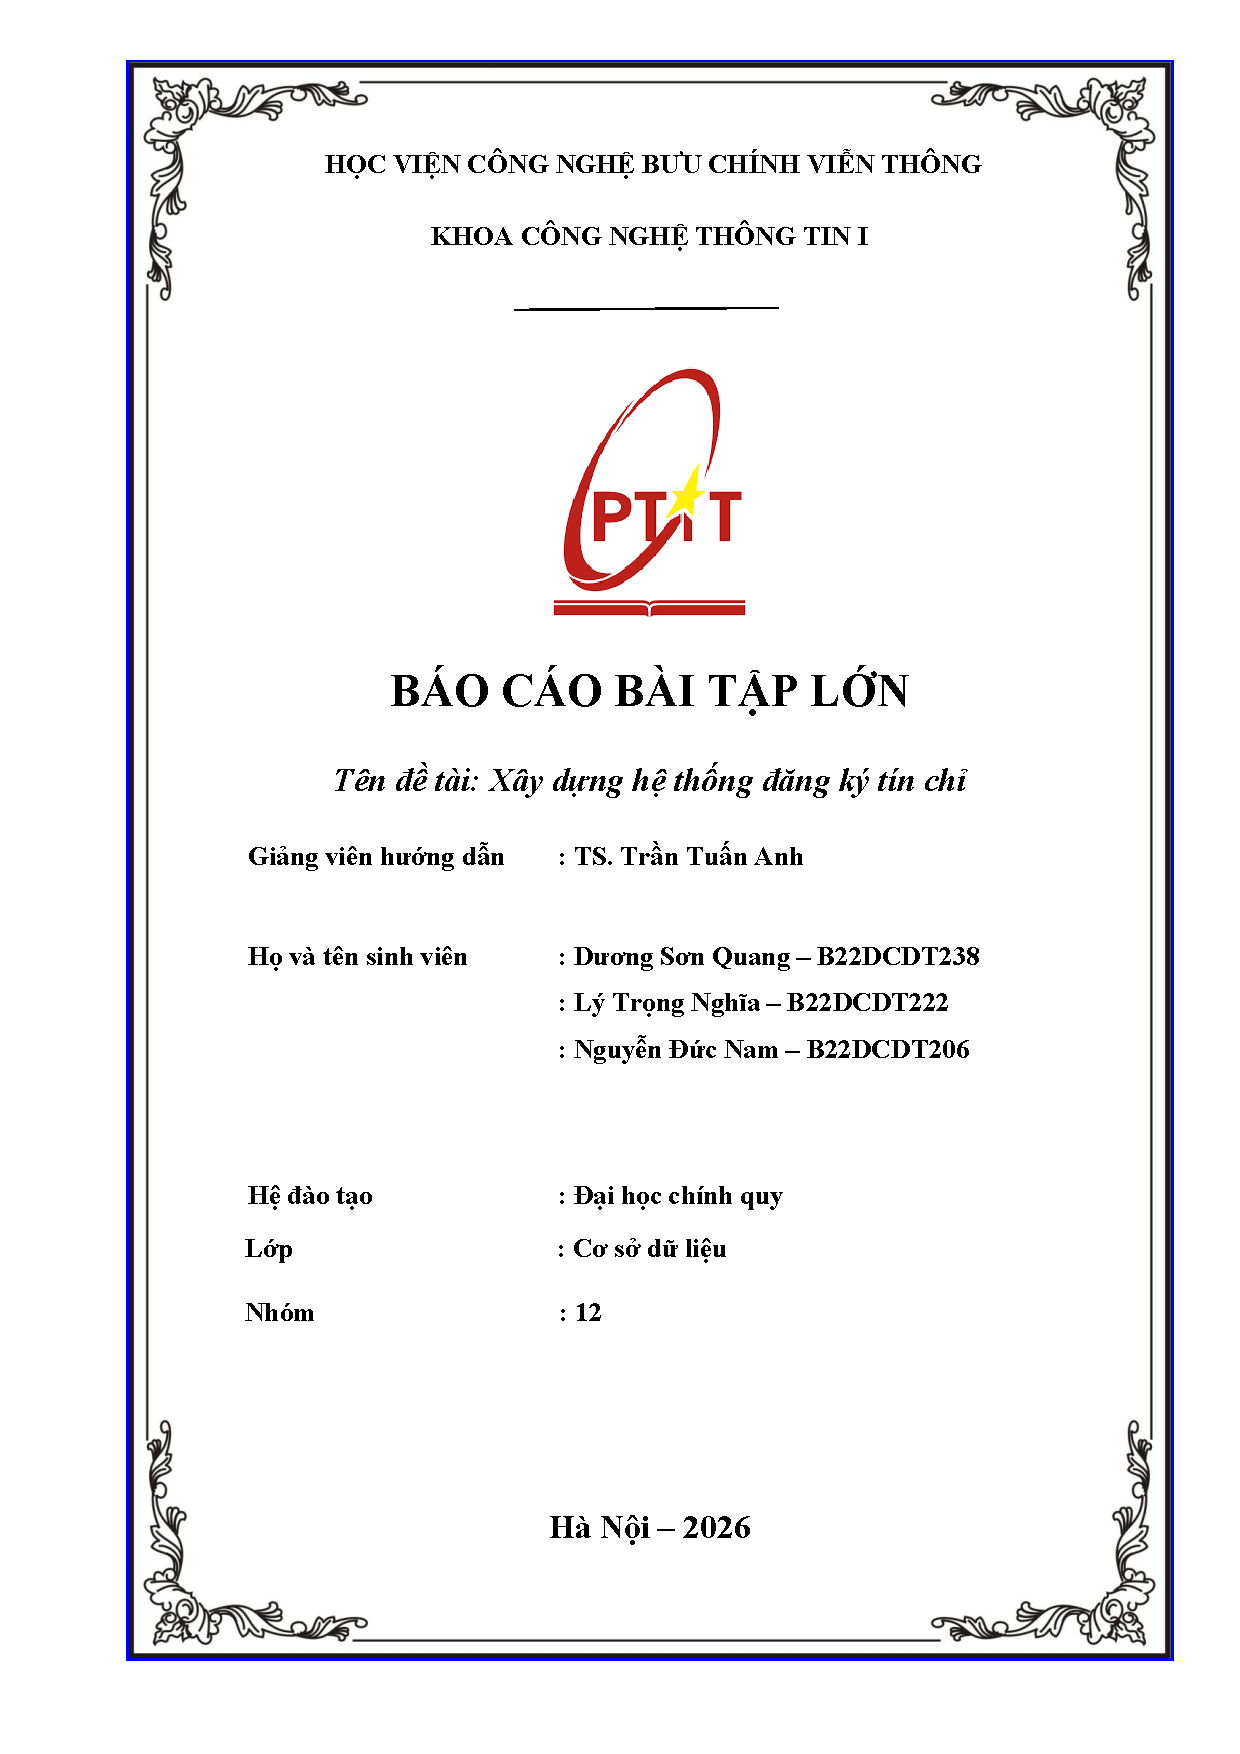
\includepdf[pages=1,pagecommand={\thispagestyle{empty}}]{image/bia_csdl.pdf}

\pagenumbering{roman}

% ============================================================
%  LỜI NÓI ĐẦU
% ============================================================
\newpage
\section*{LỜI NÓI ĐẦU}
\addcontentsline{toc}{section}{Lời nói đầu}

\noindent Trong bối cảnh giáo dục đại học ngày càng phát triển và mở rộng quy mô, việc quản lý đăng ký tín chỉ cho sinh viên trở thành một bài toán quan trọng và phức tạp. Hệ thống đăng ký tín chỉ không chỉ đơn thuần lưu trữ thông tin học tập mà còn phải đảm bảo tính toàn vẹn dữ liệu, kiểm tra các ràng buộc nghiệp vụ như tiên quyết môn học, giới hạn tín chỉ mỗi học kỳ, sỹ số lớp học phần và không trùng lịch học.

\vspace{0.4cm}
\noindent Bài tập lớn này trình bày toàn bộ quá trình thiết kế và xây dựng hệ thống cơ sở dữ liệu quản lý đăng ký tín chỉ cho ngành \textbf{Kỹ thuật Điện--Điện tử, Học viện Công nghệ Bưu chính Viễn thông (PTIT) Hà Nội}. Hệ thống được thiết kế với 7 module chức năng bao gồm: chương trình đào tạo, lịch học chuẩn hóa, tách đăng ký và kết quả học tập, quản lý học phí tự động, kiểm tra trùng lịch, 5 view phân tích và phân quyền hệ thống.

\vspace{0.4cm}
\noindent Nội dung báo cáo bao gồm: Phần~I trình bày các quy tắc nghiệp vụ và mô hình ER; Phần~II mô tả quá trình chuyển đổi sang mô hình quan hệ; Phần~III xác định đầy đủ các loại khoá; Phần~IV thực hiện chuẩn hoá lược đồ; Phần~V trình bày các câu lệnh SQL từ cơ bản đến nâng cao bao gồm DDL, DML, Stored Procedure, Trigger, View, Chỉ mục và Phân quyền.

\vspace{0.4cm}
\noindent Nhóm chúng em xin chân thành cảm ơn thầy/cô đã hướng dẫn và cung cấp kiến thức nền tảng trong suốt quá trình học tập. Mặc dù đã cố gắng hết sức, báo cáo vẫn không tránh khỏi những thiếu sót, rất mong nhận được sự góp ý của thầy/cô.

\vspace{1cm}
\begin{flushright}
  \itshape Hà Nội, tháng 3 năm 2025 \\
  \bfseries Nhóm sinh viên thực hiện
\end{flushright}

% ============================================================
%  MỤC LỤC
% ============================================================
\newpage
\renewcommand{\contentsname}{MỤC LỤC}
\tableofcontents

\newpage
\pagenumbering{arabic}

% ============================================================
%  PHẦN I
% ============================================================
\section{PHẦN I: XÁC ĐỊNH CÁC QUY TẮC / RÀNG BUỘC VÀ XÂY DỰNG MÔ HÌNH THỰC THỂ LIÊN KẾT ER}

\subsection{Tổng quan hệ thống}

\noindent Hệ thống Quản lý đào tạo được xây dựng nhằm phục vụ công tác quản lý thông tin học tập tại ngành Kỹ thuật Điện--Điện tử, Học viện Công nghệ Bưu chính Viễn thông, với đầy đủ các chức năng từ quản lý chương trình đào tạo, lịch học, đăng ký tín chỉ đến theo dõi kết quả và học phí.

\begin{center}
\begin{tabular}{ll}
  \textbf{Tên hệ thống:} & Quản lý đào tạo  \\
  \textbf{Phạm vi:}      & Ngành KT Điện-Điện tử, PTIT Hà Nội \\
  \textbf{Hệ quản trị:}  & SQL Server (T-SQL)
\end{tabular}
\end{center}

\begin{table}[H]
\centering
\renewcommand{\arraystretch}{1.35}
\begin{tabular}{>{\centering}p{0.5cm} p{4cm} p{8.5cm}}
  \rowcolor{tableheadbg}
  \textcolor{white}{\textbf{\#}} &
  \textcolor{white}{\textbf{Module}} &
  \textcolor{white}{\textbf{Mô tả}} \\
  \rowcolor{white}      1 & Chương trình đào tạo & Quản lý lộ trình môn học theo từng khóa \\
  \rowcolor{tablerowalt}2 & Lịch học chuẩn hóa   & Lưu lịch học thành bảng riêng, hỗ trợ nhiều buổi/lớp \\
  \rowcolor{white}      3 & Tách đăng ký/kết quả & DANGKY (hành động) tách khỏi KETQUA\_HOCTAP (điểm) \\
  \rowcolor{tablerowalt}4 & Học phí tự động       & Tính học phí real-time qua trigger \\
  \rowcolor{white}      5 & Kiểm tra trùng lịch   & Trigger ngăn đăng ký 2 lớp cùng giờ \\
  \rowcolor{tablerowalt}6 & 5 View phân tích      & V\_BangDiem, V\_TinChiTichLuy, V\_GPA, V\_SinhVienNoMon, V\_MonDongNhat \\
  \rowcolor{white}      7 & Phân quyền hệ thống   & 3 ROLE: SinhVienRole, GiangVienRole, QuanTriRole \\
\end{tabular}
\caption{7 module chức năng của hệ thống}
\end{table}

\subsection{Các quy tắc và ràng buộc nghiệp vụ}

\subsubsection{Quy tắc về sinh viên}
\begin{itemize}[leftmargin=1.5cm]
  \item Mỗi sinh viên phải có mã sinh viên (\texttt{MaSV}) duy nhất trong toàn trường.
  \item Mỗi sinh viên thuộc về đúng một lớp hành chính (\texttt{LOPHOC}).
  \item Mỗi sinh viên chỉ được đăng ký \textbf{một lần} cho một lớp học phần trong bất kỳ đợt đăng ký nào.
  \item Mỗi học kỳ, sinh viên phải đăng ký \textbf{tối thiểu 10 tín chỉ} và \textbf{tối đa 25 tín chỉ}.
  \item Kết quả học tập của sinh viên được lưu theo \textbf{từng lần học} (\texttt{LanHoc}), hỗ trợ học lại nhiều lần.
\end{itemize}

\subsubsection{Quy tắc về môn học và tiên quyết}
\begin{itemize}[leftmargin=1.5cm]
  \item Mỗi môn học có số tín chỉ từ 1 đến 6, phân loại là \emph{Bắt buộc} hoặc \emph{Tự chọn}.
  \item Một môn học có thể có nhiều môn tiên quyết. Sinh viên phải \textbf{đạt} (có lần học với \texttt{TrangThai = 'Dat'} và điểm $\geq$ \texttt{DiemMin}) môn tiên quyết trước khi đăng ký.
  \item Một môn học \textbf{không thể} là tiên quyết của chính nó.
  \item Mỗi ngành/khóa có một \textbf{chương trình đào tạo} riêng, định nghĩa lộ trình môn học và học kỳ đề xuất.
\end{itemize}

\subsubsection{Quy tắc về lớp học phần và lịch học}
\begin{itemize}[leftmargin=1.5cm]
  \item Mỗi lớp học phần được mở cho một môn học cụ thể, do một giáo viên phụ trách.
  \item Sỹ số tối đa nằm trong khoảng từ 10 đến 100 sinh viên.
  \item Một giáo viên không được dạy hai lớp học phần của cùng một môn trong cùng học kỳ và năm học.
  \item Số sinh viên đã đăng ký \textbf{không được vượt quá} sỹ số tối đa (kiểm tra ở cả Stored Procedure và Trigger).
  \item Mỗi lớp học phần có thể có \textbf{nhiều buổi học} (lý thuyết + thực hành) được lưu trong bảng LICHHOC với thứ trong tuần (\texttt{Thu}: 2--7) và tiết bắt đầu (\texttt{TietBatDau}: 1--14).
  \item Sinh viên \textbf{không được đăng ký} hai lớp học phần có lịch học trùng nhau trong cùng đợt.
\end{itemize}

\subsubsection{Quy tắc về đợt đăng ký}
\begin{itemize}[leftmargin=1.5cm]
  \item Mỗi học kỳ, năm học chỉ có \textbf{duy nhất một} đợt đăng ký (ràng buộc \texttt{UNIQUE(HocKy, NamHoc)}).
  \item Ngày kết thúc đợt đăng ký phải sau ngày bắt đầu.
  \item Trạng thái đợt đăng ký chỉ nhận: \emph{Sắp tới}, \emph{Đang mở}, \emph{Đã đóng}.
  \item Sinh viên chỉ được đăng ký khi đợt đăng ký đang ở trạng thái ``\emph{Đang mở}''.
  \item Sinh viên chỉ được hủy đăng ký khi đợt đăng ký vẫn còn ``\emph{Đang mở}''.
\end{itemize}

\subsubsection{Quy tắc về bảo mật đăng nhập}
\begin{itemize}[leftmargin=1.5cm]
  \item Cả hai thực thể \textbf{GIAOVIEN} và \textbf{SINHVIEN} đều có thuộc tính \texttt{MatKhau} để xác thực đăng nhập vào hệ thống.
  \item Mật khẩu \textbf{không được lưu dưới dạng văn bản thuần} (plain text); hệ thống lưu \textbf{giá trị băm} (hash) theo chuẩn SHA-256, kiểu \texttt{NVARCHAR(256)}.
  \item Mật khẩu là thuộc tính \textbf{NOT NULL} -- mọi tài khoản phải được cấp mật khẩu ngay khi khởi tạo.
  \item Việc xác thực đăng nhập được thực hiện ở tầng ứng dụng: ứng dụng băm mật khẩu người dùng nhập vào rồi so sánh với giá trị đã lưu -- \textbf{không truy vấn mật khẩu} trực tiếp qua SQL.
  \item Mật khẩu mặc định khi khởi tạo tài khoản giáo viên là hash của \texttt{MaGV}, sinh viên là hash của \texttt{MaSV} (dễ bàn giao, bắt buộc đổi lần đầu đăng nhập).
\end{itemize}

\subsubsection{Quy tắc về học phí}
\begin{itemize}[leftmargin=1.5cm]
  \item Học phí được tính tự động mỗi khi sinh viên đăng ký hoặc hủy đăng ký môn học (qua Trigger \texttt{TRG\_TinhHocPhi}).
  \item Đơn giá chuẩn là \textbf{700.000 VND/tín chỉ} (theo mức học phí PTIT năm 2024).
  \item Tổng tiền học phí (\texttt{TongTien}) là cột tính toán tự động: $\texttt{TongTien} = \texttt{SoTinChi} \times \texttt{DonGia}$ (PERSISTED).
\end{itemize}

\subsection{Danh sách các thực thể (Entity)}

\noindent Hệ thống gồm \textbf{14 bảng} bao gồm các thực thể mạnh, thực thể yếu, thực thể liên kết và 1 mối quan hệ đệ quy M:N:

\begin{table}[H]
\centering
\renewcommand{\arraystretch}{1.35}
\begin{tabular}{>{\centering}p{0.8cm} >{\bfseries}p{3.6cm} p{2.2cm} p{3cm} p{4cm}}
  \rowcolor{tableheadbg}
  \textcolor{white}{\textbf{STT}} &
  \textcolor{white}{Tên Bảng} &
  \textcolor{white}{\textbf{Loại}} &
  \textcolor{white}{\textbf{Khoá Chính}} &
  \textcolor{white}{\textbf{Mô Tả}} \\
  \rowcolor{white}
  1 & GIAOVIEN             & Mạnh     & MaGV            & Thông tin giáo viên, có \texttt{MatKhau} đăng nhập \\
  \rowcolor{tablerowalt}
  2 & MONHOC               & Mạnh     & MaMon           & Thông tin môn học \\
  \rowcolor{white}
  3 & CHUONGTRINH\_DAOTAO  & Mạnh     & MaCT            & Chương trình đào tạo \\
  \rowcolor{tablerowalt}
  4 & LOPHOC               & Mạnh     & MaLop           & Lớp hành chính \\
  \rowcolor{white}
  5 & SINHVIEN             & Mạnh     & MaSV            & Thông tin sinh viên, có \texttt{MatKhau} đăng nhập \\
  \rowcolor{tablerowalt}
  6 & QUANTRI              & Mạnh     & MaQT            & Tài khoản quản trị hệ thống \\
  \rowcolor{white}
  7 & DOTDANGKY            & Mạnh     & MaDot           & Đợt đăng ký tín chỉ \\
  \rowcolor{tablerowalt}
  8 & LOPHOCPHAN           & Mạnh     & MaLopHP         & Lớp học phần \\
  \rowcolor{white}
  9 & LICHHOC              & Yếu      & MaLich (IDENTITY) & Lịch học của lớp học phần \\
  \rowcolor{tablerowalt}
  10 & DANGKY              & Liên kết & (MaSV, MaLopHP) & Hành động đăng ký học phần \\
  \rowcolor{white}
  11 & KETQUA\_HOCTAP      & Mạnh     & (MaSV, MaMon, LanHoc) & Điểm và lịch sử học lại \\
  \rowcolor{tablerowalt}
  12 & HOCPHI              & Mạnh     & (MaSV, HocKy, NamHoc) & Học phí theo học kỳ \\
  \rowcolor{white}
  13 & CTDT\_MONHOC        & Liên kết & (MaCT, MaMon)   & Môn học trong chương trình đào tạo \\
  \rowcolor{tablerowalt}
  14 & YEUCAU\_TIENQUYET   & Liên kết & (MonChinh, MonTienQuyet) & Quan hệ đệ quy M:N -- điều kiện tiên quyết \\
\end{tabular}
\caption{Danh sách 14 bảng trong hệ thống}
\end{table}

\subsection{Thuộc tính của các thực thể}

\subsubsection{Thực thể GIAOVIEN}
\begin{sqlbox}[Thuộc tính GIAOVIEN]
GIAOVIEN {
   MaGV (PK)    : VARCHAR(10)    -- Ma giao vien
   TenGV        : NVARCHAR(50)   -- Ho va ten
   ChuyenNganh  : NVARCHAR(50)   -- Chuyen nganh giang day
   HocVi        : NVARCHAR(30)   -- Cu nhan/Thac si/Tien si/GS/PGS
   Khoa         : NVARCHAR(50)   -- Khoa phu trach
   Email        : VARCHAR(50)    -- Email (duy nhat)
   DienThoai    : VARCHAR(10)    -- So dien thoai
   MatKhau      : NVARCHAR(256)  -- Hash SHA-256 mat khau dang nhap
                                 -- Mac dinh: hash(MaGV), bat buoc doi lan dau
                                 -- KHONG luu plain text
}
\end{sqlbox}

\subsubsection{Thực thể SINHVIEN}
\begin{sqlbox}[Thuộc tính SINHVIEN]
SINHVIEN {
   MaSV (PK)    : VARCHAR(10)    -- Ma sinh vien
   TenSV        : NVARCHAR(50)   -- Ho va ten
   NamNhapHoc   : INT            -- Nam bat dau hoc
   ChuyenNganh  : NVARCHAR(50)   -- Chuyen nganh hoc
   MaLop (FK)   : VARCHAR(10)    -- -> LOPHOC
   Email        : VARCHAR(50)    -- Email (duy nhat)
   DienThoai    : VARCHAR(10)    -- So dien thoai
   MatKhau      : NVARCHAR(256)  -- Hash SHA-256 mat khau dang nhap
                                 -- Mac dinh: hash(MaSV), bat buoc doi lan dau
                                 -- KHONG luu plain text
}
\end{sqlbox}

\subsubsection{Thực thể CHUONGTRINH\_DAOTAO và bảng liên kết CTDT\_MONHOC}
\begin{sqlbox}[Thuộc tính CHUONGTRINH\_DAOTAO và CTDT\_MONHOC]
CHUONGTRINH_DAOTAO {
   MaCT (PK)      : VARCHAR(10)    -- Ma chuong trinh dao tao
   TenCT          : NVARCHAR(100)  -- Ten chuong trinh
   Nganh          : NVARCHAR(100)  -- Ten nganh hoc
   NamApDung      : INT            -- Nam bat dau ap dung
}

-- Bang lien ket M:N giua CHUONGTRINH_DAOTAO va MONHOC
-- PK = (MaCT, MaMon)
CTDT_MONHOC {
   MaCT (PK, FK)    : VARCHAR(10)  -- -> CHUONGTRINH_DAOTAO
   MaMon (PK, FK)   : VARCHAR(10)  -- -> MONHOC
   HocKyDeXuat      : INT          -- Hoc ky de xuat hoc mon nay (1-10)
   BatBuoc          : BIT          -- 1=Bat buoc, 0=Tu chon trong CT
}
\end{sqlbox}

\subsubsection{Thực thể LOPHOCPHAN}
\begin{sqlbox}[Thuộc tính LOPHOCPHAN]
LOPHOCPHAN {
   MaLopHP (PK) : VARCHAR(15)   -- Ma lop hoc phan
   MaMon (FK)   : VARCHAR(10)   -- -> MONHOC
   MaGV (FK)    : VARCHAR(10)   -- -> GIAOVIEN
   MaDot (FK)   : VARCHAR(10)   -- -> DOTDANGKY
   SysoMax      : INT           -- Sy so toi da (10-100)
   -- Phong va lich hoc duoc luu trong bang LICHHOC
   -- Mot lop co the co nhieu buoi hoc (ly thuyet + thuc hanh)
}
\end{sqlbox}

\subsubsection{Thực thể yếu LICHHOC}
\begin{sqlbox}[Thuộc tính LICHHOC -- thực thể yếu phụ thuộc LOPHOCPHAN]
LICHHOC {
   MaLich (PK)  : INT IDENTITY   -- Surrogate key tu tang
   MaLopHP (FK) : VARCHAR(15)    -- -> LOPHOCPHAN (ON DELETE CASCADE)
   Thu          : INT             -- Thu trong tuan: 2=Thu Hai...7=Thu Bay
   TietBatDau   : INT             -- Tiet bat dau (1-14)
   SoTiet       : INT             -- So tiet moi buoi (1-6)
   Phong        : NVARCHAR(20)    -- Phong hoc
   -- Kiem tra trung lich: [A, A+sA) giao [B, B+sB) != null
   -- <=> A < B+sB AND B < A+sA
}
\end{sqlbox}

\subsubsection{Bảng DANGKY}
\begin{sqlbox}[Thuộc tính DANGKY -- lưu hành động đăng ký, không lưu điểm]
DANGKY {
   MaSV (PK, FK)    : VARCHAR(10)   -- -> SINHVIEN
   MaLopHP (PK, FK) : VARCHAR(15)   -- -> LOPHOCPHAN
   NgayDangKy       : DATE          -- Ngay thuc hien dang ky
   TrangThai        : NVARCHAR(20)  -- 'Cho xac nhan'/'Da xac nhan'/'Da huy'
   -- KHONG co cot Diem: diem so duoc luu rieng trong KETQUA_HOCTAP
   -- KHONG luu MaDot: tranh phu thuoc bac cau -> lay qua LOPHOCPHAN.MaDot
}
\end{sqlbox}

\subsubsection{Thực thể KETQUA\_HOCTAP}
\begin{sqlbox}[Thuộc tính KETQUA\_HOCTAP -- lưu điểm và lịch sử học lại]
KETQUA_HOCTAP {
   MaSV (PK, FK)  : VARCHAR(10)   -- -> SINHVIEN
   MaMon (PK, FK) : VARCHAR(10)   -- -> MONHOC (khong phai MaLopHP)
   LanHoc (PK)    : INT           -- Lan hoc thu may (1, 2, 3...)
   HocKy          : INT           -- Hoc ky hoc mon nay
   NamHoc         : INT           -- Nam hoc
   Diem           : DECIMAL(4,2)  -- Diem (0-10), NULL neu chua co
   TrangThai      : NVARCHAR(20)  -- 'Dat'/'Khong dat'/'Chua co diem'
   -- PK (MaSV, MaMon, LanHoc): ho tro hoc lai nhieu lan
   -- Tach roi khoi DANGKY: ket qua ton tai doc lap sau khi hoc xong
}
\end{sqlbox}

\subsubsection{Thực thể HOCPHI}
\begin{sqlbox}[Thuộc tính HOCPHI -- học phí được tính tự động qua trigger]
HOCPHI {
   MaSV (PK, FK)  : VARCHAR(10)   -- -> SINHVIEN
   HocKy (PK)     : INT           -- Hoc ky (1/2/3)
   NamHoc (PK)    : INT           -- Nam hoc
   SoTinChi       : INT           -- Tong TC dang ky HK nay
   DonGia         : MONEY         -- Don gia/TC (mac dinh 700,000 VND)
   TongTien       : AS (SoTinChi * DonGia) PERSISTED  -- Cot tinh toan
   TrangThai      : NVARCHAR(20)  -- 'Chua thanh toan'/'Da thanh toan'/'Mien giam'
   -- Duoc cap nhat tu dong boi TRG_TinhHocPhi khi INSERT/DELETE DANGKY
}
\end{sqlbox}

\subsection{Các mối quan hệ giữa thực thể}

\begin{table}[H]
\centering
\renewcommand{\arraystretch}{1.35}
\begin{tabular}{p{4.8cm} >{\centering}p{1.8cm} p{7cm}}
  \rowcolor{tableheadbg}
  \textcolor{white}{\textbf{Quan Hệ}} &
  \textcolor{white}{\textbf{Kiểu}} &
  \textcolor{white}{\textbf{Mô Tả}} \\
  \rowcolor{white}
  SINHVIEN -- LOPHOC & 1 : N & Một lớp hành chính có nhiều sinh viên \\
  \rowcolor{tablerowalt}
  GIAOVIEN -- LOPHOC & 1 : N & Một GV có thể chủ nhiệm nhiều lớp \\
  \rowcolor{white}
  MONHOC -- LOPHOCPHAN & 1 : N & Một môn có thể mở nhiều lớp học phần \\
  \rowcolor{tablerowalt}
  GIAOVIEN -- LOPHOCPHAN & 1 : N & Một GV có thể dạy nhiều lớp HP \\
  \rowcolor{white}
  DOTDANGKY -- LOPHOCPHAN & 1 : N & Một đợt DK chứa nhiều lớp HP \\
  \rowcolor{tablerowalt}
  LOPHOCPHAN -- LICHHOC & 1 : N & Một lớp HP có thể có nhiều buổi học \\
  \rowcolor{white}
  SINHVIEN -- DANGKY & 1 : N & Một SV có thể đăng ký nhiều lớp HP \\
  \rowcolor{tablerowalt}
  LOPHOCPHAN -- DANGKY & 1 : N & Một lớp HP có nhiều bản ghi đăng ký \\
  \rowcolor{white}
  SINHVIEN -- KETQUA\_HOCTAP & 1 : N & Một SV có nhiều kết quả học tập \\
  \rowcolor{tablerowalt}
  MONHOC -- KETQUA\_HOCTAP & 1 : N & Một môn có nhiều bản ghi kết quả \\
  \rowcolor{white}
  SINHVIEN -- HOCPHI & 1 : N & Một SV có học phí theo từng HK \\
  \rowcolor{tablerowalt}
  CHUONGTRINH\_DAOTAO -- MONHOC & M : N & Qua CTDT\_MONHOC, lưu HocKyDeXuat và BatBuoc \\
  \rowcolor{white}
  MONHOC -- MONHOC & M : N đệ quy & Qua YEUCAU\_TIENQUYET, lưu DiemMin \\
\end{tabular}
\caption{Bảng các mối quan hệ trong hệ thống}
\end{table}

\subsection{Sơ đồ Thực thể - Liên kết (ERD)}

\noindent Dưới đây là sơ đồ Thực thể - Liên kết (ER) tổng thể của hệ thống Quản lý đào tạo, bao gồm đầy đủ các thực thể mạnh, thực thể yếu, thuộc tính dẫn xuất và các mối quan hệ nghiệp vụ:

\begin{figure}[H]
  \centering
  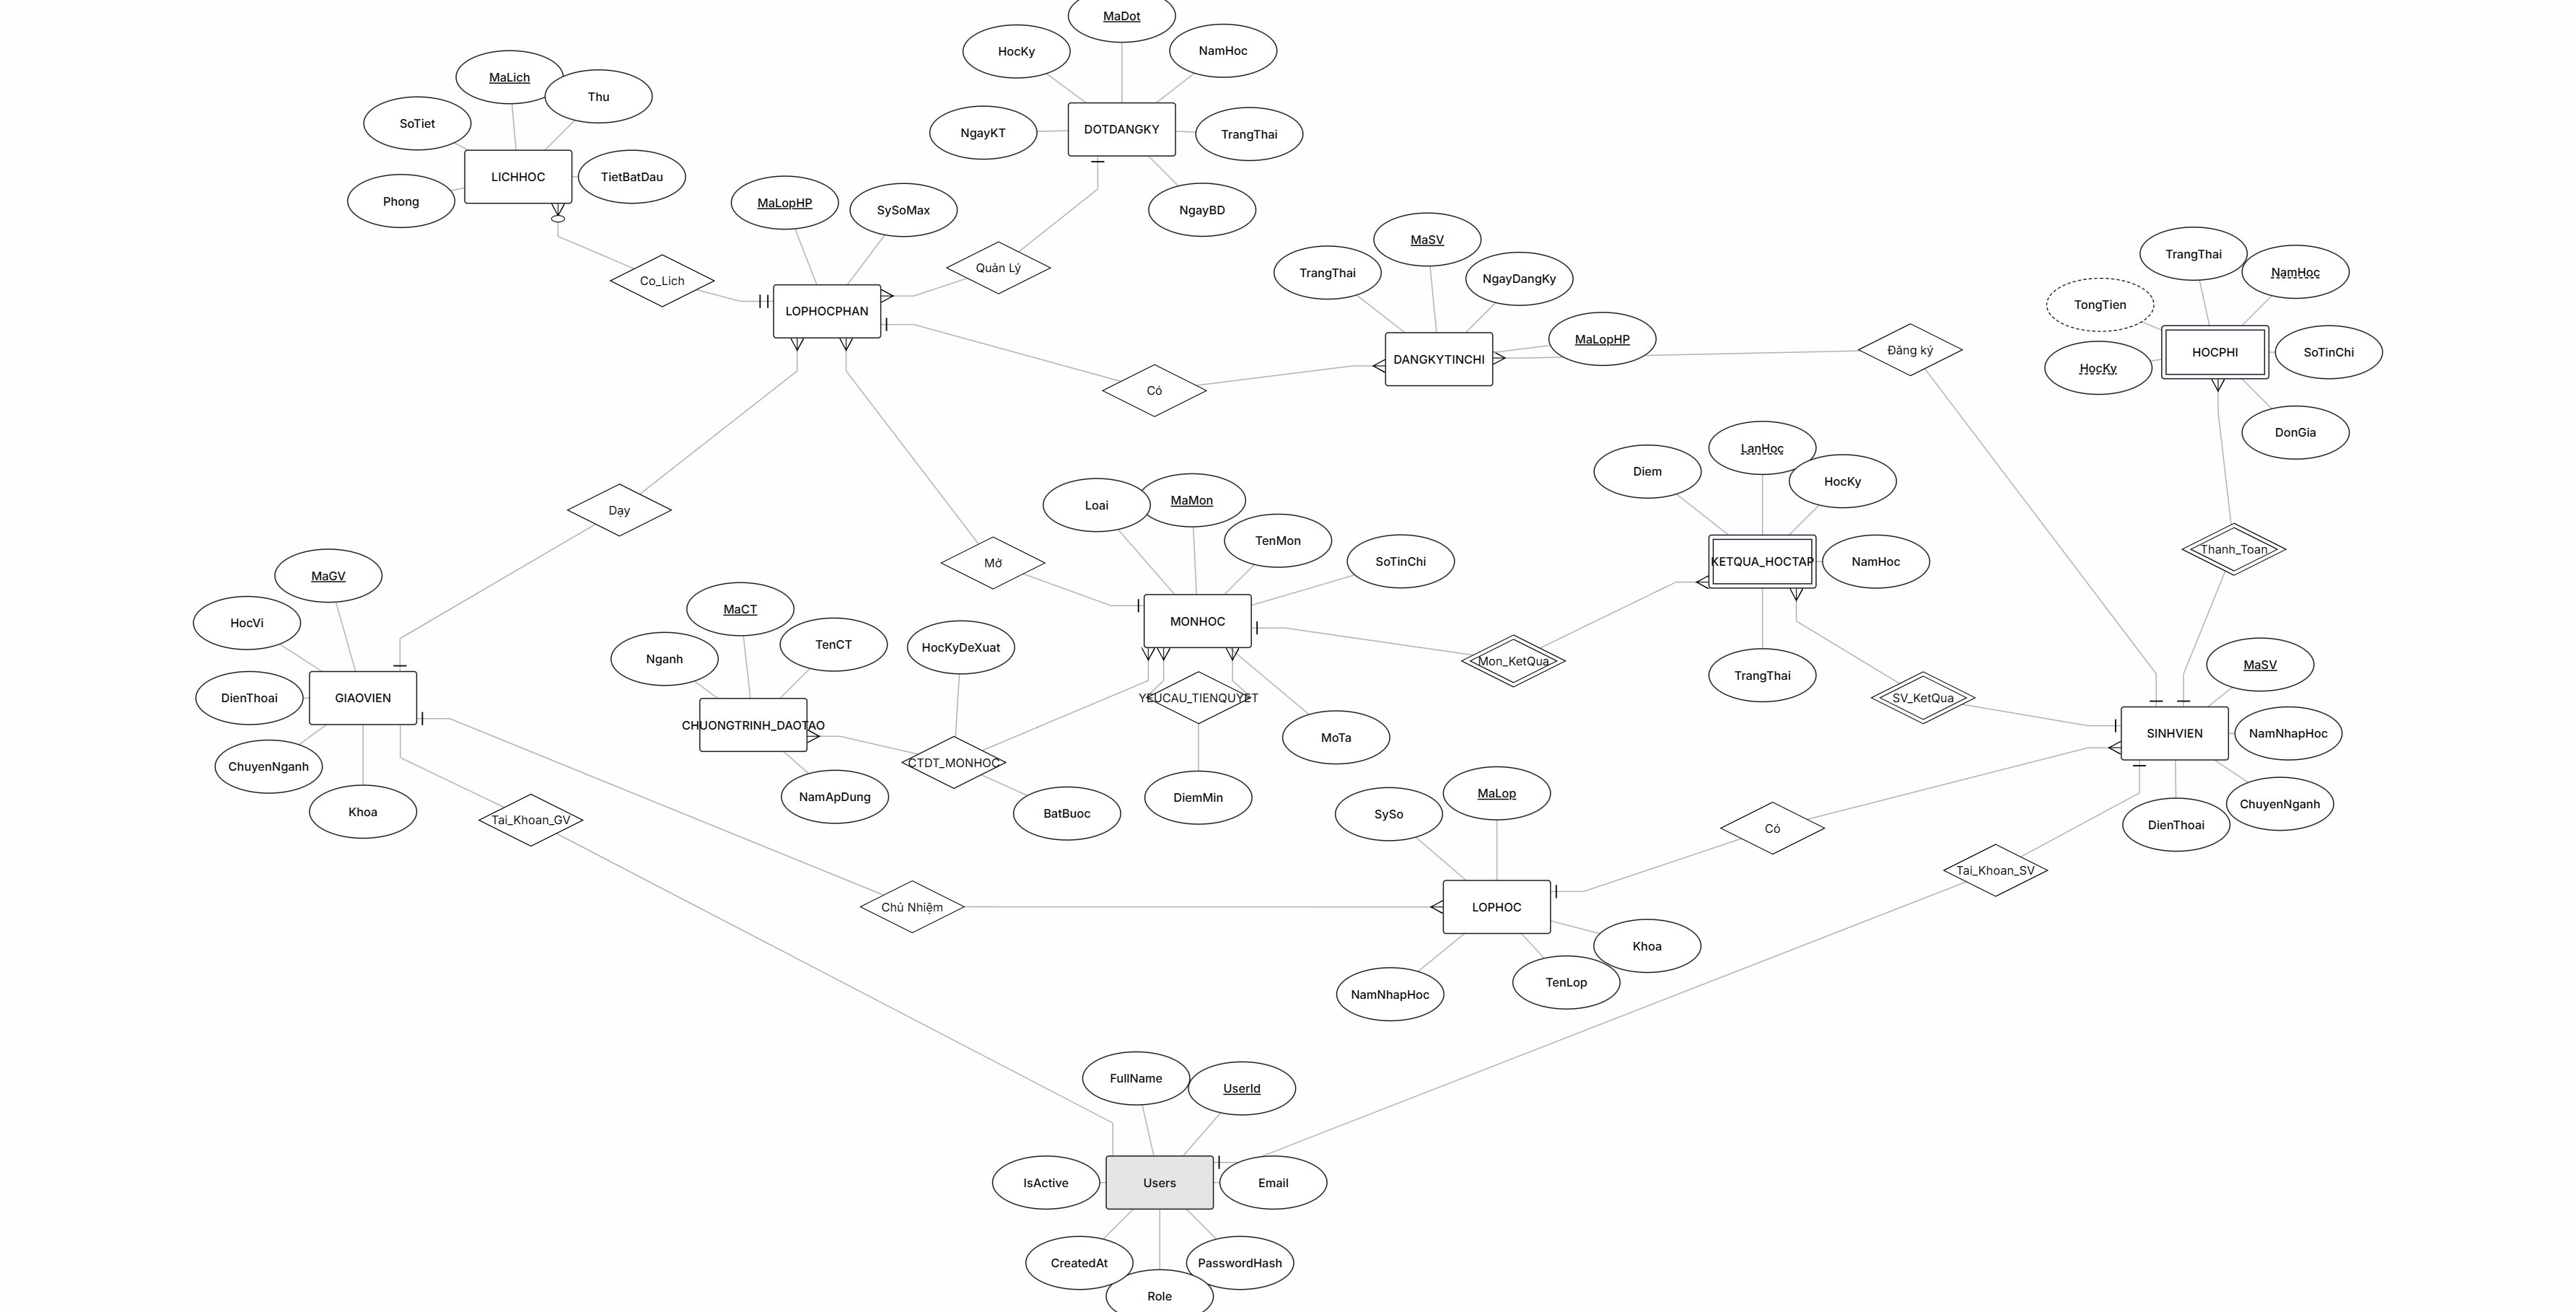
\includegraphics[width=\textwidth]{image/Mo_hinh_ER.png}
  \caption{Sơ đồ Thực thể - Liên kết (ER) hệ thống Quản lý đào tạo}
  \label{fig:er_diagram}
\end{figure}

% ============================================================
%  PHẦN II
% ============================================================
\newpage
\section{PHẦN II: CHUYỂN TỪ MÔ HÌNH ER SANG MÔ HÌNH QUAN HỆ}

\subsection{Lược đồ quan hệ mức logic}

\begin{sqlbox}[Lược đồ quan hệ mức logic -- toàn bộ 14 bảng]
-- ===== THỰC THỂ MẠNH =====
GIAOVIEN  (MaGV, TenGV, ChuyenNganh, HocVi, Khoa, Email, DienThoai, MatKhau)

MONHOC    (MaMon, TenMon, SoTinChi, Loai, MoTa)

CHUONGTRINH_DAOTAO (MaCT, TenCT, Nganh, NamApDung)

LOPHOC    (MaLop, TenLop, Khoa, MaGVChuNhiem -> GIAOVIEN, SySo, NamNhapHoc)

SINHVIEN  (MaSV, TenSV, NamNhapHoc, ChuyenNganh,
           MaLop -> LOPHOC, Email, DienThoai, MatKhau)

QUANTRI   (MaQT, TenQT, Email, MatKhau, DienThoai)

DOTDANGKY (MaDot, NamHoc, HocKy, NgayBD, NgayKT, TrangThai)

-- ===== LOPHOCPHAN =====
LOPHOCPHAN(MaLopHP, MaMon -> MONHOC, MaGV -> GIAOVIEN,
           MaDot -> DOTDANGKY, SysoMax)

-- ===== THỰC THỂ YẾU =====
LICHHOC   (MaLich IDENTITY, MaLopHP -> LOPHOCPHAN CASCADE,
           Thu, TietBatDau, SoTiet, Phong)

-- ===== BẢNG ĐỐI SÁNH ĐỢT ĐĂNG KÝ =====
DANGKY    (MaSV -> SINHVIEN, MaLopHP -> LOPHOCPHAN,
           NgayDangKy, TrangThai)
-- PK = (MaSV, MaLopHP); TrangThai: 'Cho xac nhan'/'Da xac nhan'/'Da huy'
-- KHONG co Diem (da tach sang KETQUA_HOCTAP)

KETQUA_HOCTAP (MaSV -> SINHVIEN, MaMon -> MONHOC, LanHoc,
               HocKy, NamHoc, Diem, TrangThai)
-- PK = (MaSV, MaMon, LanHoc): ho tro hoc lai nhieu lan
-- FK den MONHOC (khong phai LOPHOCPHAN): ton tai doc lap

HOCPHI    (MaSV -> SINHVIEN, HocKy, NamHoc,
           SoTinChi, DonGia, TongTien AS PERSISTED, TrangThai)
-- PK = (MaSV, HocKy, NamHoc); cap nhat tu dong boi trigger

-- ===== BẢNG LIÊN KẾT M:N =====
CTDT_MONHOC (MaCT -> CHUONGTRINH_DAOTAO, MaMon -> MONHOC,
             HocKyDeXuat, BatBuoc)
-- PK = (MaCT, MaMon)

YEUCAU_TIENQUYET (MonChinh -> MONHOC, MonTienQuyet -> MONHOC, DiemMin)
-- PK = (MonChinh, MonTienQuyet)
\end{sqlbox}

\vspace{0.5cm}
\noindent Để có cái nhìn trực quan hơn về cấu trúc vật lý, dưới đây là Sơ đồ Mô hình Quan hệ (Relational Schema) thể hiện rõ các khóa chính (PK), khóa ngoại (FK) và hướng tham chiếu giữa 14 bảng trong hệ thống:

\begin{figure}[H]
  \centering
  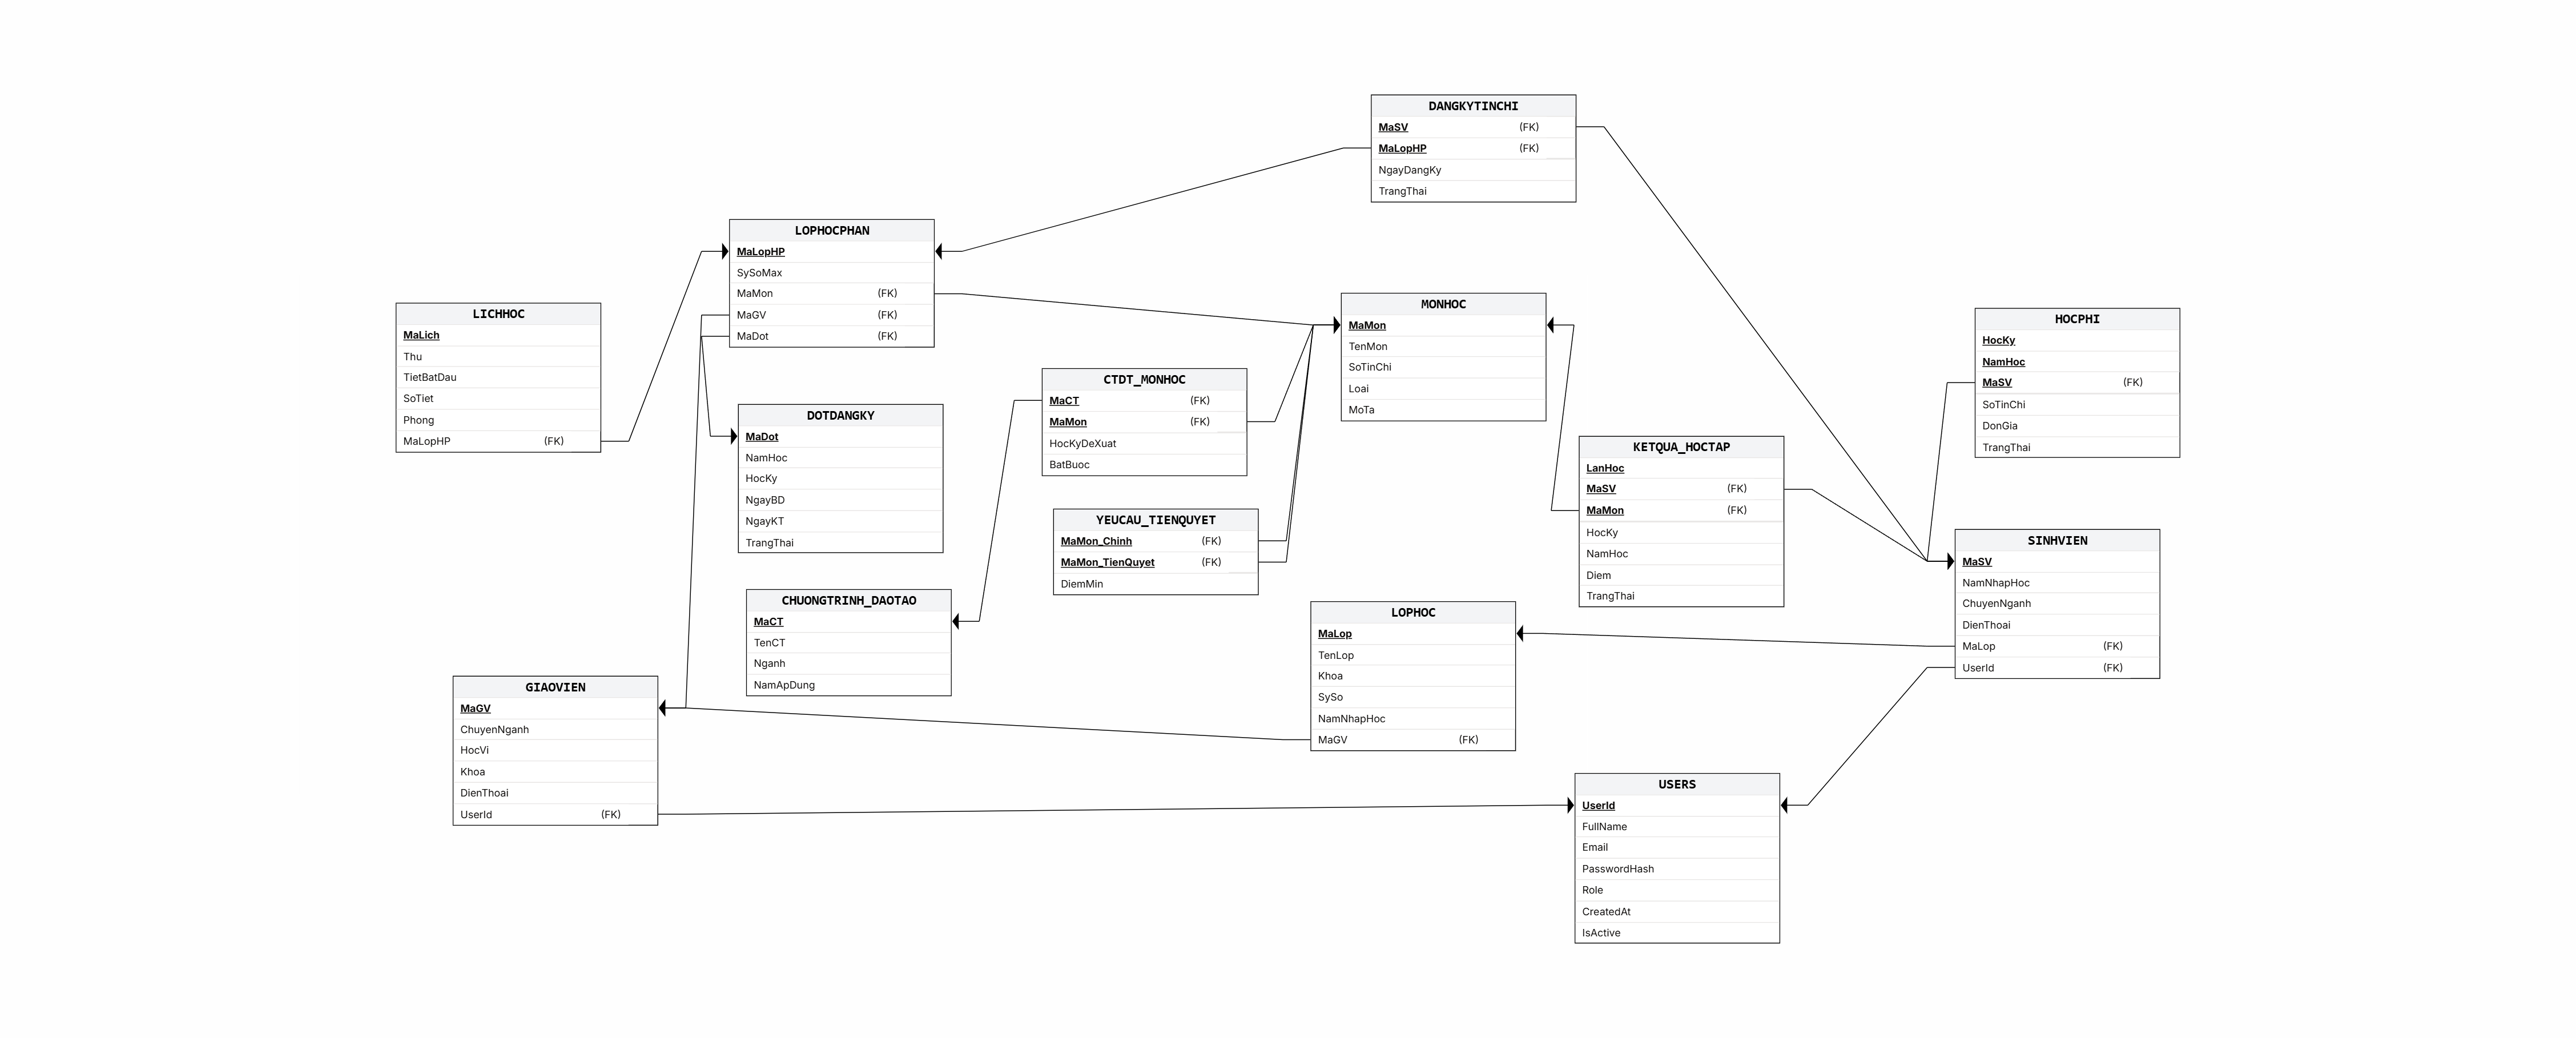
\includegraphics[width=\textwidth]{image/Luoc_do_quan_he.png}
  \caption{Sơ đồ Mô hình Quan hệ (Relational Schema) hệ thống}
  \label{fig:relational_schema}
\end{figure}

\subsection{Giải thích quá trình chuyển đổi}

\subsubsection{Tách DANGKY và KETQUA\_HOCTAP thành hai bảng độc lập}

\noindent Một quyết định thiết kế quan trọng là lưu thông tin đăng ký và điểm số vào hai bảng riêng biệt, thay vì gộp chung. Lý do:

\begin{itemize}[leftmargin=1.5cm]
  \item \textbf{Hỗ trợ học lại:} Kết quả học tập được xác định bởi PK tổ hợp \texttt{(MaSV, MaMon, LanHoc)}, cho phép lưu nhiều lần học một môn với điểm số khác nhau.
  \item \textbf{Tính độc lập của kết quả:} Điểm số là kết quả tồn tại lâu dài, không nên gắn chặt với một lớp học phần cụ thể -- sinh viên có thể có điểm dù bản ghi đăng ký không còn tồn tại.
  \item \textbf{Tránh dư thừa:} DANGKY chỉ lưu hành động đăng ký (ai đăng ký lớp nào, ngày nào, trạng thái xác nhận); KETQUA\_HOCTAP lưu kết quả học tập theo môn, độc lập với lớp học phần.
\end{itemize}

\subsubsection{Chuẩn hóa lịch học sang bảng LICHHOC}

\noindent Lịch học được lưu thành bảng riêng LICHHOC với các cột số \texttt{Thu}, \texttt{TietBatDau}, \texttt{SoTiet} thay vì chuỗi mô tả tự do. Thiết kế này mang lại hai lợi ích:

\begin{itemize}[leftmargin=1.5cm]
  \item Cho phép một lớp học phần có \textbf{nhiều buổi học} (lý thuyết + thực hành ở phòng khác nhau) -- mỗi buổi là một bản ghi độc lập trong LICHHOC.
  \item Cho phép kiểm tra trùng lịch chính xác bằng điều kiện số học: $A < B + s_B \text{ AND } B < A + s_A$, thay vì xử lý chuỗi phức tạp.
\end{itemize}

\subsubsection{Bảng CHUONGTRINH\_DAOTAO và CTDT\_MONHOC}

\noindent Quan hệ M:N giữa chương trình đào tạo và môn học được chuyển thành bảng liên kết CTDT\_MONHOC theo quy tắc chuyển đổi M:N. Bảng này lưu thêm thuộc tính \texttt{HocKyDeXuat} (học kỳ đề xuất học môn trong chương trình) và \texttt{BatBuoc} (1/0), phụ thuộc đầy đủ vào toàn bộ khoá tổ hợp \texttt{(MaCT, MaMon)}.

\subsubsection{Bảng HOCPHI và cột tính toán PERSISTED}

\noindent HOCPHI có khoá chính tổ hợp \texttt{(MaSV, HocKy, NamHoc)}. Cột \texttt{TongTien} là \emph{computed column} kiểu PERSISTED: giá trị được tính tự động từ \texttt{SoTinChi~*~DonGia} và được lưu vật lý trên đĩa (không tính lại mỗi lần đọc). Bảng này được cập nhật tự động bởi trigger \texttt{TRG\_TinhHocPhi} sau mỗi INSERT/DELETE trên DANGKY.

% ============================================================
%  PHẦN III
% ============================================================
\newpage
\section{PHẦN III: XÁC ĐỊNH KHOÁ}

\subsection{Khoá chính (Primary Key)}

\begin{table}[H]
\centering
\renewcommand{\arraystretch}{1.35}
\begin{tabular}{p{3.8cm} p{4cm} p{5.5cm}}
  \rowcolor{tableheadbg}
  \textcolor{white}{\textbf{Quan Hệ}} &
  \textcolor{white}{\textbf{Khoá Chính}} &
  \textcolor{white}{\textbf{Giải Thích}} \\
  \rowcolor{white}      GIAOVIEN              & MaGV                        & Mã GV cấp duy nhất toàn trường \\
  \rowcolor{tablerowalt}MONHOC                & MaMon                       & Mã môn học theo quy định nhà trường \\
  \rowcolor{white}      CHUONGTRINH\_DAOTAO   & MaCT                        & Mã chương trình đào tạo \\
  \rowcolor{tablerowalt}LOPHOC                & MaLop                       & Mã lớp hành chính \\
  \rowcolor{white}      SINHVIEN              & MaSV                        & Mã SV cấp khi nhập học \\
  \rowcolor{tablerowalt}QUANTRI               & MaQT                        & Mã quản trị viên \\
  \rowcolor{white}      DOTDANGKY             & MaDot                       & Mã đợt đăng ký \\
  \rowcolor{tablerowalt}LOPHOCPHAN            & MaLopHP                     & Mã lớp học phần \\
  \rowcolor{white}      LICHHOC               & MaLich (IDENTITY)           & Surrogate key tự tăng \\
  \rowcolor{tablerowalt}DANGKY                & (MaSV, MaLopHP)             & Composite PK từ quan hệ M:N \\
  \rowcolor{white}      KETQUA\_HOCTAP        & (MaSV, MaMon, LanHoc)       & Composite 3 thuộc tính, hỗ trợ học lại \\
  \rowcolor{tablerowalt}HOCPHI                & (MaSV, HocKy, NamHoc)       & Composite PK theo học kỳ \\
  \rowcolor{white}      CTDT\_MONHOC          & (MaCT, MaMon)               & Composite key tự nhiên M:N \\
  \rowcolor{tablerowalt}YEUCAU\_TIENQUYET     & (MonChinh, MonTienQuyet)    & Composite key tự nhiên M:N đệ quy \\
\end{tabular}
\caption{Khoá chính 14 bảng trong hệ thống}
\end{table}

\noindent \textbf{Lưu ý về LICHHOC:} Bảng này dùng surrogate key \texttt{MaLich IDENTITY} vì không có tập thuộc tính tự nhiên nào xác định duy nhất một buổi học -- cùng một lớp HP có thể có nhiều buổi học khác nhau, và cặp \texttt{(MaLopHP, Thu, TietBatDau)} lý thuyết là candidate key nhưng cấu trúc phức tạp hơn surrogate key.

\subsection{Khoá dự tuyển (Candidate Key)}

\begin{table}[H]
\centering
\renewcommand{\arraystretch}{1.35}
\begin{tabular}{p{3.5cm} p{5cm} p{5cm}}
  \rowcolor{tableheadbg}
  \textcolor{white}{\textbf{Quan Hệ}} &
  \textcolor{white}{\textbf{Khoá Dự Tuyển Bổ Sung}} &
  \textcolor{white}{\textbf{Lý Do}} \\
  \rowcolor{white}      GIAOVIEN     & Email                               & Email GV là duy nhất \\
  \rowcolor{tablerowalt}SINHVIEN     & Email                               & Email SV là duy nhất \\
  \rowcolor{white}      QUANTRI      & Email                               & Email quản trị là duy nhất \\
  \rowcolor{tablerowalt}LOPHOCPHAN   & (MaMon, MaGV, MaDot)               & GV không dạy cùng môn 2 lần/đợt \\
  \rowcolor{white}      DOTDANGKY    & (HocKy, NamHoc)                     & Mỗi HK/năm chỉ có 1 đợt DK \\
  \rowcolor{tablerowalt}LICHHOC      & (MaLopHP, Thu, TietBatDau)          & Xác định duy nhất một buổi học trong lớp \\
\end{tabular}
\caption{Khoá dự tuyển bổ sung (các bảng có composite PK không có khoá dự tuyển bổ sung)}
\end{table}

\subsection{Khoá ngoại (Foreign Key)}

\begin{table}[H]
\centering
\renewcommand{\arraystretch}{1.35}
\begin{tabular}{p{3cm} p{3cm} p{3.5cm} p{3.5cm}}
  \rowcolor{tableheadbg}
  \textcolor{white}{\textbf{Bảng}} &
  \textcolor{white}{\textbf{Khoá Ngoại}} &
  \textcolor{white}{\textbf{Tham Chiếu}} &
  \textcolor{white}{\textbf{Hành Động}} \\
  \rowcolor{white}      LOPHOC              & MaGVChuNhiem  & GIAOVIEN(MaGV)           & ON DELETE SET NULL \\
  \rowcolor{tablerowalt}SINHVIEN            & MaLop         & LOPHOC(MaLop)            & ON DELETE SET NULL \\
  \rowcolor{white}      LOPHOCPHAN          & MaMon         & MONHOC(MaMon)            & (mặc định) \\
  \rowcolor{tablerowalt}LOPHOCPHAN          & MaGV          & GIAOVIEN(MaGV)           & (mặc định) \\
  \rowcolor{white}      LOPHOCPHAN          & MaDot         & DOTDANGKY(MaDot)         & RESTRICT xóa \\
  \rowcolor{tablerowalt}LICHHOC             & MaLopHP       & LOPHOCPHAN(MaLopHP)      & ON DELETE CASCADE \\
  \rowcolor{white}      DANGKY              & MaSV          & SINHVIEN(MaSV)           & (mặc định) \\
  \rowcolor{tablerowalt}DANGKY              & MaLopHP       & LOPHOCPHAN(MaLopHP)      & (mặc định) \\
  \rowcolor{white}      KETQUA\_HOCTAP      & MaSV          & SINHVIEN(MaSV)           & (mặc định) \\
  \rowcolor{tablerowalt}KETQUA\_HOCTAP      & MaMon         & MONHOC(MaMon)            & (mặc định) \\
  \rowcolor{white}      HOCPHI              & MaSV          & SINHVIEN(MaSV)           & (mặc định) \\
  \rowcolor{tablerowalt}CTDT\_MONHOC        & MaCT          & CHUONGTRINH\_DAOTAO(MaCT) & (mặc định) \\
  \rowcolor{white}      CTDT\_MONHOC        & MaMon         & MONHOC(MaMon)            & (mặc định) \\
  \rowcolor{tablerowalt}YEUCAU\_TIENQUYET   & MonChinh      & MONHOC(MaMon)            & NO ACTION \\
  \rowcolor{white}      YEUCAU\_TIENQUYET   & MonTienQuyet  & MONHOC(MaMon)            & NO ACTION \\
\end{tabular}
\caption{Khoá ngoại và hành động tham chiếu trong hệ thống}
\end{table}

\noindent \textbf{Lưu ý đặc biệt:}
\begin{itemize}[leftmargin=1.5cm]
  \item \textbf{LICHHOC -- ON DELETE CASCADE:} Khi xóa một lớp học phần, toàn bộ lịch học của lớp đó cũng tự động bị xóa. Đây là hành vi đúng vì lịch học không có nghĩa khi lớp HP không còn tồn tại.
  \item \textbf{YEUCAU\_TIENQUYET -- NO ACTION:} Giữ nguyên để tránh lỗi SQL Server 1785 (cycles or multiple cascade paths) khi cả hai FK cùng trỏ về bảng MONHOC.
  \item \textbf{KETQUA\_HOCTAP không FK đến DANGKY:} Kết quả học tập tồn tại độc lập sau khi học xong -- sinh viên có thể có điểm dù bản ghi đăng ký không còn.
\end{itemize}

% ============================================================
%  PHẦN IV
% ============================================================
\newpage
\section{PHẦN IV: CHUẨN HÓA LƯỢC ĐỒ QUAN HỆ THÀNH DẠNG CHUẨN 3NF}

\subsection{Dạng chuẩn 1 (1NF)}

\noindent \textbf{Điều kiện 1NF:} Tất cả các thuộc tính phải có giá trị đơn trị, không có nhóm lặp lại.

\noindent Tất cả 14 bảng đều thoả mãn 1NF vì:
\begin{itemize}[leftmargin=1.5cm]
  \item Mỗi thuộc tính lưu một giá trị đơn. Đặc biệt, bảng LICHHOC lưu lịch học thành từng bộ \texttt{(Thu, TietBatDau, SoTiet)} -- mỗi buổi học là một bản ghi riêng biệt.
  \item Quan hệ đệ quy M:N và M:N thông thường đều được chuyển thành bảng riêng (YEUCAU\_TIENQUYET, CTDT\_MONHOC, DANGKY) với từng bộ xác định duy nhất.
  \item Cột tính toán \texttt{TongTien} trong HOCPHI là thuộc tính đơn trị (PERSISTED), không vi phạm 1NF.
\end{itemize}

\subsection{Dạng chuẩn 2 (2NF)}

\noindent \textbf{Điều kiện 2NF:} Thoả 1NF và không có phụ thuộc hàm bộ phận.

\begin{itemize}[leftmargin=1.5cm]
  \item \textbf{DANGKY:} PK = \texttt{(MaSV, MaLopHP)}. Thuộc tính \texttt{NgayDangKy} và \texttt{TrangThai} phụ thuộc đầy đủ vào cả hai khoá -- không thể suy ra từ \texttt{MaSV} hay \texttt{MaLopHP} riêng lẻ. $\Rightarrow$ \textbf{Đạt 2NF.}
  \item \textbf{KETQUA\_HOCTAP:} PK = \texttt{(MaSV, MaMon, LanHoc)}. Kiểm tra:
    \begin{itemize}[leftmargin=1cm]
      \item \texttt{(MaSV, MaMon)} $\to$ \texttt{Diem}? \textbf{Không} -- cùng SV cùng môn nhưng lần học khác nhau cho điểm khác nhau.
      \item $\Rightarrow$ \texttt{HocKy, NamHoc, Diem, TrangThai} phụ thuộc đầy đủ vào toàn bộ khoá tổ hợp. \checkmark
    \end{itemize}
  \item \textbf{CTDT\_MONHOC:} PK = \texttt{(MaCT, MaMon)}. Thuộc tính \texttt{HocKyDeXuat} phụ thuộc đầy đủ -- cùng một môn có thể được đề xuất ở học kỳ khác nhau tùy chương trình. $\Rightarrow$ \textbf{Đạt 2NF.}
  \item \textbf{HOCPHI:} PK = \texttt{(MaSV, HocKy, NamHoc)}. Các thuộc tính phụ thuộc đầy đủ vào cả ba khoá. $\Rightarrow$ \textbf{Đạt 2NF.}
  \item Các bảng có khoá chính đơn (GIAOVIEN, MONHOC, CHUONGTRINH\_DAOTAO, LOPHOC, SINHVIEN, DOTDANGKY, LOPHOCPHAN, LICHHOC) tự động đạt 2NF. \checkmark
\end{itemize}

\subsection{Dạng chuẩn 3 (3NF)}

\noindent \textbf{Điều kiện 3NF:} Thoả 2NF và không có phụ thuộc hàm bắc cầu.

\subsubsection{Phân tích bảng GIAOVIEN và SINHVIEN}
\textbf{Phụ thuộc hàm:}
\begin{itemize}[leftmargin=1.5cm]
  \item $\texttt{MaGV} \to \{\texttt{TenGV, ChuyenNganh, HocVi, Khoa, Email, DienThoai, MatKhau}\}$
  \item $\texttt{MaSV} \to \{\texttt{TenSV, NamNhapHoc, ChuyenNganh, MaLop, Email, DienThoai, MatKhau}\}$
\end{itemize}

\noindent Thuộc tính \texttt{MatKhau} phụ thuộc trực tiếp vào khoá chính đơn. Không tồn tại phụ thuộc bắc cầu nào liên quan vì:
\begin{itemize}[leftmargin=1.5cm]
  \item \texttt{MatKhau} là giá trị hash độc lập, không xác định và không được xác định bởi bất kỳ thuộc tính không khoá nào khác.
  \item Việc lưu hash thay vì plain text không tạo ra dư thừa dữ liệu -- mỗi tài khoản có đúng một giá trị hash duy nhất.
\end{itemize}
$\Rightarrow$ \textbf{GIAOVIEN và SINHVIEN đạt 3NF.}

\subsubsection{Phân tích bảng DANGKY}
\textbf{Phụ thuộc hàm:} $\texttt{(MaSV, MaLopHP)} \to \{\texttt{NgayDangKy, TrangThai}\}$

\noindent Không tồn tại phụ thuộc bắc cầu. \texttt{MaDot} không được lưu trong bảng này -- nếu giữ sẽ có chuỗi $\texttt{(MaSV,MaLopHP)} \to \texttt{MaLopHP} \to \texttt{MaDot}$ vi phạm 3NF. $\Rightarrow$ \textbf{Đạt 3NF.}

\subsubsection{Phân tích bảng KETQUA\_HOCTAP}
\textbf{Phụ thuộc hàm:} $\texttt{(MaSV, MaMon, LanHoc)} \to \{\texttt{HocKy, NamHoc, Diem, TrangThai}\}$

\noindent Kiểm tra phụ thuộc bắc cầu: \texttt{HocKy} và \texttt{NamHoc} không xác định các thuộc tính còn lại -- cùng học kỳ có nhiều sinh viên với điểm khác nhau. $\Rightarrow$ \textbf{Đạt 3NF.}

\noindent \textbf{Lý do không FK đến DOTDANGKY:} Kết quả học tập cần tồn tại độc lập, không gắn với một đợt đăng ký cụ thể. Điểm của lần học lại có thể thuộc đợt sau.

\subsubsection{Phân tích bảng HOCPHI}
\textbf{Phụ thuộc hàm:} $\texttt{(MaSV, HocKy, NamHoc)} \to \{\texttt{SoTinChi, DonGia, TongTien, TrangThai}\}$

\noindent \texttt{TongTien = SoTinChi * DonGia} là phụ thuộc hàm giữa các thuộc tính không khoá. Tuy nhiên, đây là \textbf{computed column PERSISTED} -- SQL Server không cho phép INSERT/UPDATE trực tiếp vào cột này; giá trị luôn được tính theo công thức. Đây là dạng chuẩn hóa đặc biệt được chấp nhận trong thực tế. $\Rightarrow$ \textbf{Đạt 3NF.}

\subsubsection{Phân tích bảng LICHHOC}
\textbf{Phụ thuộc hàm:} $\texttt{MaLich} \to \{\texttt{MaLopHP, Thu, TietBatDau, SoTiet, Phong}\}$

\noindent Mọi thuộc tính phụ thuộc trực tiếp vào khoá chính đơn \texttt{MaLich}. Không tồn tại phụ thuộc bắc cầu. $\Rightarrow$ \textbf{Đạt 3NF.}

\subsubsection{Phân tích bảng CTDT\_MONHOC}
\textbf{Phụ thuộc hàm:} $\texttt{(MaCT, MaMon)} \to \{\texttt{HocKyDeXuat, BatBuoc}\}$

\noindent Chỉ hai thuộc tính không khoá, cả hai phụ thuộc đầy đủ vào toàn bộ khoá tổ hợp. $\Rightarrow$ \textbf{Đạt 3NF.}

\subsubsection{Tổng kết chuẩn hóa}

\begin{table}[H]
\centering
\renewcommand{\arraystretch}{1.35}
\begin{tabular}{p{4.2cm} >{\centering}p{1.3cm} >{\centering}p{1.3cm} >{\centering}p{1.3cm} p{3.5cm}}
  \rowcolor{tableheadbg}
  \textcolor{white}{\textbf{Quan Hệ}} &
  \textcolor{white}{\textbf{1NF}} &
  \textcolor{white}{\textbf{2NF}} &
  \textcolor{white}{\textbf{3NF}} &
  \textcolor{white}{\textbf{Kết Luận}} \\
  \rowcolor{white}      GIAOVIEN              & \checkmark & \checkmark & \checkmark & Đạt 3NF \\
  \rowcolor{tablerowalt}MONHOC                & \checkmark & \checkmark & \checkmark & Đạt 3NF \\
  \rowcolor{white}      CHUONGTRINH\_DAOTAO   & \checkmark & \checkmark & \checkmark & Đạt 3NF \\
  \rowcolor{tablerowalt}LOPHOC                & \checkmark & \checkmark & \checkmark & Đạt 3NF \\
  \rowcolor{white}      SINHVIEN              & \checkmark & \checkmark & \checkmark & Đạt 3NF \\
  \rowcolor{tablerowalt}QUANTRI               & \checkmark & \checkmark & \checkmark & Đạt 3NF \\
  \rowcolor{white}      DOTDANGKY             & \checkmark & \checkmark & \checkmark & Đạt 3NF \\
  \rowcolor{tablerowalt}LOPHOCPHAN            & \checkmark & \checkmark & \checkmark & Đạt 3NF \\
  \rowcolor{white}      LICHHOC               & \checkmark & \checkmark & \checkmark & Đạt 3NF \\
  \rowcolor{tablerowalt}DANGKY                & \checkmark & \checkmark & \checkmark & Đạt 3NF \\
  \rowcolor{white}      KETQUA\_HOCTAP        & \checkmark & \checkmark & \checkmark & Đạt 3NF \\
  \rowcolor{tablerowalt}HOCPHI                & \checkmark & \checkmark & \checkmark & Đạt 3NF \\
  \rowcolor{white}      CTDT\_MONHOC          & \checkmark & \checkmark & \checkmark & Đạt 3NF \\
  \rowcolor{tablerowalt}YEUCAU\_TIENQUYET     & \checkmark & \checkmark & \checkmark & Đạt 3NF \& BCNF \\
\end{tabular}
\caption{Tổng kết kiểm tra chuẩn hóa 14 bảng của hệ thống}
\end{table}

% ============================================================
%  PHẦN V
% ============================================================
\newpage
\section{PHẦN V: CÂU LỆNH TRUY VẤN DỮ LIỆU SQL}

\subsection{DDL -- Tạo cấu trúc cơ sở dữ liệu}

\subsubsection{Khởi tạo database}

\begin{sqlbox}[Tạo database và dọn dẹp (thứ tự DROP: Views -> SPs -> Triggers -> Tables)]
IF DB_ID('QuanLyDangKyTinChi') IS NULL
    CREATE DATABASE QuanLyDangKyTinChi COLLATE Vietnamese_CI_AS;
GO
USE QuanLyDangKyTinChi;
GO

-- Views
DROP VIEW IF EXISTS V_MonDongNhat; DROP VIEW IF EXISTS V_SinhVienNoMon;
DROP VIEW IF EXISTS V_GPA;         DROP VIEW IF EXISTS V_BangDiem;
DROP VIEW IF EXISTS V_TinChiTichLuy;
GO
-- Stored Procedures
DROP PROCEDURE IF EXISTS SP_MonCoTheDangKy;  DROP PROCEDURE IF EXISTS SP_HuyDangKy;
DROP PROCEDURE IF EXISTS SP_DangKyTinChi;    DROP PROCEDURE IF EXISTS SP_RestoreDatabase;
DROP PROCEDURE IF EXISTS SP_BackupDatabase;
GO
-- Triggers
DROP TRIGGER IF EXISTS TRG_TinhHocPhi;    DROP TRIGGER IF EXISTS TRG_KiemTraTrungLich;
DROP TRIGGER IF EXISTS TRG_CapNhatKetQua; DROP TRIGGER IF EXISTS TRG_KiemTraSySo;
GO
-- Tables (nguoc chieu phu thuoc FK)
DROP TABLE IF EXISTS HOCPHI;          DROP TABLE IF EXISTS KETQUA_HOCTAP;
DROP TABLE IF EXISTS DANGKY;          DROP TABLE IF EXISTS LICHHOC;
DROP TABLE IF EXISTS YEUCAU_TIENQUYET; DROP TABLE IF EXISTS LOPHOCPHAN;
DROP TABLE IF EXISTS CTDT_MONHOC;     DROP TABLE IF EXISTS DOTDANGKY;
DROP TABLE IF EXISTS QUANTRI;         DROP TABLE IF EXISTS SINHVIEN;
DROP TABLE IF EXISTS LOPHOC;          DROP TABLE IF EXISTS CHUONGTRINH_DAOTAO;
DROP TABLE IF EXISTS MONHOC;          DROP TABLE IF EXISTS GIAOVIEN;
GO
\end{sqlbox}

\subsubsection{Tạo bảng GIAOVIEN, MONHOC và CHUONGTRINH\_DAOTAO}

\begin{sqlbox}[Tạo GIAOVIEN, MONHOC, CHUONGTRINH\_DAOTAO và CTDT\_MONHOC]
CREATE TABLE GIAOVIEN (
    MaGV        VARCHAR(10)   NOT NULL,
    TenGV       NVARCHAR(50)  NOT NULL,
    ChuyenNganh NVARCHAR(50),
    HocVi       NVARCHAR(30)  CHECK (HocVi IN
                (N'Cu nhan',N'Thac si',N'Tien si',N'GS',N'PGS')),
    Khoa        NVARCHAR(50),
    Email       VARCHAR(50)   UNIQUE,
    DienThoai   VARCHAR(10),
    MatKhau     NVARCHAR(256) NOT NULL,
    CONSTRAINT PK_GIAOVIEN PRIMARY KEY (MaGV)
);
GO

CREATE TABLE MONHOC (
    MaMon    VARCHAR(10)   NOT NULL,
    TenMon   NVARCHAR(100) NOT NULL,
    SoTinChi INT           NOT NULL CHECK (SoTinChi BETWEEN 1 AND 6),
    Loai     NVARCHAR(20)  NOT NULL CHECK (Loai IN (N'Bat buoc',N'Tu chon')),
    MoTa     NVARCHAR(MAX),
    CONSTRAINT PK_MONHOC PRIMARY KEY (MaMon)
);
GO

CREATE TABLE CHUONGTRINH_DAOTAO (
    MaCT      VARCHAR(10)   NOT NULL,
    TenCT     NVARCHAR(100) NOT NULL,
    Nganh     NVARCHAR(100) NOT NULL,
    NamApDung INT           NOT NULL,
    CONSTRAINT PK_CTDT PRIMARY KEY (MaCT)
);
GO

CREATE TABLE CTDT_MONHOC (
    MaCT        VARCHAR(10) NOT NULL,
    MaMon       VARCHAR(10) NOT NULL,
    HocKyDeXuat INT         NOT NULL CHECK (HocKyDeXuat BETWEEN 1 AND 10),
    BatBuoc     BIT         NOT NULL CONSTRAINT DF_CTDT_BB DEFAULT 1,
    CONSTRAINT PK_CTDT_MON     PRIMARY KEY (MaCT, MaMon),
    CONSTRAINT FK_CTDT_MON_CT  FOREIGN KEY (MaCT)  REFERENCES CHUONGTRINH_DAOTAO(MaCT),
    CONSTRAINT FK_CTDT_MON_MON FOREIGN KEY (MaMon) REFERENCES MONHOC(MaMon)
);
GO
\end{sqlbox}

\subsubsection{Tạo bảng LOPHOC, SINHVIEN, DOTDANGKY}

\begin{sqlbox}[Tạo LOPHOC, SINHVIEN, DOTDANGKY]
CREATE TABLE LOPHOC (
    MaLop        VARCHAR(10)  NOT NULL,
    TenLop       NVARCHAR(50) NOT NULL,
    Khoa         NVARCHAR(50),
    MaGVChuNhiem VARCHAR(10),
    SySo         INT          CHECK (SySo > 0),
    NamNhapHoc   INT          CHECK (NamNhapHoc BETWEEN 2000 AND YEAR(GETDATE())),
    CONSTRAINT PK_LOPHOC    PRIMARY KEY (MaLop),
    CONSTRAINT FK_LOPHOC_GV FOREIGN KEY (MaGVChuNhiem)
        REFERENCES GIAOVIEN(MaGV) ON DELETE SET NULL
);
GO

CREATE TABLE SINHVIEN (
    MaSV        VARCHAR(10)   NOT NULL,
    TenSV       NVARCHAR(50)  NOT NULL,
    NamNhapHoc  INT           CHECK (NamNhapHoc BETWEEN 2000 AND YEAR(GETDATE())),
    ChuyenNganh NVARCHAR(50),
    MaLop       VARCHAR(10),
    Email       VARCHAR(50)   UNIQUE,
    DienThoai   VARCHAR(10),
    MatKhau     NVARCHAR(256) NOT NULL,
    CONSTRAINT PK_SINHVIEN PRIMARY KEY (MaSV),
    CONSTRAINT FK_SV_LOP   FOREIGN KEY (MaLop)
        REFERENCES LOPHOC(MaLop) ON DELETE SET NULL
);
GO

CREATE TABLE DOTDANGKY (
    MaDot     VARCHAR(10)  NOT NULL,
    NamHoc    INT          NOT NULL,
    HocKy     INT          NOT NULL CHECK (HocKy IN (1,2,3)),
    NgayBD    DATE         NOT NULL,
    NgayKT    DATE         NOT NULL,
    TrangThai NVARCHAR(20) NOT NULL
              CONSTRAINT DF_DOT_TrangThai DEFAULT N'Sap toi'
              CHECK (TrangThai IN (N'Sap toi',N'Dang mo',N'Da dong')),
    CONSTRAINT PK_DOTDANGKY PRIMARY KEY (MaDot),
    CONSTRAINT CHK_NGAY     CHECK (NgayKT > NgayBD),
    CONSTRAINT UQ_DOT       UNIQUE (HocKy, NamHoc)
);
GO
\end{sqlbox}

\subsubsection{Tạo bảng LOPHOCPHAN, LICHHOC và YEUCAU\_TIENQUYET}

\begin{sqlbox}[Tạo LOPHOCPHAN, LICHHOC và YEUCAU\_TIENQUYET]
CREATE TABLE LOPHOCPHAN (
    MaLopHP  VARCHAR(15) NOT NULL,
    MaMon    VARCHAR(10) NOT NULL,
    MaGV     VARCHAR(10) NOT NULL,
    MaDot    VARCHAR(10) NOT NULL,
    SysoMax  INT         NOT NULL CHECK (SysoMax BETWEEN 10 AND 100),
    CONSTRAINT PK_LOPHOCPHAN PRIMARY KEY (MaLopHP),
    CONSTRAINT FK_LHP_MON    FOREIGN KEY (MaMon) REFERENCES MONHOC(MaMon),
    CONSTRAINT FK_LHP_GV     FOREIGN KEY (MaGV)  REFERENCES GIAOVIEN(MaGV),
    CONSTRAINT FK_LHP_DOT    FOREIGN KEY (MaDot) REFERENCES DOTDANGKY(MaDot),
    CONSTRAINT UQ_LHP        UNIQUE (MaMon, MaGV, MaDot)
);
GO

-- Thu: 2=Thu Hai ... 7=Thu Bay | TietBatDau: 1-14 (moi tiet 50 phut)
CREATE TABLE LICHHOC (
    MaLich     INT IDENTITY(1,1) NOT NULL,
    MaLopHP    VARCHAR(15)       NOT NULL,
    Thu        INT               NOT NULL CHECK (Thu BETWEEN 2 AND 7),
    TietBatDau INT               NOT NULL CHECK (TietBatDau BETWEEN 1 AND 14),
    SoTiet     INT               NOT NULL CHECK (SoTiet BETWEEN 1 AND 6),
    Phong      NVARCHAR(20),
    CONSTRAINT PK_LICHHOC  PRIMARY KEY (MaLich),
    CONSTRAINT FK_LICH_LHP FOREIGN KEY (MaLopHP)
        REFERENCES LOPHOCPHAN(MaLopHP) ON DELETE CASCADE
);
GO

CREATE TABLE YEUCAU_TIENQUYET (
    MonChinh     VARCHAR(10)  NOT NULL,
    MonTienQuyet VARCHAR(10)  NOT NULL,
    DiemMin      DECIMAL(4,2) NOT NULL
                 CONSTRAINT DF_YC_DiemMin DEFAULT 5.0
                 CHECK (DiemMin BETWEEN 0 AND 10),
    CONSTRAINT PK_YEUCAU PRIMARY KEY (MonChinh, MonTienQuyet),
    CONSTRAINT FK_YC_CHIN FOREIGN KEY (MonChinh)     REFERENCES MONHOC(MaMon),
    CONSTRAINT FK_YC_TQ   FOREIGN KEY (MonTienQuyet) REFERENCES MONHOC(MaMon),
    CONSTRAINT CHK_YC     CHECK (MonChinh <> MonTienQuyet)
);
GO
\end{sqlbox}

\subsubsection{Tạo bảng DANGKY, KETQUA\_HOCTAP và HOCPHI}

\begin{sqlbox}[Tạo DANGKY, KETQUA\_HOCTAP và HOCPHI]
-- DANGKY: chi luu hanh dong dang ky, khong luu diem
CREATE TABLE DANGKY (
    MaSV       VARCHAR(10)  NOT NULL,
    MaLopHP    VARCHAR(15)  NOT NULL,
    NgayDangKy DATE         NOT NULL
               CONSTRAINT DF_DK_NgayDK DEFAULT (CAST(GETDATE() AS DATE)),
    TrangThai  NVARCHAR(20) NOT NULL
               CONSTRAINT DF_DK_TrangThai DEFAULT N'Cho xac nhan'
               CHECK (TrangThai IN (N'Cho xac nhan',N'Da xac nhan',N'Da huy')),
    CONSTRAINT PK_DANGKY PRIMARY KEY (MaSV, MaLopHP),
    CONSTRAINT FK_DK_SV  FOREIGN KEY (MaSV)    REFERENCES SINHVIEN(MaSV),
    CONSTRAINT FK_DK_LHP FOREIGN KEY (MaLopHP) REFERENCES LOPHOCPHAN(MaLopHP)
);
GO

-- KETQUA_HOCTAP: luu diem theo tung lan hoc, ho tro hoc lai
-- PK (MaSV, MaMon, LanHoc): cho phep hoc lai nhieu lan
-- FK den MONHOC (khong phai LOPHOCPHAN): ton tai doc lap
CREATE TABLE KETQUA_HOCTAP (
    MaSV      VARCHAR(10)  NOT NULL,
    MaMon     VARCHAR(10)  NOT NULL,
    LanHoc    INT          NOT NULL
              CONSTRAINT DF_KQ_LanHoc DEFAULT 1 CHECK (LanHoc >= 1),
    HocKy     INT          NOT NULL CHECK (HocKy IN (1,2,3)),
    NamHoc    INT          NOT NULL,
    Diem      DECIMAL(4,2)          CHECK (Diem BETWEEN 0 AND 10),
    TrangThai NVARCHAR(20) NOT NULL
              CONSTRAINT DF_KQ_TrangThai DEFAULT N'Chua co diem'
              CHECK (TrangThai IN (N'Dat',N'Khong dat',N'Chua co diem')),
    CONSTRAINT PK_KETQUA PRIMARY KEY (MaSV, MaMon, LanHoc),
    CONSTRAINT FK_KQ_SV  FOREIGN KEY (MaSV)  REFERENCES SINHVIEN(MaSV),
    CONSTRAINT FK_KQ_MON FOREIGN KEY (MaMon) REFERENCES MONHOC(MaMon)
);
GO

-- HOCPHI: duoc tinh tu dong boi TRG_TinhHocPhi
-- TongTien la COMPUTED COLUMN (PERSISTED)
CREATE TABLE HOCPHI (
    MaSV      VARCHAR(10)  NOT NULL,
    HocKy     INT          NOT NULL CHECK (HocKy IN (1,2,3)),
    NamHoc    INT          NOT NULL,
    SoTinChi  INT          NOT NULL CONSTRAINT DF_HP_SoTC   DEFAULT 0,
    DonGia    MONEY        NOT NULL CONSTRAINT DF_HP_DonGia DEFAULT 700000,
    TongTien  AS (SoTinChi * DonGia) PERSISTED,
    TrangThai NVARCHAR(20) NOT NULL
              CONSTRAINT DF_HP_TrangThai DEFAULT N'Chua thanh toan'
              CHECK (TrangThai IN (N'Chua thanh toan',N'Da thanh toan',N'Mien giam')),
    CONSTRAINT PK_HOCPHI PRIMARY KEY (MaSV, HocKy, NamHoc),
    CONSTRAINT FK_HP_SV  FOREIGN KEY (MaSV) REFERENCES SINHVIEN(MaSV)
);
GO
\end{sqlbox}

% ------ 5.2 DML ------
\subsection{DML -- Nhập dữ liệu mẫu}

\noindent Dữ liệu mẫu phản ánh thực tế ngành \textbf{Kỹ thuật Điện--Điện tử tại PTIT Hà Nội}, bao gồm chương trình đào tạo, lịch học chuẩn hóa và kết quả học tập.

\begin{sqlbox}[INSERT Giáo viên, Môn học và Chương trình đào tạo]
-- ===== GIAO VIEN =====
-- MatKhau: hash SHA-256 cua MaGV (mac dinh, yeu cau doi khi dang nhap lan dau)
INSERT INTO GIAOVIEN (MaGV,TenGV,ChuyenNganh,HocVi,Khoa,Email,DienThoai,MatKhau) VALUES
('GV001',N'Nguyen Duc Hung',  N'KT Dien tu',    N'Tien si',N'KT Dien-Dien tu',
 'hung.nd@ptit.edu.vn',  '0912100001',
 '5c71a6b0e8b2f3a1c4d9e7f0213456789abcdef0123456789abcdef01234567'),
('GV002',N'Tran Thi Mai Anh', N'Mach dien',      N'Thac si',N'KT Dien-Dien tu',
 'maianh.tt@ptit.edu.vn','0912100002',
 'a1b2c3d4e5f60718293a4b5c6d7e8f90a1b2c3d4e5f60718293a4b5c6d7e8f9'),
('GV003',N'Le Duc Thinh',     N'Vi xu ly nhung', N'Tien si',N'KT Dien-Dien tu',
 'thinh.ld@ptit.edu.vn', '0912100003',
 'fedcba9876543210fedcba9876543210fedcba9876543210fedcba9876543210'),
('GV004',N'Pham Quoc Cuong',  N'Dien tu so',     N'PGS',    N'KT Dien-Dien tu',
 'cuong.pq@ptit.edu.vn', '0912100004',
 '1a2b3c4d5e6f7890abcdef1234567890abcdef1234567890abcdef1234567890'),
('GV005',N'Hoang Thi Lan',    N'Xu ly tin hieu', N'Thac si',N'KT Dien-Dien tu',
 'lan.ht@ptit.edu.vn',   '0912100005',
 '0f1e2d3c4b5a69788796a5b4c3d2e1f00f1e2d3c4b5a69788796a5b4c3d2e1f');

-- ===== MON HOC (chuong trinh KT Dien-Dien tu PTIT) =====
INSERT INTO MONHOC VALUES
('KDD101',N'Mach dien 1',                    3,N'Bat buoc',N'Phan tich mach dien tuyen tinh'),
('KDD102',N'Mach dien 2',                    3,N'Bat buoc',N'Mach phi tuyen, thong so phan bo'),
('KDD201',N'Dien tu co ban',                 3,N'Bat buoc',N'Linh kien ban dan, khuyech dai'),
('KDD202',N'Dien tu so',                     3,N'Bat buoc',N'Logic to hop, tuan tu, FPGA'),
('KDD301',N'Ky thuat vi xu ly',              3,N'Bat buoc',N'Kien truc 8051/ARM, Assembly, C nhung'),
('KDD302',N'Ly thuyet tin hieu va he thong', 3,N'Bat buoc',N'Fourier, Laplace, ham truyen dat'),
('KDD303',N'Xu ly tin hieu so',              3,N'Bat buoc',N'DFT, FFT, bo loc FIR/IIR'),
('KDD304',N'KT dieu khien tu dong',          3,N'Bat buoc',N'PID, on dinh he thong'),
('KDD401',N'Thong tin so',                   3,N'Bat buoc',N'Ma hoa kenh, ASK/FSK/PSK/QAM'),
('KDD402',N'Truong dien tu',                 3,N'Tu chon', N'Maxwell, song dien tu, an ten');

-- ===== CHUONG TRINH DAO TAO =====
INSERT INTO CHUONGTRINH_DAOTAO VALUES
('CT2022DT',N'KT Dien-Dien tu Khoa 2022',N'KT Dien-Dien tu',2022),
('CT2023DT',N'KT Dien-Dien tu Khoa 2023',N'KT Dien-Dien tu',2023);

-- Lo trinh mon hoc theo HK
INSERT INTO CTDT_MONHOC (MaCT, MaMon, HocKyDeXuat, BatBuoc) VALUES
('CT2022DT','KDD101',1,1), ('CT2022DT','KDD201',1,1),
('CT2022DT','KDD102',2,1), ('CT2022DT','KDD202',2,1),
('CT2022DT','KDD302',3,1), ('CT2022DT','KDD301',4,1),
('CT2022DT','KDD303',4,1), ('CT2022DT','KDD304',5,1),
('CT2022DT','KDD401',6,1), ('CT2022DT','KDD402',6,0);

-- ===== TIEN QUYET =====
INSERT INTO YEUCAU_TIENQUYET VALUES
('KDD102','KDD101',5.0), ('KDD202','KDD201',5.0),
('KDD301','KDD202',5.0), ('KDD302','KDD101',5.0),
('KDD303','KDD302',6.0), ('KDD304','KDD102',5.0), ('KDD304','KDD302',5.0);
\end{sqlbox}

\begin{sqlbox}[INSERT Đợt đăng ký, Lớp học, Sinh viên, Lớp học phần và Lịch học]
-- ===== DOT DANG KY =====
INSERT INTO DOTDANGKY VALUES
('DOT20231',2023,1,'2023-07-10','2023-07-25',N'Da dong'),
('DOT20232',2023,2,'2023-12-11','2023-12-25',N'Da dong'),
('DOT20241',2024,1,'2024-07-08','2024-07-22',N'Dang mo');

-- ===== LOP HANH CHINH =====
INSERT INTO LOPHOC VALUES
('D22CQDT01',N'KT Dien-Dien tu K2022 Lop 1',N'KT Dien-Dien tu','GV001',55,2022),
('D22CQDT02',N'KT Dien-Dien tu K2022 Lop 2',N'KT Dien-Dien tu','GV004',55,2022),
('D23CQDT01',N'KT Dien-Dien tu K2023 Lop 1',N'KT Dien-Dien tu','GV003',55,2023);

-- ===== SINH VIEN =====
INSERT INTO SINHVIEN (MaSV,TenSV,NamNhapHoc,ChuyenNganh,MaLop,Email,DienThoai,MatKhau) VALUES
('B22DCDT001',N'Nguyen Van Tuan', 2022,N'KT Dien-Dien tu','D22CQDT01',
 'tuan.nv22@sv.ptit.edu.vn', '0931000001',
 'aabbcc001122ddeeff334455667788990011aabbcc001122ddeeff3344556677'),
('B22DCDT002',N'Tran Thi Huong',  2022,N'KT Dien-Dien tu','D22CQDT01',
 'huong.tt22@sv.ptit.edu.vn','0931000002',
 'bbcc001122ddeeff334455667788990011aabbcc001122ddeeff334455667788'),
('B22DCDT003',N'Le Minh Duc',     2022,N'KT Dien-Dien tu','D22CQDT01',
 'duc.lm22@sv.ptit.edu.vn',  '0931000003',
 'cc001122ddeeff334455667788990011aabbcc001122ddeeff33445566778899'),
('B22DCDT004',N'Pham Thi Thu',    2022,N'KT Dien-Dien tu','D22CQDT02',
 'thu.pt22@sv.ptit.edu.vn',  '0931000004',
 'dd1122ddeeff334455667788990011aabbcc001122ddeeff3344556677889900'),
('B22DCDT005',N'Hoang Van Binh',  2022,N'KT Dien-Dien tu','D22CQDT02',
 'binh.hv22@sv.ptit.edu.vn', '0931000005',
 'ee22ddeeff334455667788990011aabbcc001122ddeeff334455667788990011'),
('B23DCDT001',N'Nguyen Thi Linh', 2023,N'KT Dien-Dien tu','D23CQDT01',
 'linh.nt23@sv.ptit.edu.vn', '0931000006',
 'ff3344ddeeff334455667788990011aabbcc001122ddeeff33445566778899aa');

-- ===== LOP HOC PHAN =====
INSERT INTO LOPHOCPHAN VALUES
('KDD101_DT01_231','KDD101','GV002','DOT20231',55),
('KDD101_DT02_231','KDD101','GV001','DOT20231',55),
('KDD201_DT01_231','KDD201','GV001','DOT20231',50),
('KDD302_DT01_231','KDD302','GV005','DOT20231',50),
('KDD102_DT01_232','KDD102','GV002','DOT20232',50),
('KDD202_DT01_232','KDD202','GV004','DOT20232',50),
('KDD303_DT01_232','KDD303','GV005','DOT20232',45),
('KDD301_DT01_241','KDD301','GV003','DOT20241',50),
('KDD304_DT01_241','KDD304','GV001','DOT20241',45),
('KDD401_DT01_241','KDD401','GV003','DOT20241',50);

-- ===== LICH HOC =====
-- Thu: TietBatDau - SoTiet | Dieu kien overlap: A<B+sB AND B<A+sA
INSERT INTO LICHHOC (MaLopHP, Thu, TietBatDau, SoTiet, Phong) VALUES
('KDD101_DT01_231',2,1,3,'P.101'),
('KDD101_DT02_231',4,1,3,'P.102'),
('KDD201_DT01_231',3,4,3,'P.201'),
('KDD302_DT01_231',5,1,3,'P.301'),
('KDD102_DT01_232',2,4,3,'P.101'),
('KDD202_DT01_232',3,1,3,'P.Lab1'),
('KDD303_DT01_232',4,4,3,'P.301'),
('KDD301_DT01_241',2,4,3,'P.Lab2'),
('KDD304_DT01_241',5,4,3,'P.201'),
('KDD401_DT01_241',3,1,3,'P.302');

-- ===== KET QUA HOC TAP =====
INSERT INTO KETQUA_HOCTAP (MaSV,MaMon,LanHoc,HocKy,NamHoc,Diem,TrangThai) VALUES
('B22DCDT001','KDD101',1,1,2023,7.5,N'Dat'),
('B22DCDT001','KDD201',1,1,2023,8.0,N'Dat'),
('B22DCDT001','KDD102',1,2,2023,6.5,N'Dat'),
('B22DCDT001','KDD202',1,2,2023,7.0,N'Dat'),
-- Huong hoc lai KDD101 (lan 1 khong dat, lan 2 dat)
('B22DCDT002','KDD101',1,1,2023,4.0,N'Khong dat'),
('B22DCDT002','KDD101',2,1,2023,5.5,N'Dat'),
('B22DCDT002','KDD201',1,1,2023,6.0,N'Dat'),
-- Duc
('B22DCDT003','KDD101',1,1,2023,9.0,N'Dat'),
('B22DCDT003','KDD201',1,1,2023,8.5,N'Dat');
\end{sqlbox}

% ------ 5.3 SELECT ------
\subsection{SELECT -- Truy vấn dữ liệu}

\subsubsection{Danh sách sinh viên và lịch học phần đang đăng ký}

\begin{sqlbox}[Q1: Danh sách SV + lịch học chi tiết]
SELECT sv.MaSV, sv.TenSV, mh.TenMon, gv.TenGV,
       lh.Thu, lh.TietBatDau, lh.TietBatDau + lh.SoTiet - 1 AS TietKetThuc,
       lh.Phong
FROM   SINHVIEN sv
JOIN   DANGKY      dk  ON sv.MaSV     = dk.MaSV
JOIN   LOPHOCPHAN  lhp ON dk.MaLopHP  = lhp.MaLopHP
JOIN   MONHOC      mh  ON lhp.MaMon   = mh.MaMon
JOIN   GIAOVIEN    gv  ON lhp.MaGV    = gv.MaGV
JOIN   LICHHOC     lh  ON lhp.MaLopHP = lh.MaLopHP
JOIN   DOTDANGKY   dd  ON lhp.MaDot   = dd.MaDot
WHERE  dd.TrangThai = N'Dang mo'
ORDER  BY sv.TenSV, lh.Thu, lh.TietBatDau;
\end{sqlbox}

\subsubsection{Bảng điểm chi tiết}

\begin{sqlbox}[Q2: Bảng điểm chi tiết -- đọc từ KETQUA\_HOCTAP]
SELECT sv.TenSV, mh.TenMon, mh.SoTinChi,
       kq.LanHoc, kq.HocKy, kq.NamHoc,
       kq.Diem, kq.TrangThai
FROM   SINHVIEN sv
JOIN   KETQUA_HOCTAP kq ON sv.MaSV  = kq.MaSV
JOIN   MONHOC        mh ON kq.MaMon = mh.MaMon
WHERE  sv.MaSV = 'B22DCDT002'
ORDER  BY kq.NamHoc, kq.HocKy, mh.TenMon, kq.LanHoc;
-- Ket qua: KDD101 xuat hien 2 dong (LanHoc=1: 4.0 Khong dat; LanHoc=2: 5.5 Dat)
\end{sqlbox}

\subsubsection{GPA tích lũy và xếp loại học lực}

\begin{sqlbox}[Q3: GPA tích lũy dùng điểm tốt nhất mỗi môn (thang điểm PTIT)]
WITH BestScores AS (
    SELECT MaSV, MaMon, MAX(Diem) AS DiemTotNhat
    FROM KETQUA_HOCTAP
    WHERE TrangThai = N'Dat'
    GROUP BY MaSV, MaMon
)
SELECT sv.MaSV, sv.TenSV,
       COUNT(bs.MaMon)                                   AS SoMonDat,
       COALESCE(SUM(mh.SoTinChi), 0)                    AS TCTichLuy,
       COALESCE(ROUND(
           SUM(bs.DiemTotNhat * mh.SoTinChi)
           / NULLIF(SUM(mh.SoTinChi), 0), 2), 0)        AS GPA10,
       COALESCE(ROUND(
           SUM(bs.DiemTotNhat * mh.SoTinChi)
           / NULLIF(SUM(mh.SoTinChi), 0) / 2.5, 2), 0) AS GPA4,
       CASE
           WHEN AVG(bs.DiemTotNhat) >= 9.0 THEN N'Xuat sac'
           WHEN AVG(bs.DiemTotNhat) >= 8.0 THEN N'Gioi'
           WHEN AVG(bs.DiemTotNhat) >= 7.0 THEN N'Kha'
           WHEN AVG(bs.DiemTotNhat) >= 5.0 THEN N'Trung binh'
           ELSE N'Yeu'
       END AS XepLoai
FROM SINHVIEN sv
LEFT JOIN BestScores bs ON bs.MaSV  = sv.MaSV
LEFT JOIN MONHOC     mh ON mh.MaMon = bs.MaMon
GROUP BY sv.MaSV, sv.TenSV
ORDER BY GPA10 DESC;
\end{sqlbox}

\subsubsection{Kiểm tra điều kiện tiên quyết}

\begin{sqlbox}[Q4: Tìm SV đủ điều kiện đăng ký KDD301]
-- KDD301 yeu cau KDD202 dat >= 5.0
SELECT sv.MaSV, sv.TenSV
FROM   SINHVIEN sv
WHERE  NOT EXISTS (
    SELECT 1 FROM YEUCAU_TIENQUYET yq
    WHERE  yq.MonChinh = 'KDD301'
    AND    NOT EXISTS (
        SELECT 1 FROM KETQUA_HOCTAP kq
        WHERE  kq.MaSV       = sv.MaSV
        AND    kq.MaMon      = yq.MonTienQuyet
        AND    kq.Diem      >= yq.DiemMin
        AND    kq.TrangThai  = N'Dat'
    )
);
\end{sqlbox}

\subsubsection{Tình trạng lớp học phần và lịch học}

\begin{sqlbox}[Q5: Tình trạng lớp HP + lịch học tổng hợp]
SELECT lhp.MaLopHP, mh.TenMon, gv.TenGV,
       dd.HocKy, dd.NamHoc,
       lhp.SysoMax,
       COUNT(dk.MaSV)                              AS SoSVDaDangKy,
       lhp.SysoMax - COUNT(dk.MaSV)               AS SoChoConTrong,
       CASE
           WHEN COUNT(dk.MaSV) >= lhp.SysoMax           THEN N'Day'
           WHEN COUNT(dk.MaSV) >= lhp.SysoMax * 0.8     THEN N'Gan day'
           ELSE                                                N'Con cho'
       END AS TinhTrang,
       (SELECT STRING_AGG(
                  CONCAT(N'T', lh.Thu, N' T', lh.TietBatDau,
                         N'-', lh.TietBatDau+lh.SoTiet-1, N' ', lh.Phong)
               , N' | ')
        FROM LICHHOC lh WHERE lh.MaLopHP = lhp.MaLopHP) AS LichHoc
FROM   LOPHOCPHAN  lhp
JOIN   MONHOC      mh  ON lhp.MaMon   = mh.MaMon
JOIN   GIAOVIEN    gv  ON lhp.MaGV    = gv.MaGV
JOIN   DOTDANGKY   dd  ON lhp.MaDot   = dd.MaDot
LEFT JOIN DANGKY   dk  ON lhp.MaLopHP = dk.MaLopHP
GROUP  BY lhp.MaLopHP, mh.TenMon, gv.TenGV, dd.HocKy, dd.NamHoc, lhp.SysoMax
ORDER  BY TinhTrang, lhp.MaLopHP;
\end{sqlbox}

\subsubsection{Sinh viên nợ môn}

\begin{sqlbox}[Q6: Sinh viên nợ môn -- đã học nhưng chưa đạt lần nào]
SELECT sv.MaSV, sv.TenSV, lh.TenLop,
       mh.MaMon, mh.TenMon, mh.SoTinChi,
       COUNT(kq.LanHoc)  AS SoLanHoc,
       MAX(kq.Diem)       AS DiemCaoNhat
FROM   SINHVIEN sv
JOIN   LOPHOC          lh  ON lh.MaLop  = sv.MaLop
JOIN   KETQUA_HOCTAP   kq  ON kq.MaSV   = sv.MaSV
JOIN   MONHOC          mh  ON mh.MaMon  = kq.MaMon
WHERE  kq.TrangThai = N'Khong dat'
  AND  NOT EXISTS (
      SELECT 1 FROM KETQUA_HOCTAP kq2
      WHERE kq2.MaSV = kq.MaSV AND kq2.MaMon = kq.MaMon
        AND kq2.TrangThai = N'Dat'
  )
GROUP BY sv.MaSV, sv.TenSV, lh.TenLop, mh.MaMon, mh.TenMon, mh.SoTinChi
ORDER BY sv.TenSV, mh.TenMon;
\end{sqlbox}

% ------ 5.4 SP ------
\subsection{Stored Procedure -- Quản lý đăng ký}

\subsubsection{SP\_DangKyTinChi -- 7 bước kiểm tra}

\begin{sqlbox}[SP\_DangKyTinChi -- 7 bước kiểm tra nghiệp vụ]
CREATE PROCEDURE SP_DangKyTinChi
    @MaSV    VARCHAR(10),
    @MaLopHP VARCHAR(15),
    @KetQua  NVARCHAR(200) OUTPUT
AS
BEGIN
    SET NOCOUNT ON;
    DECLARE @TrangThaiDot NVARCHAR(20), @MaDot VARCHAR(10);
    DECLARE @SySoMax INT, @SoSVDaDK INT, @MaMon VARCHAR(10);
    DECLARE @SoTCHK INT, @SoTCMon INT, @ThieuTQ INT;

    SELECT @MaDot = MaDot, @MaMon = MaMon
    FROM LOPHOCPHAN WHERE MaLopHP = @MaLopHP;
    IF @MaDot IS NULL
    BEGIN SET @KetQua = N'LOI: Lop hoc phan khong ton tai.'; RETURN; END

    -- Buoc 1: Dot dang ky dang mo?
    SELECT @TrangThaiDot = TrangThai FROM DOTDANGKY WHERE MaDot = @MaDot;
    IF @TrangThaiDot <> N'Dang mo'
    BEGIN SET @KetQua = N'LOI: Dot dang ky chua mo hoac da dong.'; RETURN; END

    -- Buoc 2: Da dang ky lop HP nay chua?
    IF EXISTS (SELECT 1 FROM DANGKY WHERE MaSV=@MaSV AND MaLopHP=@MaLopHP)
    BEGIN SET @KetQua = N'LOI: Sinh vien da dang ky lop nay roi.'; RETURN; END

    -- Buoc 3: Con cho khong?
    SELECT @SySoMax = SysoMax FROM LOPHOCPHAN WHERE MaLopHP = @MaLopHP;
    SELECT @SoSVDaDK = COUNT(*) FROM DANGKY WHERE MaLopHP = @MaLopHP;
    IF @SoSVDaDK >= @SySoMax
    BEGIN SET @KetQua = N'LOI: Lop hoc phan da day cho.'; RETURN; END

    -- Buoc 4: Khong vuot 25 TC/hoc ky?
    SELECT @SoTCMon = SoTinChi FROM MONHOC WHERE MaMon = @MaMon;
    SELECT @SoTCHK = COALESCE(SUM(mh.SoTinChi), 0)
    FROM DANGKY dk JOIN LOPHOCPHAN lhp ON dk.MaLopHP = lhp.MaLopHP
                   JOIN MONHOC mh     ON lhp.MaMon   = mh.MaMon
    WHERE dk.MaSV = @MaSV AND lhp.MaDot = @MaDot;
    IF (@SoTCHK + @SoTCMon) > 25
    BEGIN
        SET @KetQua = N'LOI: Vuot 25 TC/HK. Hien: '
                    + CAST(@SoTCHK AS NVARCHAR) + N' TC.'; RETURN;
    END

    -- Buoc 5: Du dieu kien tien quyet?
    SELECT @ThieuTQ = COUNT(*)
    FROM YEUCAU_TIENQUYET yq
    WHERE yq.MonChinh = @MaMon
    AND NOT EXISTS (
        SELECT 1 FROM KETQUA_HOCTAP kq
        WHERE kq.MaSV = @MaSV AND kq.MaMon = yq.MonTienQuyet
          AND kq.Diem >= yq.DiemMin AND kq.TrangThai = N'Dat'
    );
    IF @ThieuTQ > 0
    BEGIN SET @KetQua = N'LOI: Chua du dieu kien tien quyet.'; RETURN; END

    -- Buoc 6: Kiem tra trung lich (so sanh tren LICHHOC)
    -- Dieu kien overlap tiet: [A,A+sA) giao [B,B+sB) != null
    IF EXISTS (
        SELECT 1
        FROM LICHHOC  L_new
        JOIN DANGKY   dk_cur  ON dk_cur.MaSV = @MaSV
        JOIN LOPHOCPHAN lhp_cur ON lhp_cur.MaLopHP = dk_cur.MaLopHP
                               AND lhp_cur.MaDot = @MaDot
        JOIN LICHHOC  L_cur   ON L_cur.MaLopHP = dk_cur.MaLopHP
        WHERE L_new.MaLopHP = @MaLopHP AND L_new.Thu = L_cur.Thu
          AND L_new.TietBatDau < L_cur.TietBatDau + L_cur.SoTiet
          AND L_cur.TietBatDau < L_new.TietBatDau + L_new.SoTiet
    )
    BEGIN SET @KetQua = N'LOI: Trung lich voi lop hoc phan da dang ky.'; RETURN; END

    -- Buoc 7: Toan bo hop le -> Ghi nhan
    INSERT INTO DANGKY (MaSV, MaLopHP, NgayDangKy, TrangThai)
    VALUES (@MaSV, @MaLopHP, CAST(GETDATE() AS DATE), N'Da xac nhan');

    SET @KetQua = N'THANH CONG: Dang ky hoan tat.';
END;
GO
\end{sqlbox}

\subsubsection{SP\_HuyDangKy và SP\_MonCoTheDangKy}

\begin{sqlbox}[SP\_HuyDangKy -- chỉ hủy được khi đợt đang mở]
CREATE PROCEDURE SP_HuyDangKy
    @MaSV VARCHAR(10), @MaLopHP VARCHAR(15),
    @KetQua NVARCHAR(200) OUTPUT
AS
BEGIN
    SET NOCOUNT ON;
    DECLARE @MaDot VARCHAR(10), @TrangThaiDot NVARCHAR(20);

    SELECT @MaDot = lhp.MaDot
    FROM DANGKY dk JOIN LOPHOCPHAN lhp ON lhp.MaLopHP = dk.MaLopHP
    WHERE dk.MaSV = @MaSV AND dk.MaLopHP = @MaLopHP;
    IF @MaDot IS NULL
    BEGIN SET @KetQua = N'LOI: Khong tim thay dang ky can huy.'; RETURN; END

    SELECT @TrangThaiDot = TrangThai FROM DOTDANGKY WHERE MaDot = @MaDot;
    IF @TrangThaiDot <> N'Dang mo'
    BEGIN SET @KetQua = N'LOI: Dot dang ky da dong, khong the huy.'; RETURN; END

    -- TRG_TinhHocPhi tu cap nhat HOCPHI sau khi xoa
    DELETE FROM DANGKY WHERE MaSV = @MaSV AND MaLopHP = @MaLopHP;
    SET @KetQua = N'THANH CONG: Huy dang ky thanh cong.';
END;
GO
\end{sqlbox}

\begin{sqlbox}[SP\_MonCoTheDangKy -- gợi ý môn có thể đăng ký cho sinh viên]
CREATE PROCEDURE SP_MonCoTheDangKy
    @MaSV VARCHAR(10), @MaDot VARCHAR(10)
AS
BEGIN
    SET NOCOUNT ON;
    SELECT DISTINCT mh.MaMon, mh.TenMon, mh.SoTinChi,
        lhp.MaLopHP, gv.TenGV AS GiaoVien, lich.GioHoc
    FROM MONHOC mh
    JOIN LOPHOCPHAN lhp ON lhp.MaMon = mh.MaMon AND lhp.MaDot = @MaDot
    JOIN GIAOVIEN   gv  ON gv.MaGV   = lhp.MaGV
    OUTER APPLY (
        SELECT STRING_AGG(
            CONCAT(N'T',Thu,N' T',TietBatDau,N'-',TietBatDau+SoTiet-1,N' ',Phong)
        , N' | ') AS GioHoc
        FROM LICHHOC WHERE MaLopHP = lhp.MaLopHP
    ) lich
    -- (a) Con cho trong lop
    WHERE (SELECT COUNT(*) FROM DANGKY WHERE MaLopHP = lhp.MaLopHP) < lhp.SysoMax
    -- (b) SV chua dat mon nay
    AND NOT EXISTS (
        SELECT 1 FROM KETQUA_HOCTAP kq
        WHERE kq.MaSV = @MaSV AND kq.MaMon = mh.MaMon
          AND kq.TrangThai = N'Dat'
    )
    -- (c) Du tien quyet
    AND NOT EXISTS (
        SELECT 1 FROM YEUCAU_TIENQUYET yq WHERE yq.MonChinh = mh.MaMon
        AND NOT EXISTS (
            SELECT 1 FROM KETQUA_HOCTAP kq2
            WHERE kq2.MaSV = @MaSV AND kq2.MaMon = yq.MonTienQuyet
              AND kq2.Diem >= yq.DiemMin AND kq2.TrangThai = N'Dat'
        )
    )
    ORDER BY mh.MaMon;
END;
GO
\end{sqlbox}

\subsubsection{SP\_BackupDatabase và SP\_RestoreDatabase}

\noindent Nhóm thủ tục vận hành hỗ trợ sao lưu và phục hồi CSDL, phục vụ bảo trì và khôi phục sự cố.

\begin{sqlbox}[SP\_BackupDatabase / SP\_RestoreDatabase]
CREATE PROCEDURE SP_BackupDatabase
  @BackupPath NVARCHAR(260) = N'C:\\SQLBackups\\QuanLyDangKyTinChi_full.bak'
AS
BEGIN
  SET NOCOUNT ON;
  BACKUP DATABASE QuanLyDangKyTinChi
  TO DISK = @BackupPath
  WITH INIT, FORMAT,
     NAME = N'QuanLyDangKyTinChi - Full Backup',
     STATS = 10;
  RESTORE HEADERONLY FROM DISK = @BackupPath;
END;
GO

CREATE PROCEDURE SP_RestoreDatabase
  @BackupPath NVARCHAR(260) = N'C:\\SQLBackups\\QuanLyDangKyTinChi_full.bak'
AS
BEGIN
  SET NOCOUNT ON;
  BEGIN TRY
    ALTER DATABASE QuanLyDangKyTinChi SET SINGLE_USER WITH ROLLBACK IMMEDIATE;
    RESTORE DATABASE QuanLyDangKyTinChi
    FROM DISK = @BackupPath
    WITH REPLACE, RECOVERY, STATS = 10;
    ALTER DATABASE QuanLyDangKyTinChi SET MULTI_USER;
  END TRY
  BEGIN CATCH
    IF DB_ID(N'QuanLyDangKyTinChi') IS NOT NULL
      ALTER DATABASE QuanLyDangKyTinChi SET MULTI_USER;
    THROW;
  END CATCH
END;
GO
\end{sqlbox}

\noindent \textbf{Lưu ý vận hành:} Hai thủ tục này chỉ nên cấp quyền cho quản trị viên hệ thống. Đường dẫn sao lưu cần đảm bảo SQL Server service account có quyền ghi/đọc.

% ------ 5.5 Trigger ------
\subsection{Trigger -- Đảm bảo toàn vẹn dữ liệu}

\begin{sqlbox}[TRG\_KiemTraSySo và TRG\_KiemTraTrungLich (trên bảng DANGKY)]
-- Trigger 1: Bao ve si so toi da (lop thu 2 sau SP)
CREATE TRIGGER TRG_KiemTraSySo ON DANGKY AFTER INSERT
AS
BEGIN
    SET NOCOUNT ON;
    IF EXISTS (
        SELECT 1 FROM LOPHOCPHAN lhp
        JOIN (
            SELECT dk.MaLopHP, COUNT(*) AS SoHienTai
            FROM DANGKY dk JOIN inserted i ON dk.MaLopHP = i.MaLopHP
            GROUP BY dk.MaLopHP
        ) ht ON lhp.MaLopHP = ht.MaLopHP
        WHERE ht.SoHienTai > lhp.SysoMax
    )
    BEGIN
        THROW 50001, N'Loi: Lop hoc phan da vuot qua si so toi da!', 1;
        ROLLBACK TRANSACTION;
    END
END;
GO

-- Trigger 2: Kiem tra trung lich khi dang ky
-- Dieu kien overlap: A < B+sB AND B < A+sA
CREATE TRIGGER TRG_KiemTraTrungLich ON DANGKY AFTER INSERT
AS
BEGIN
    SET NOCOUNT ON;
    IF EXISTS (
        SELECT 1
        FROM inserted       ins
        JOIN LICHHOC        L_new    ON L_new.MaLopHP = ins.MaLopHP
        JOIN DANGKY         dk_cur   ON dk_cur.MaSV = ins.MaSV
                                    AND dk_cur.MaLopHP <> ins.MaLopHP
        JOIN LOPHOCPHAN     lhp_new  ON lhp_new.MaLopHP = ins.MaLopHP
        JOIN LOPHOCPHAN     lhp_cur  ON lhp_cur.MaLopHP = dk_cur.MaLopHP
                                    AND lhp_cur.MaDot = lhp_new.MaDot
        JOIN LICHHOC        L_cur    ON L_cur.MaLopHP = dk_cur.MaLopHP
        WHERE L_new.Thu = L_cur.Thu
          AND L_new.TietBatDau < L_cur.TietBatDau + L_cur.SoTiet
          AND L_cur.TietBatDau < L_new.TietBatDau + L_new.SoTiet
    )
    BEGIN
        THROW 50002, N'Loi: Phat hien trung lich hoc khi dang ky!', 1;
        ROLLBACK TRANSACTION;
    END
END;
GO
\end{sqlbox}

\begin{sqlbox}[TRG\_CapNhatKetQua (trên KETQUA\_HOCTAP) và TRG\_TinhHocPhi (trên DANGKY)]
-- Trigger 3: Tu cap nhat TrangThai khi nhap diem
CREATE TRIGGER TRG_CapNhatKetQua ON KETQUA_HOCTAP AFTER INSERT, UPDATE
AS
BEGIN
    SET NOCOUNT ON;
    IF NOT UPDATE(Diem) RETURN;
    UPDATE kq
    SET TrangThai = CASE WHEN i.Diem >= 5.0 THEN N'Dat' ELSE N'Khong dat' END
    FROM KETQUA_HOCTAP kq
    JOIN inserted i ON kq.MaSV = i.MaSV AND kq.MaMon = i.MaMon
                    AND kq.LanHoc = i.LanHoc
    WHERE i.Diem IS NOT NULL;
END;
GO

-- Trigger 4: Tinh hoc phi real-time sau INSERT/DELETE DANGKY
-- Don gia: 700,000 VND/TC | Dung MERGE de UPSERT an toan
CREATE TRIGGER TRG_TinhHocPhi ON DANGKY AFTER INSERT, DELETE
AS
BEGIN
    SET NOCOUNT ON;
    ;WITH AffectedRows AS (
        SELECT DISTINCT dk_aff.MaSV, dd.HocKy, dd.NamHoc
        FROM (
            SELECT MaSV, MaLopHP FROM inserted
            UNION SELECT MaSV, MaLopHP FROM deleted
        ) dk_aff
        JOIN LOPHOCPHAN lhp ON lhp.MaLopHP = dk_aff.MaLopHP
        JOIN DOTDANGKY  dd  ON dd.MaDot    = lhp.MaDot
    ),
    NewTotals AS (
        SELECT ar.MaSV, ar.HocKy, ar.NamHoc,
               COALESCE(SUM(mh.SoTinChi), 0) AS SoTinChi
        FROM AffectedRows ar
        LEFT JOIN DANGKY     dk  ON dk.MaSV = ar.MaSV
        LEFT JOIN LOPHOCPHAN lhp ON lhp.MaLopHP = dk.MaLopHP
        LEFT JOIN DOTDANGKY  dd  ON dd.MaDot = lhp.MaDot
                                 AND dd.HocKy  = ar.HocKy
                                 AND dd.NamHoc = ar.NamHoc
        LEFT JOIN MONHOC     mh  ON mh.MaMon = lhp.MaMon
        GROUP BY ar.MaSV, ar.HocKy, ar.NamHoc
    )
    MERGE HOCPHI AS target
    USING NewTotals AS source
    ON (target.MaSV=source.MaSV AND target.HocKy=source.HocKy
        AND target.NamHoc=source.NamHoc)
    WHEN MATCHED THEN
        UPDATE SET SoTinChi = source.SoTinChi
    WHEN NOT MATCHED AND source.SoTinChi > 0 THEN
        INSERT (MaSV, HocKy, NamHoc, SoTinChi)
        VALUES (source.MaSV, source.HocKy, source.NamHoc, source.SoTinChi);
END;
GO
\end{sqlbox}

% ------ 5.6 View ------
\subsection{View -- 5 view phân tích}

\begin{sqlbox}[V\_BangDiem và V\_TinChiTichLuy]
-- View 1: Bang diem tong hop
CREATE VIEW V_BangDiem AS
SELECT sv.MaSV, sv.TenSV, lh.TenLop,
       mh.MaMon, mh.TenMon, mh.SoTinChi,
       gv.TenGV AS GiaoVienDay, kq.HocKy, kq.NamHoc, kq.LanHoc,
       kq.Diem, kq.TrangThai
FROM SINHVIEN      sv
JOIN LOPHOC        lh  ON lh.MaLop  = sv.MaLop
JOIN KETQUA_HOCTAP kq  ON kq.MaSV   = sv.MaSV
JOIN MONHOC        mh  ON mh.MaMon  = kq.MaMon
LEFT JOIN LOPHOCPHAN lhp ON lhp.MaMon = kq.MaMon
LEFT JOIN DOTDANGKY  dd  ON dd.MaDot  = lhp.MaDot
                         AND dd.HocKy  = kq.HocKy AND dd.NamHoc = kq.NamHoc
LEFT JOIN GIAOVIEN   gv  ON gv.MaGV   = lhp.MaGV;
GO

-- View 2: Tin chi tich luy -- chi tinh diem cao nhat (lan hoc tot nhat) moi mon
CREATE VIEW V_TinChiTichLuy AS
SELECT sv.MaSV, sv.TenSV,
       COUNT(DISTINCT kq_best.MaMon)                   AS SoMonDaHoc,
       COALESCE(SUM(mh.SoTinChi), 0)                   AS TongTC,
       COALESCE(ROUND(
           SUM(kq_best.DiemCao * mh.SoTinChi)
           / NULLIF(SUM(mh.SoTinChi), 0), 2), 0)       AS DiemTBTichLuy
FROM SINHVIEN sv
LEFT JOIN (
    SELECT MaSV, MaMon, MAX(Diem) AS DiemCao
    FROM KETQUA_HOCTAP WHERE TrangThai = N'Dat'
    GROUP BY MaSV, MaMon
) kq_best ON kq_best.MaSV = sv.MaSV
LEFT JOIN MONHOC mh ON mh.MaMon = kq_best.MaMon
GROUP BY sv.MaSV, sv.TenSV;
GO
\end{sqlbox}

\begin{sqlbox}[V\_GPA, V\_SinhVienNoMon và V\_MonDongNhat]
-- View 3: GPA theo thang diem 10 va thang diem 4
CREATE VIEW V_GPA AS
WITH BestScores AS (
    SELECT MaSV, MaMon, MAX(Diem) AS DiemTotNhat
    FROM KETQUA_HOCTAP WHERE TrangThai = N'Dat' GROUP BY MaSV, MaMon
)
SELECT sv.MaSV, sv.TenSV, COUNT(bs.MaMon) AS SoMonDat,
    COALESCE(SUM(mh.SoTinChi),0)       AS TCTichLuy,
    COALESCE(ROUND(SUM(bs.DiemTotNhat*mh.SoTinChi)/NULLIF(SUM(mh.SoTinChi),0),2),0) AS GPA10,
    COALESCE(ROUND(SUM(bs.DiemTotNhat*mh.SoTinChi)/NULLIF(SUM(mh.SoTinChi),0)/2.5,2),0) AS GPA4
FROM SINHVIEN sv
LEFT JOIN BestScores bs ON bs.MaSV  = sv.MaSV
LEFT JOIN MONHOC     mh ON mh.MaMon = bs.MaMon
GROUP BY sv.MaSV, sv.TenSV;
GO

-- View 4: SV no mon (da hoc nhung chua dat lan nao)
CREATE VIEW V_SinhVienNoMon AS
SELECT sv.MaSV, sv.TenSV, lh.TenLop, mh.MaMon, mh.TenMon, mh.SoTinChi,
    COUNT(kq.LanHoc) AS SoLanHoc, MAX(kq.Diem) AS DiemCaoNhat
FROM SINHVIEN sv
JOIN LOPHOC        lh  ON lh.MaLop  = sv.MaLop
JOIN KETQUA_HOCTAP kq  ON kq.MaSV   = sv.MaSV
JOIN MONHOC        mh  ON mh.MaMon  = kq.MaMon
WHERE kq.TrangThai = N'Khong dat'
  AND NOT EXISTS (
      SELECT 1 FROM KETQUA_HOCTAP kq2
      WHERE kq2.MaSV=kq.MaSV AND kq2.MaMon=kq.MaMon AND kq2.TrangThai=N'Dat'
  )
GROUP BY sv.MaSV, sv.TenSV, lh.TenLop, mh.MaMon, mh.TenMon, mh.SoTinChi;
GO

-- View 5: Lop HP dong nhat (theo doi nhu cau hoc)
CREATE VIEW V_MonDongNhat AS
SELECT lhp.MaLopHP, mh.TenMon, gv.TenGV AS GiaoVien,
    dd.HocKy, dd.NamHoc,
    COUNT(dk.MaSV)  AS SoSVDangKy,
    lhp.SysoMax,
    CAST(COUNT(dk.MaSV)*100.0/lhp.SysoMax AS DECIMAL(5,1)) AS TySuatLap
FROM LOPHOCPHAN lhp
JOIN MONHOC     mh ON mh.MaMon  = lhp.MaMon
JOIN GIAOVIEN   gv ON gv.MaGV   = lhp.MaGV
JOIN DOTDANGKY  dd ON dd.MaDot  = lhp.MaDot
LEFT JOIN DANGKY dk ON dk.MaLopHP = lhp.MaLopHP
GROUP BY lhp.MaLopHP, mh.TenMon, gv.TenGV, dd.HocKy, dd.NamHoc, lhp.SysoMax;
GO
\end{sqlbox}

% ------ 5.7 Index ------
\subsection{Đánh chỉ mục -- Tối ưu hiệu năng truy vấn}

\noindent Hệ thống sử dụng các chỉ mục non-clustered để tăng tốc các truy vấn thường xuyên, đặc biệt chỉ mục kép trên LICHHOC để tối ưu kiểm tra trùng lịch.

\begin{sqlbox}[Tạo chỉ mục tối ưu]
-- DANGKY
CREATE NONCLUSTERED INDEX IDX_DK_SV    ON DANGKY(MaSV);
CREATE NONCLUSTERED INDEX IDX_DK_LopHP ON DANGKY(MaLopHP);

-- LOPHOCPHAN
CREATE NONCLUSTERED INDEX IDX_LHP_MON  ON LOPHOCPHAN(MaMon);
CREATE NONCLUSTERED INDEX IDX_LHP_DOT  ON LOPHOCPHAN(MaDot);

-- LICHHOC: index kep de tang toc kiem tra trung lich
CREATE NONCLUSTERED INDEX IDX_LICH_Thu ON LICHHOC(MaLopHP, Thu, TietBatDau);

-- SINHVIEN
CREATE NONCLUSTERED INDEX IDX_SV_Lop   ON SINHVIEN(MaLop);

-- KETQUA_HOCTAP: hay dung WHERE MaSV + TrangThai
-- INCLUDE: index bao phu, tranh table lookup
CREATE NONCLUSTERED INDEX IDX_KQ_SV_TT
    ON KETQUA_HOCTAP(MaSV, TrangThai) INCLUDE (MaMon, Diem);

-- HOCPHI
CREATE NONCLUSTERED INDEX IDX_HP_SV    ON HOCPHI(MaSV);
GO
\end{sqlbox}

% ------ 5.8 Permissions ------
\subsection{Phân quyền hệ thống -- 3 ROLE}

\noindent Hệ thống triển khai phân quyền theo 3 vai trò (Database Role): sinh viên, giảng viên và quản trị. Row-level security (SV chỉ xem điểm của mình) có thể bổ sung thông qua View kết hợp \texttt{SESSION\_CONTEXT}.

\begin{sqlbox}[Tạo ROLE và cấp quyền truy cập]
IF DATABASE_PRINCIPAL_ID('SinhVienRole')  IS NULL CREATE ROLE SinhVienRole;
IF DATABASE_PRINCIPAL_ID('GiangVienRole') IS NULL CREATE ROLE GiangVienRole;
IF DATABASE_PRINCIPAL_ID('QuanTriRole')   IS NULL CREATE ROLE QuanTriRole;
GO

-- SinhVienRole: tra cuu + thuc hien dang ky / huy mon
GRANT SELECT ON MONHOC              TO SinhVienRole;
GRANT SELECT ON LOPHOCPHAN          TO SinhVienRole;
GRANT SELECT ON LICHHOC             TO SinhVienRole;
GRANT SELECT ON DOTDANGKY           TO SinhVienRole;
GRANT SELECT ON CTDT_MONHOC         TO SinhVienRole;
GRANT SELECT ON CHUONGTRINH_DAOTAO  TO SinhVienRole;
GRANT SELECT ON YEUCAU_TIENQUYET    TO SinhVienRole;
GRANT SELECT ON V_BangDiem          TO SinhVienRole;
GRANT SELECT ON V_TinChiTichLuy     TO SinhVienRole;
GRANT SELECT ON V_GPA               TO SinhVienRole;
GRANT SELECT ON HOCPHI              TO SinhVienRole;
GRANT EXECUTE ON SP_DangKyTinChi    TO SinhVienRole;
GRANT EXECUTE ON SP_HuyDangKy       TO SinhVienRole;
GRANT EXECUTE ON SP_MonCoTheDangKy  TO SinhVienRole;
GO

-- GiangVienRole: xem danh sach lop + nhap / sua diem
GRANT SELECT ON SINHVIEN            TO GiangVienRole;
GRANT SELECT ON DANGKY              TO GiangVienRole;
GRANT SELECT ON LOPHOCPHAN          TO GiangVienRole;
GRANT SELECT ON LICHHOC             TO GiangVienRole;
GRANT SELECT ON MONHOC              TO GiangVienRole;
GRANT SELECT ON V_BangDiem          TO GiangVienRole;
GRANT SELECT ON V_MonDongNhat       TO GiangVienRole;
GRANT INSERT, UPDATE ON KETQUA_HOCTAP TO GiangVienRole;
GO

-- QuanTriRole: toan quyen tren database
GRANT CONTROL ON DATABASE::QuanLyDangKyTinChi TO QuanTriRole;
GO
\end{sqlbox}

% ============================================================
%  CHƯƠNG 2
% ============================================================
\newpage
\section{CHƯƠNG 2: TRIỂN KHAI CƠ SỞ DỮ LIỆU TRÊN ỨNG DỤNG}

\subsection{Mục tiêu triển khai}

\noindent Sau khi hoàn thành thiết kế lược đồ và các đối tượng SQL (bảng, ràng buộc, view, stored procedure, trigger), nhóm triển khai hệ thống ở mức ứng dụng nhằm hiện thực hóa đầy đủ các nghiệp vụ quản lý đào tạo. Mục tiêu của chương này là chứng minh dữ liệu trong CSDL không chỉ tồn tại ở mức mô hình mà đã được kết nối, khai thác và kiểm soát trực tiếp qua giao diện người dùng.

\vspace{0.3cm}
\noindent Hệ thống được triển khai theo kiến trúc 3 lớp:
\begin{itemize}[leftmargin=1.5cm]
  \item \textbf{Lớp dữ liệu (SQL Server):} Lưu trữ dữ liệu nghiệp vụ và thực thi các ràng buộc toàn vẹn.
  \item \textbf{Lớp dịch vụ (FastAPI):} Cung cấp API trung gian để xác thực, phân quyền và thao tác dữ liệu an toàn.
  \item \textbf{Lớp giao diện (React + Vite):} Tổ chức các màn hình theo vai trò, giúp người dùng tương tác trực quan.
\end{itemize}

\subsection{Triển khai kết nối CSDL trong ứng dụng}

\subsubsection{Kết nối và truy xuất dữ liệu}
\noindent Backend sử dụng \texttt{pyodbc} để kết nối SQL Server. Mọi thao tác truy vấn/ghi dữ liệu đều đi qua API thay vì truy cập trực tiếp từ frontend, giúp giảm rủi ro lộ thông tin kết nối và tập trung kiểm soát nghiệp vụ tại một điểm.

\subsubsection{Xác thực và phân quyền}
\noindent Hệ thống sử dụng JWT gồm access token và refresh token. Vai trò người dùng được kiểm tra tại backend trước các thao tác nhạy cảm như thêm/sửa/xóa dữ liệu, phân công giảng viên, cập nhật đơn giá học phí, import dữ liệu.

\subsubsection{Đồng bộ trạng thái phiên làm việc}
\noindent Frontend xử lý gọi API tập trung; khi access token hết hạn, hệ thống tự động gọi API refresh token. Nếu làm mới thất bại, phiên đăng nhập được hủy để bảo đảm an toàn dữ liệu.

\subsection{Thực hiện các chức năng trên ứng dụng}

\subsubsection{Nhóm chức năng cho Sinh viên}
\begin{itemize}[leftmargin=1.5cm]
  \item \textbf{Đăng nhập và xem hồ sơ cá nhân:} Hiển thị thông tin sinh viên, lớp, chuyên ngành, khóa học.
  \begin{figure}[H]
    \centering
    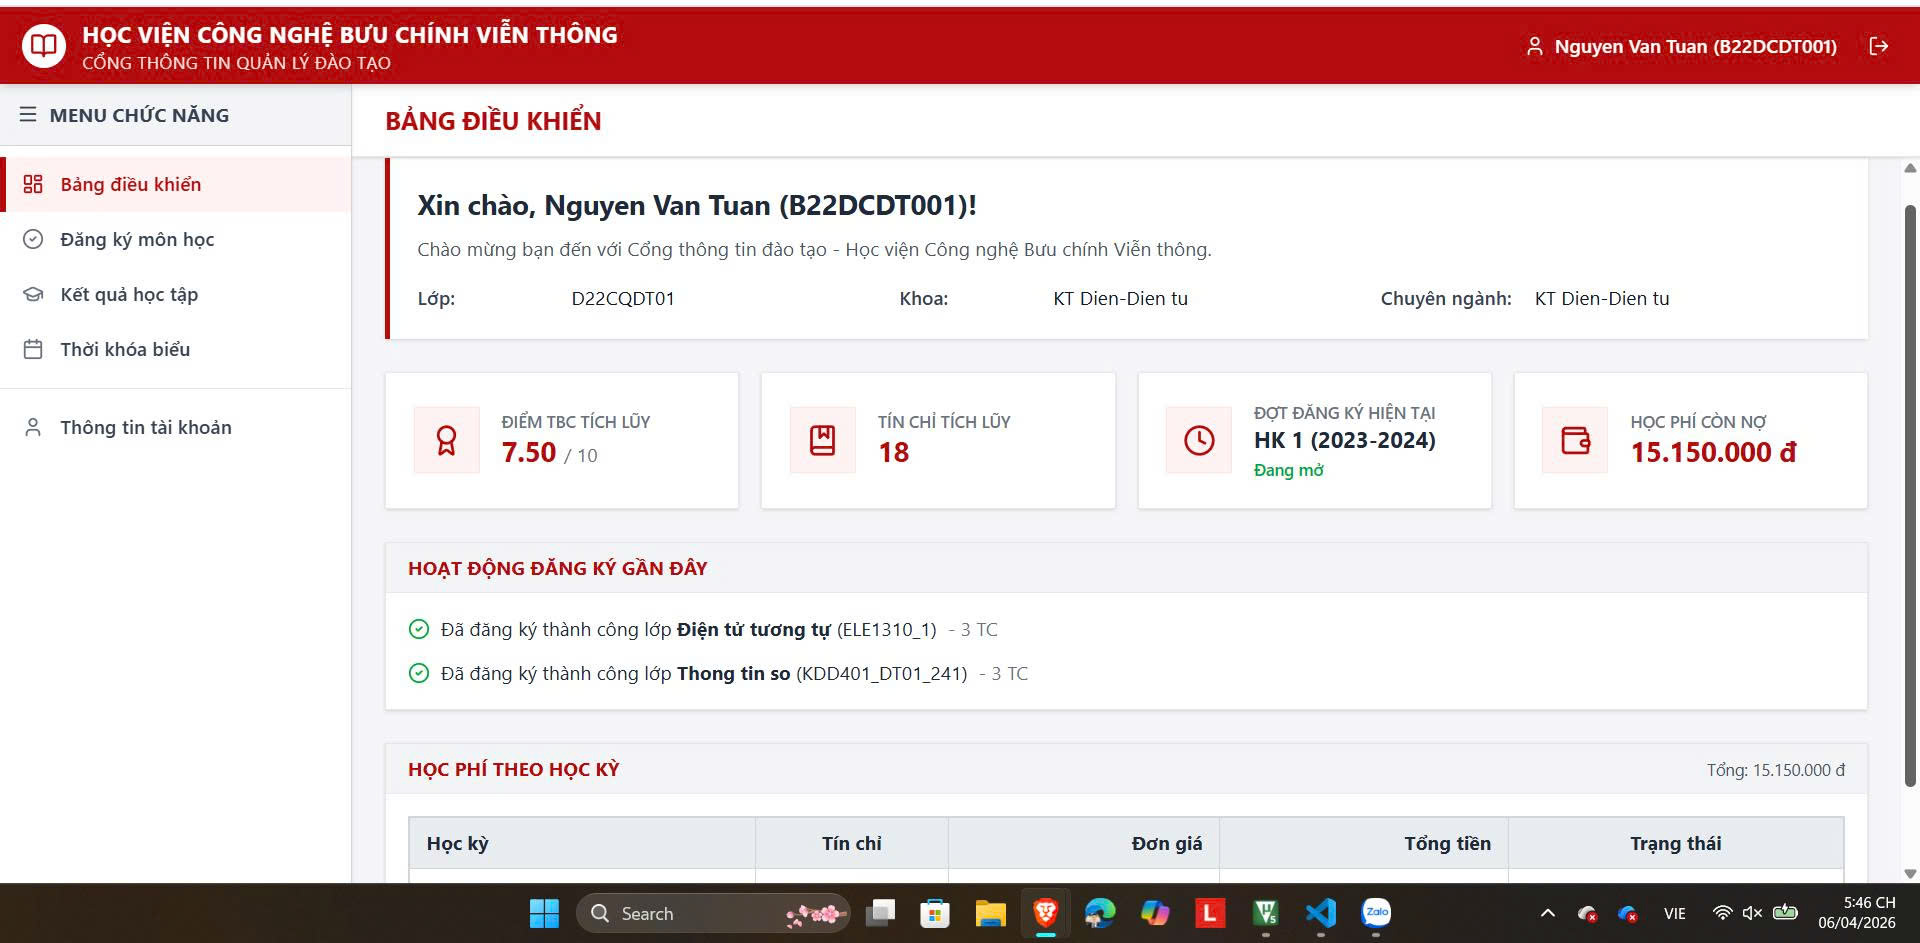
\includegraphics[width=0.95\textwidth]{image/sv_1.png}
    \caption{Giao diện sinh viên sau khi đăng nhập}
    \label{fig:ch2-sv-login}
  \end{figure}

  \item \textbf{Xem danh sách lớp học phần mở:} Hiển thị môn học, giảng viên, lịch học, sĩ số hiện tại và số chỗ còn trống.
  \begin{figure}[H]
    \centering
    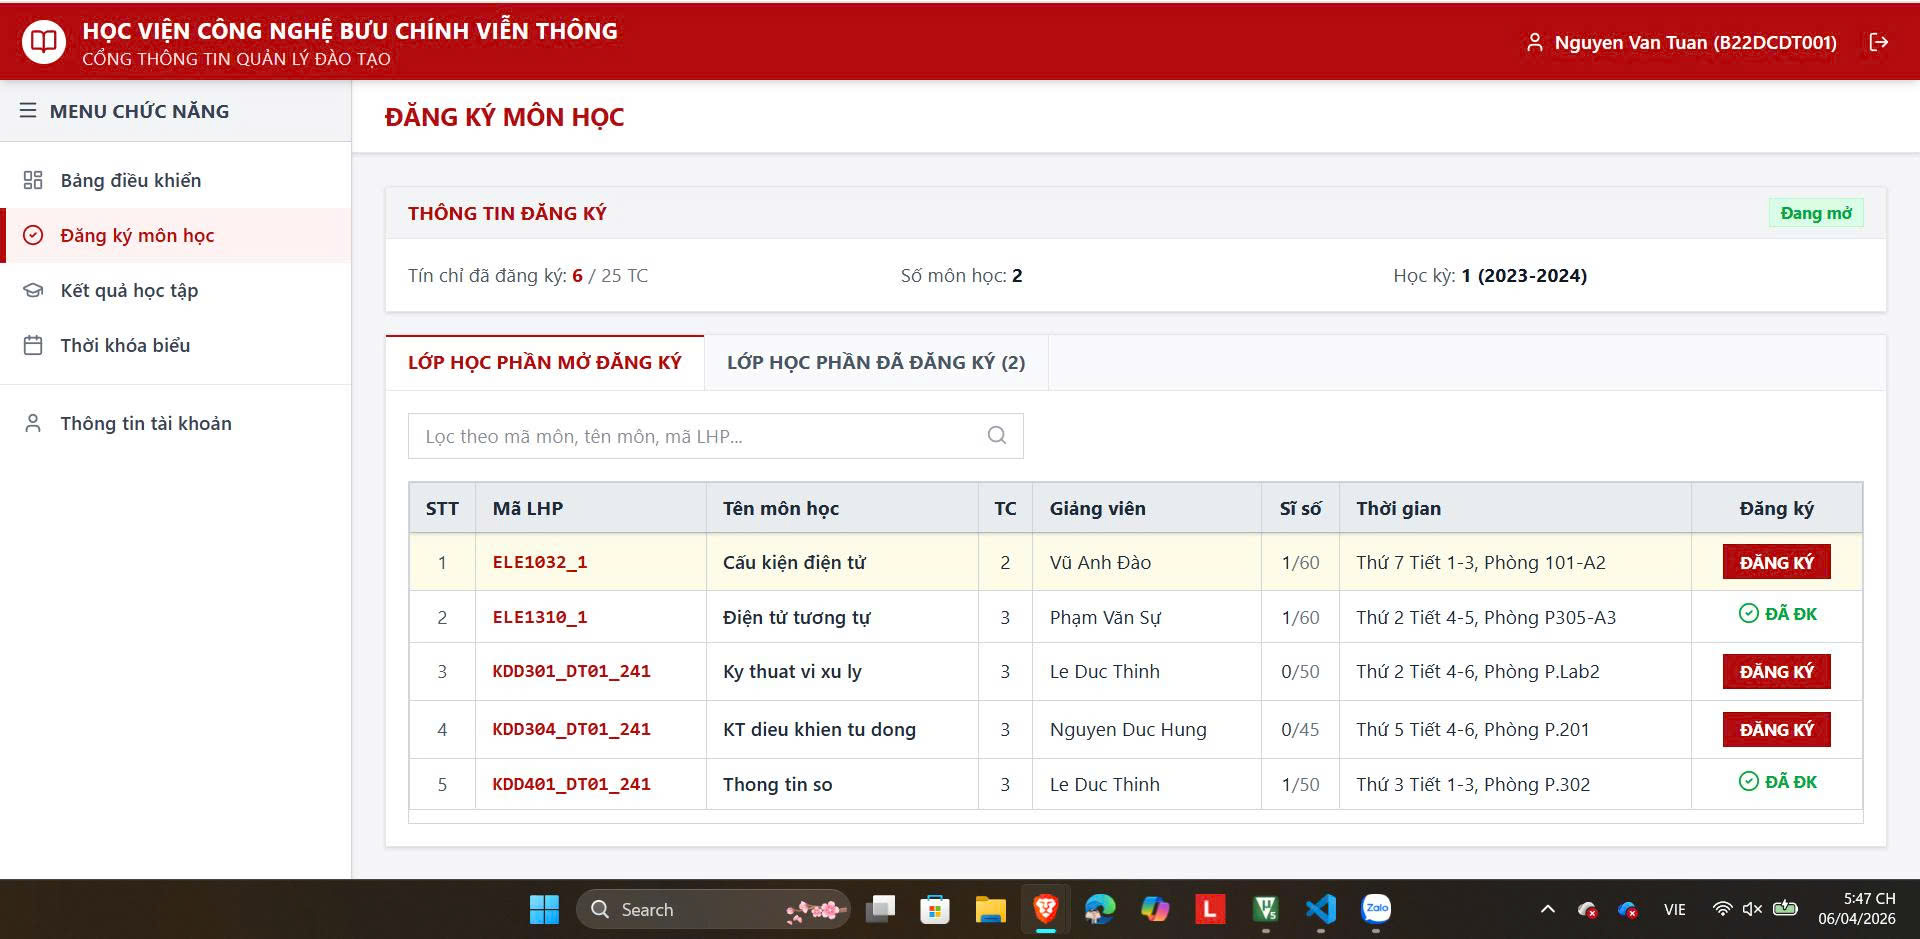
\includegraphics[width=0.95\textwidth]{image/sv2.png}
    \caption{Giao diện đăng ký học phần của sinh viên}
    \label{fig:ch2-sv-register}
  \end{figure}

  \item \textbf{Đăng ký tín chỉ:} Kiểm tra đầy đủ các điều kiện nghiệp vụ (đợt mở, không trùng lớp, đủ tiên quyết, không trùng lịch, không vượt giới hạn tín chỉ) trước khi ghi vào \texttt{DANGKY}.
  \item \textbf{Hủy đăng ký:} Chỉ thực hiện khi đợt đăng ký còn mở; học phí học kỳ được cập nhật tương ứng.
  \begin{figure}[H]
    \centering
    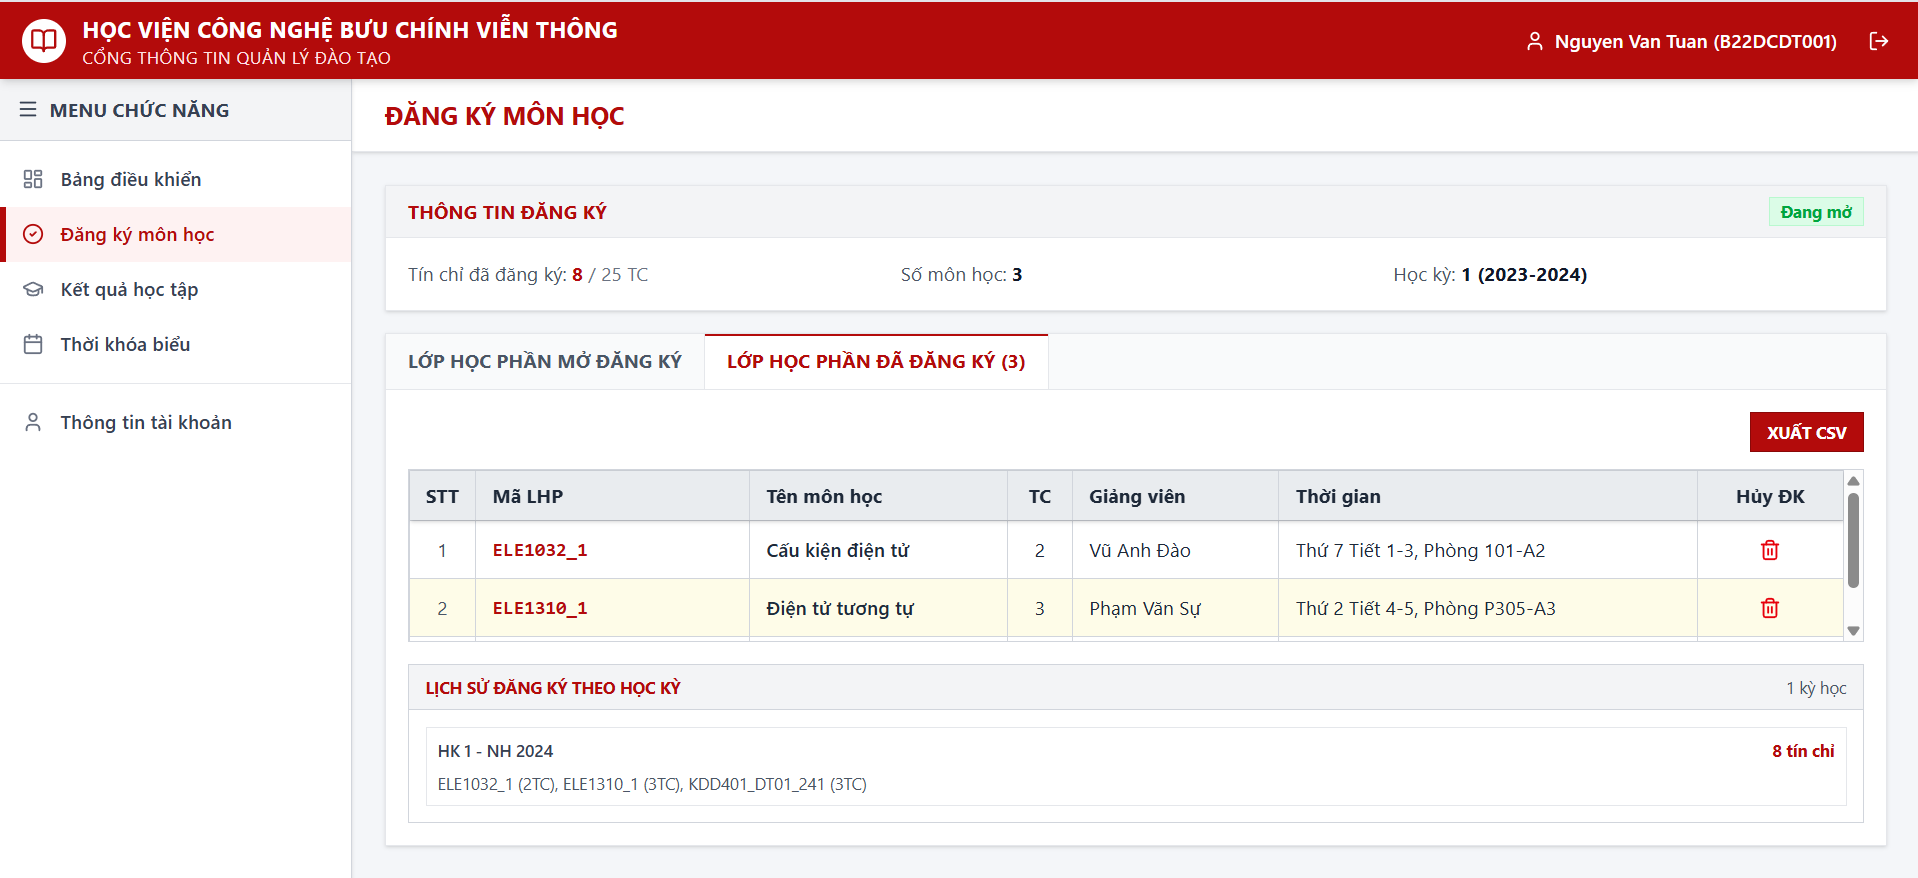
\includegraphics[width=0.95\textwidth]{image/sv3.png}
    \caption{Danh sách học phần sinh viên đã đăng ký}
    \label{fig:ch2-sv-registered}
  \end{figure}

  \item \textbf{Tra cứu kết quả học tập:} Đọc dữ liệu từ \texttt{KETQUA\_HOCTAP}, hỗ trợ hiển thị nhiều lần học một môn.
  \begin{figure}[H]
    \centering
    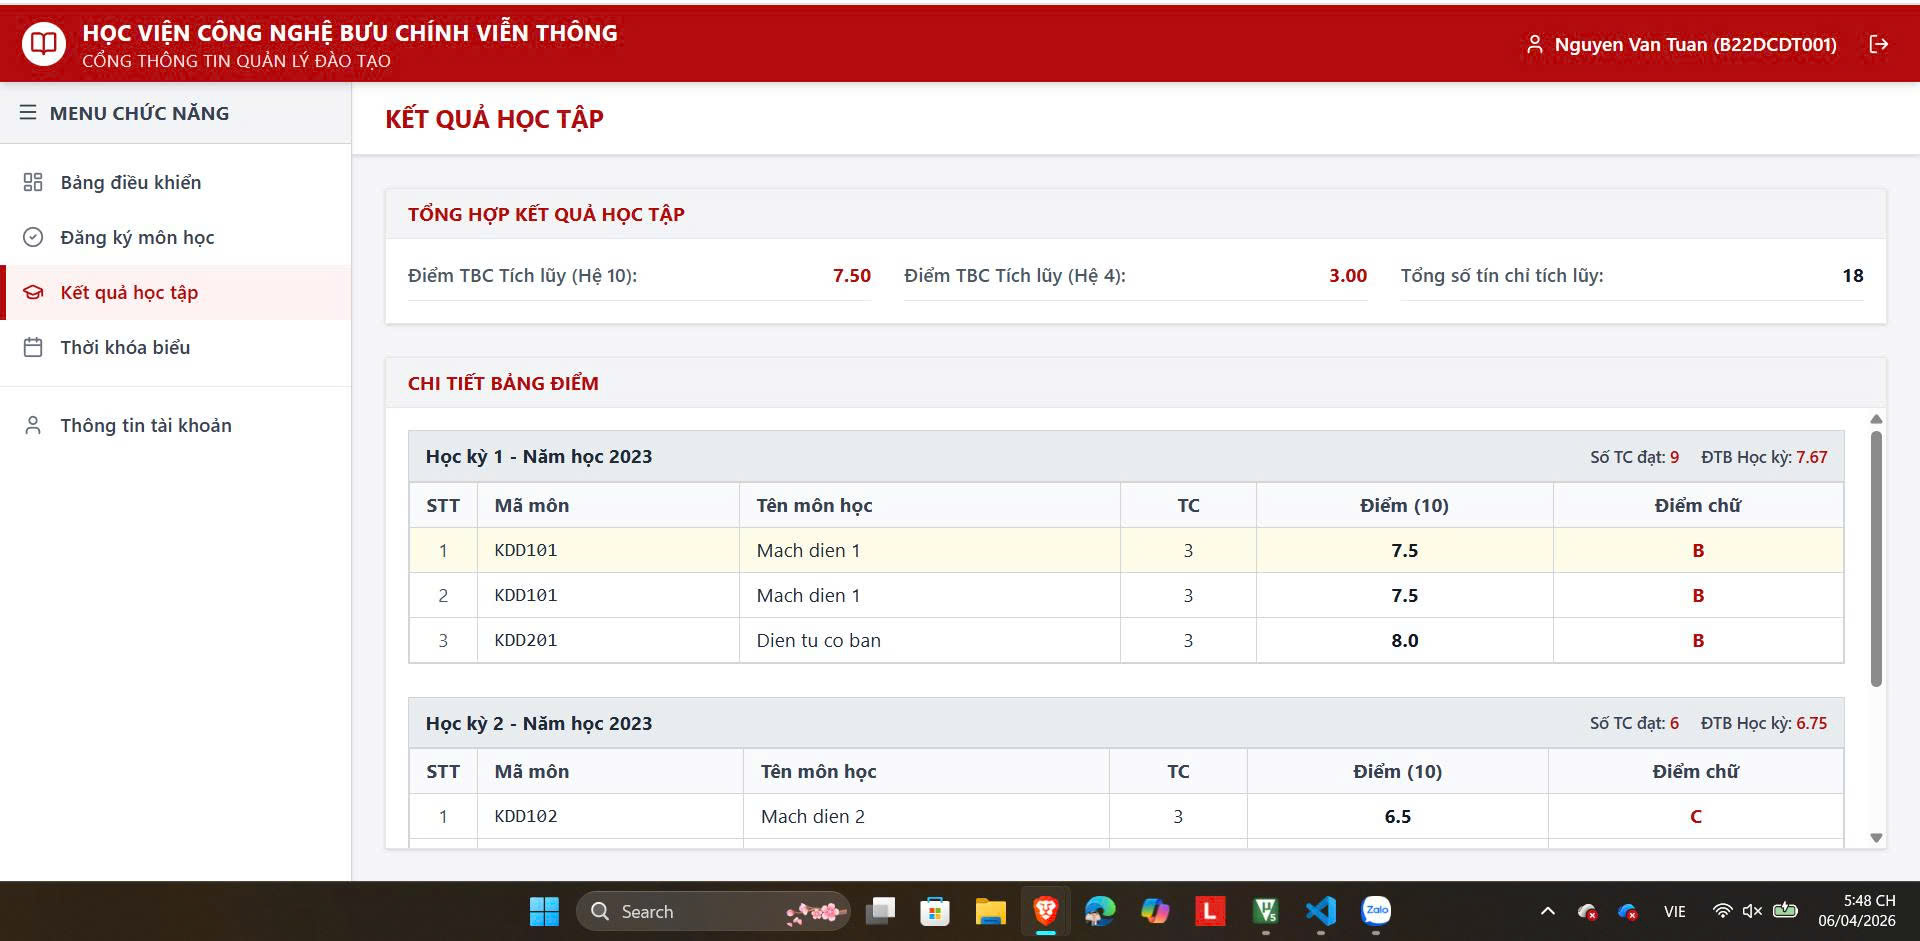
\includegraphics[width=0.95\textwidth]{image/sv4.png}
    \caption{Giao diện kết quả học tập của sinh viên}
    \label{fig:ch2-sv-result}
  \end{figure}

  \item \textbf{Theo dõi học phí:} Xem số tín chỉ, đơn giá, tổng tiền và trạng thái thanh toán theo từng học kỳ.
\end{itemize}

\subsubsection{Nhóm chức năng cho Giảng viên}
\begin{itemize}[leftmargin=1.5cm]
  \item \textbf{Xem lớp phụ trách:} Theo dõi danh sách lớp học phần được phân công.
  \begin{figure}[H]
    \centering
    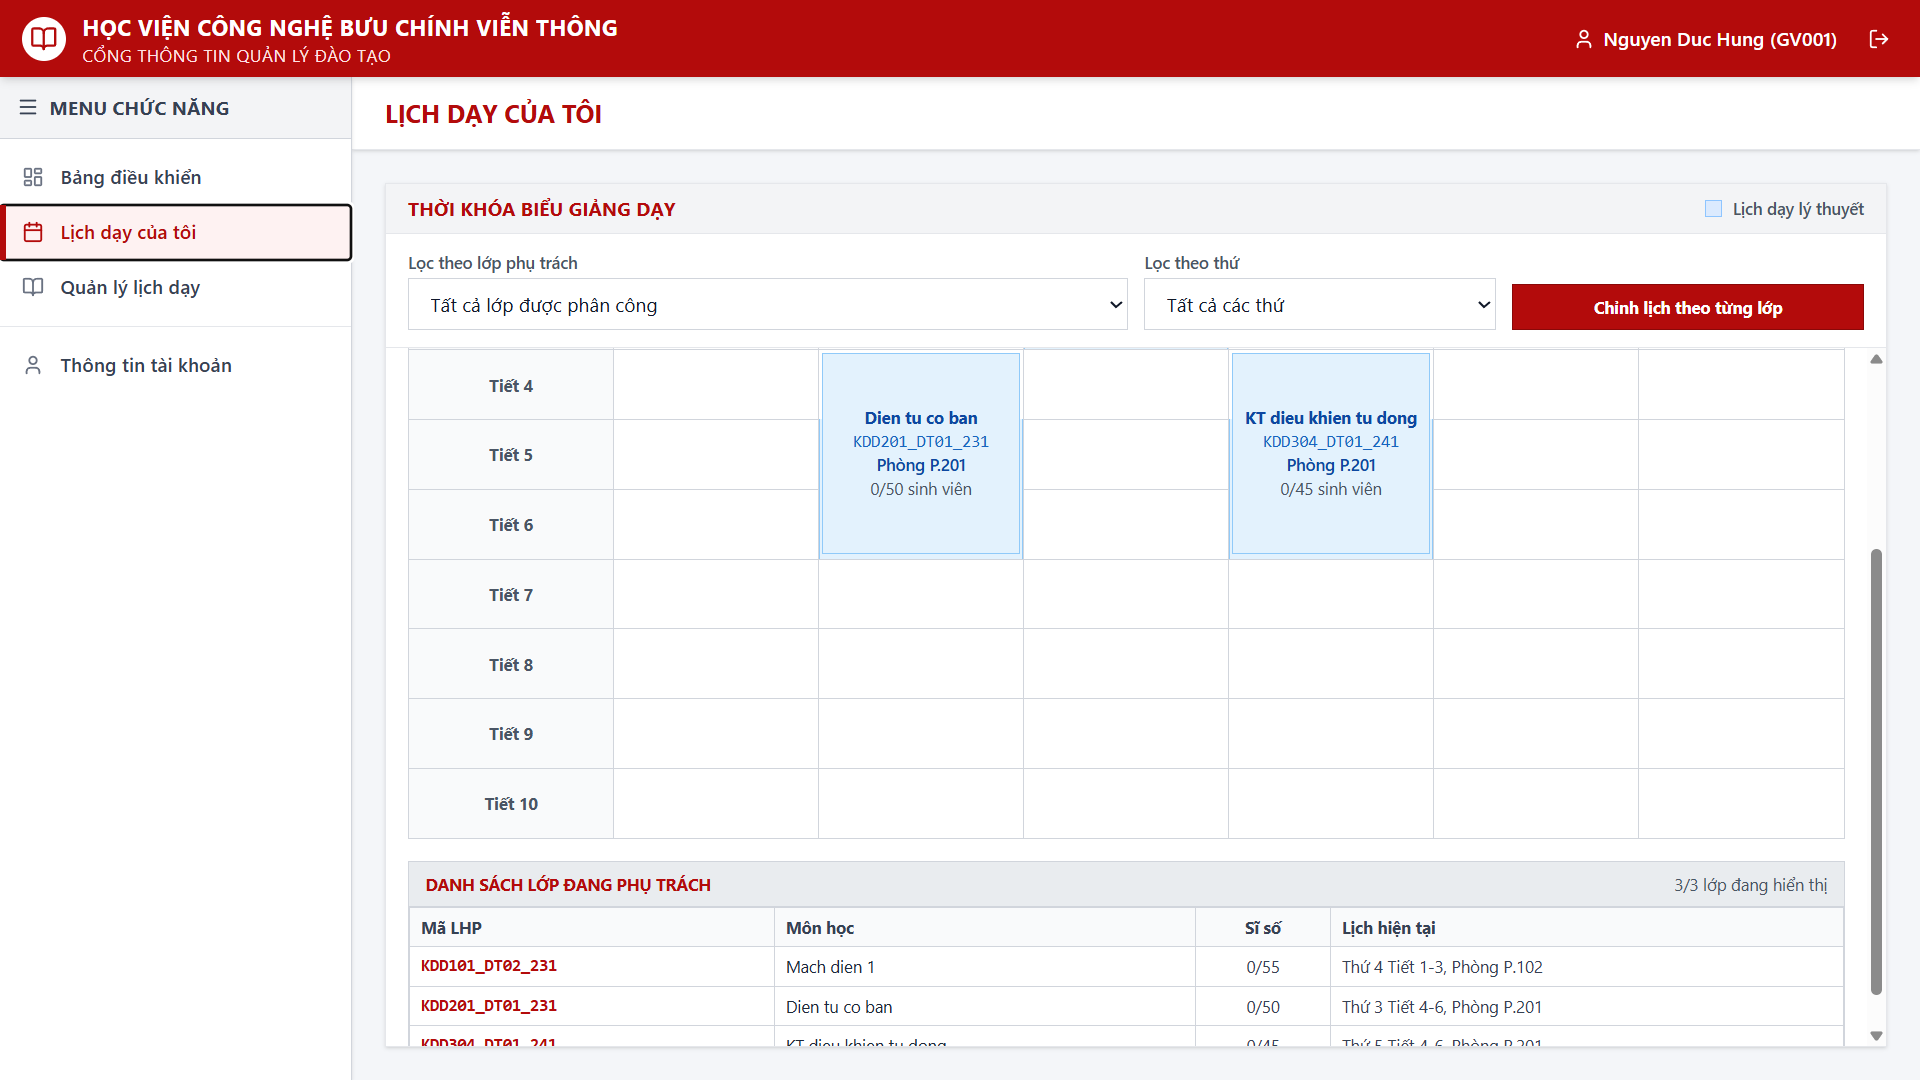
\includegraphics[width=0.95\textwidth]{image/gv2.png}
    \caption{Giao diện lớp học phần và lịch dạy của giảng viên}
    \label{fig:ch2-gv-class}
  \end{figure}

  \item \textbf{Quản lý lịch dạy:} Thêm/sửa/xóa lịch học trên bảng \texttt{LICHHOC}.
  \begin{figure}[H]
    \centering
    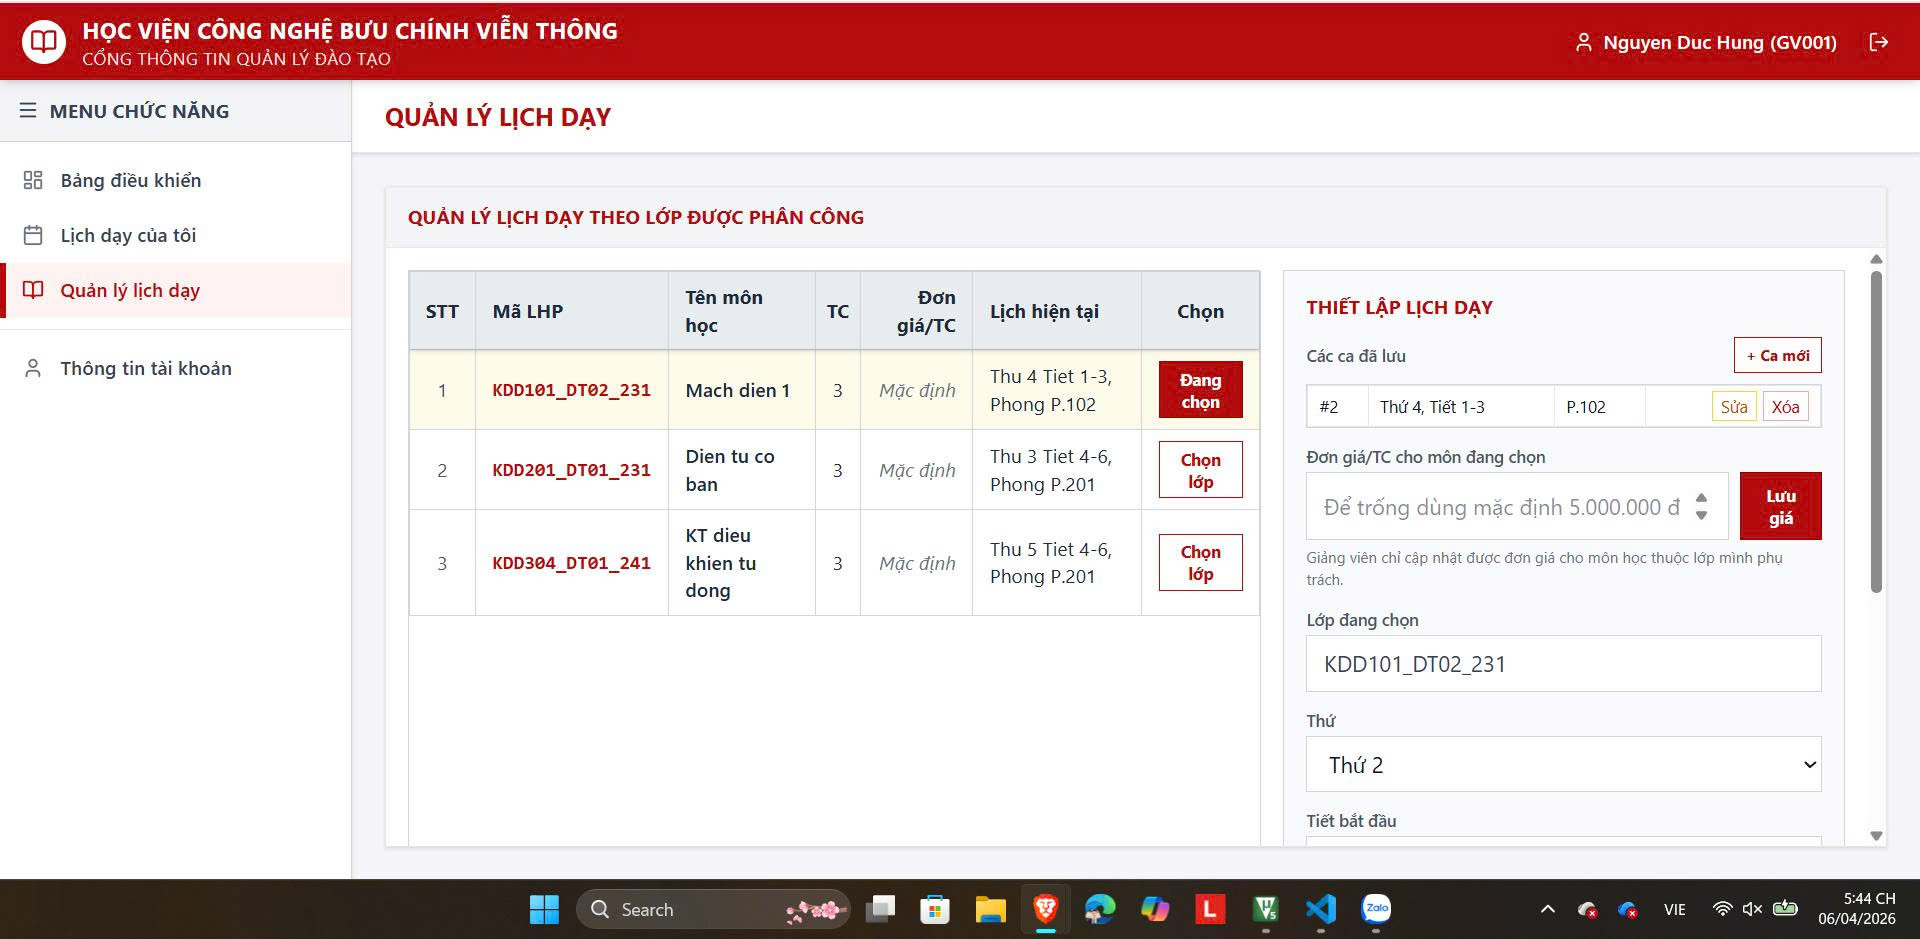
\includegraphics[width=0.95\textwidth]{image/gv1.png}
    \caption{Giao diện cập nhật lịch dạy của giảng viên}
    \label{fig:ch2-gv-schedule}
  \end{figure}

  \item \textbf{Theo dõi tình trạng đăng ký:} Quan sát số lượng sinh viên đăng ký từng lớp để chủ động tổ chức giảng dạy.
\end{itemize}

\subsubsection{Nhóm chức năng cho Quản trị viên}
\begin{itemize}[leftmargin=1.5cm]
  \item \textbf{Quản lý người dùng:} Thêm/sửa/xóa/khôi phục tài khoản sinh viên và giảng viên.
  \begin{figure}[H]
    \centering
    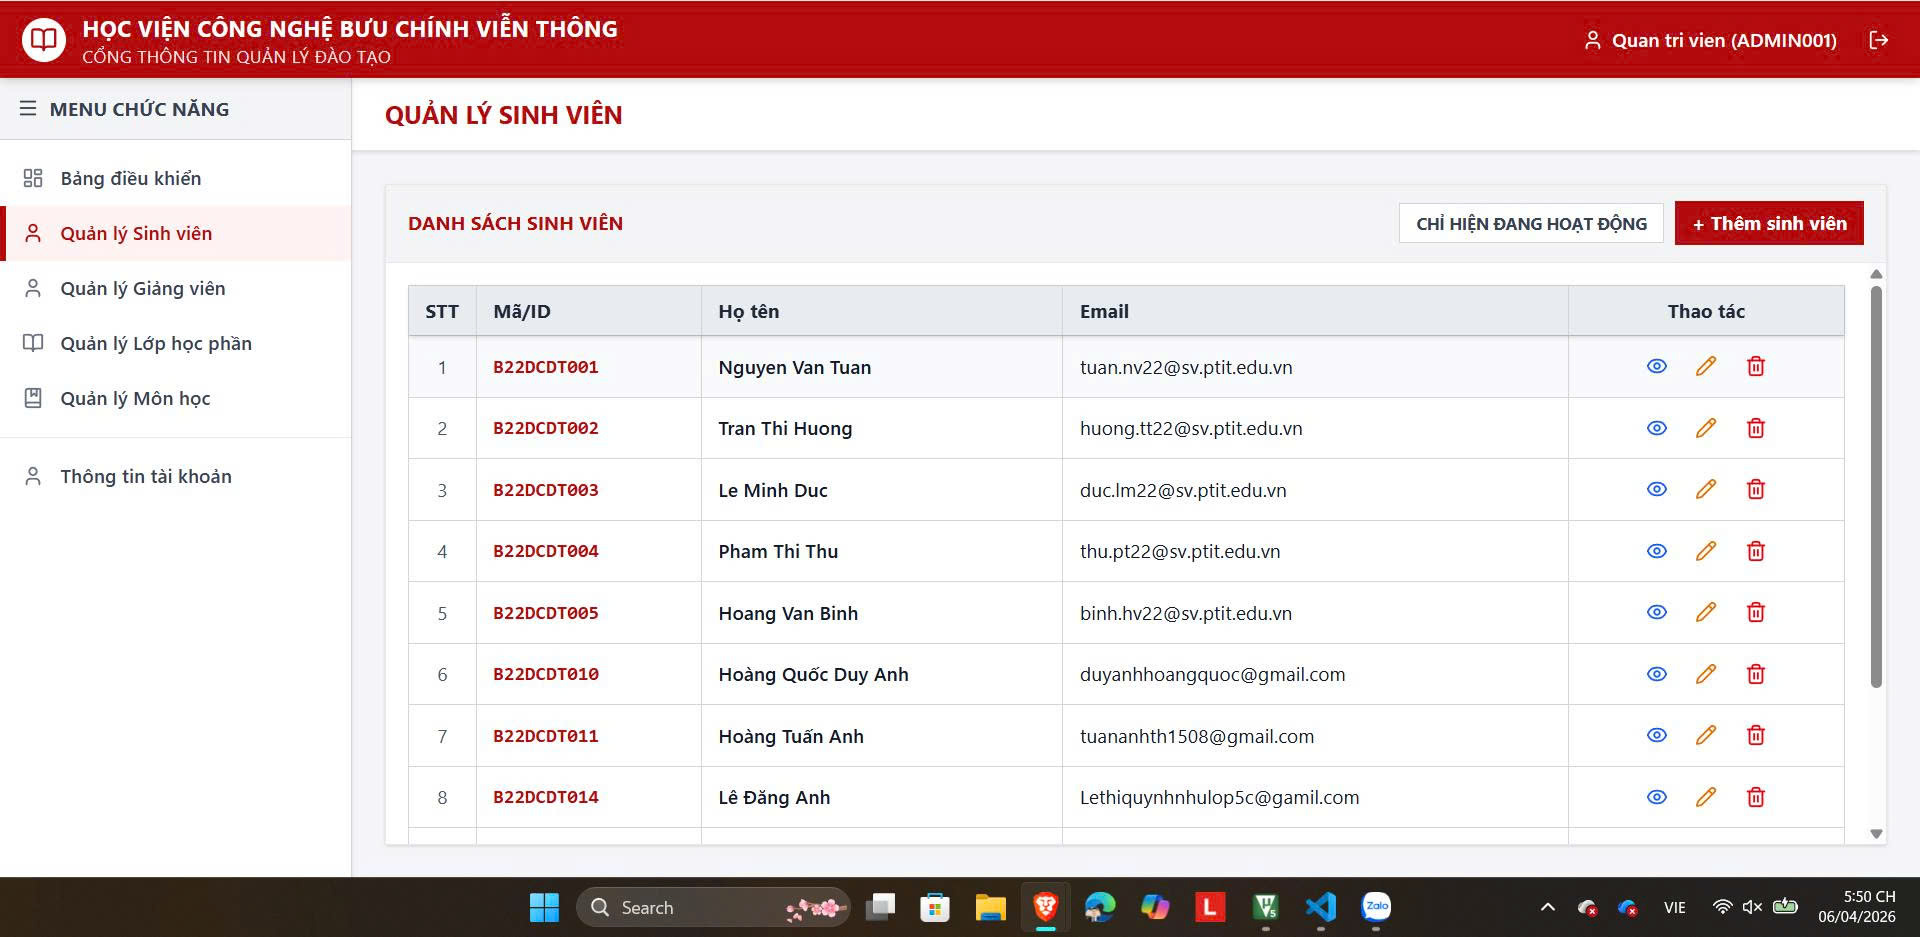
\includegraphics[width=0.95\textwidth]{image/ad1.png}
    \caption{Giao diện quản lý tài khoản sinh viên}
    \label{fig:ch2-ad-student}
  \end{figure}

  \begin{figure}[H]
    \centering
    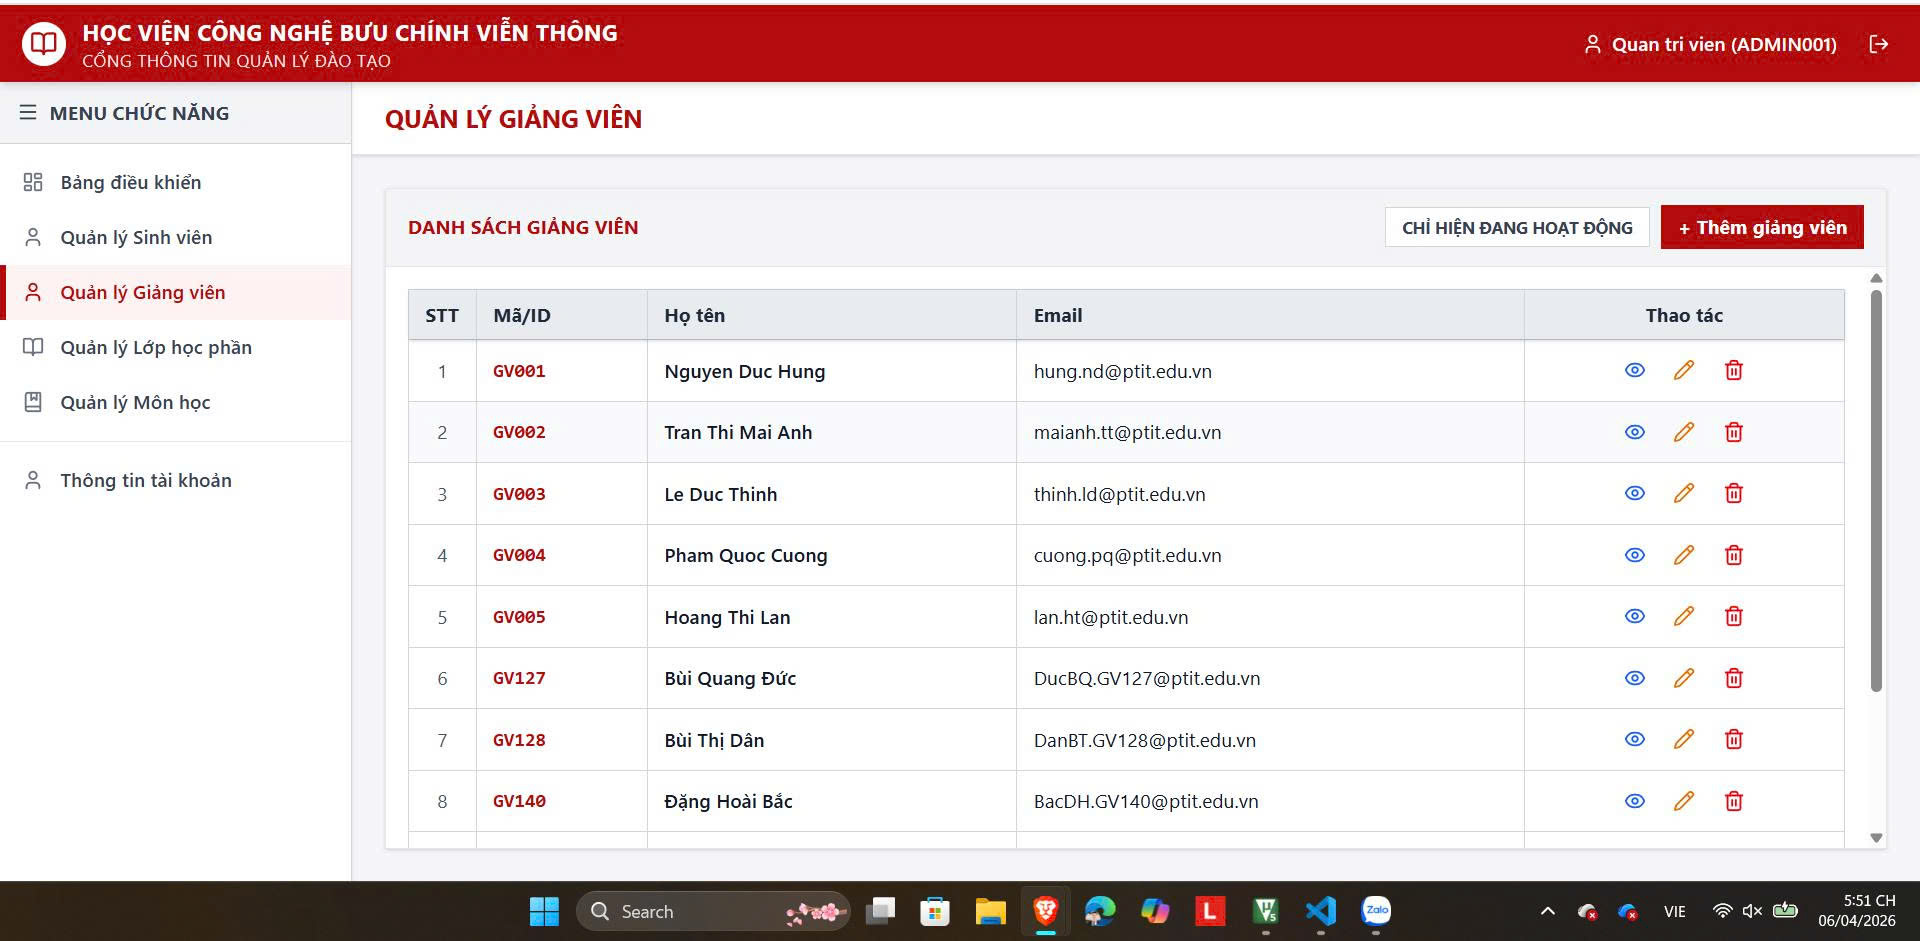
\includegraphics[width=0.95\textwidth]{image/ad2.png}
    \caption{Giao diện quản lý tài khoản giảng viên}
    \label{fig:ch2-ad-teacher}
  \end{figure}

  \item \textbf{Quản lý môn học và lớp học phần:} Tạo mới, cập nhật, kiểm tra phụ thuộc dữ liệu trước khi xóa.
  \begin{figure}[H]
    \centering
    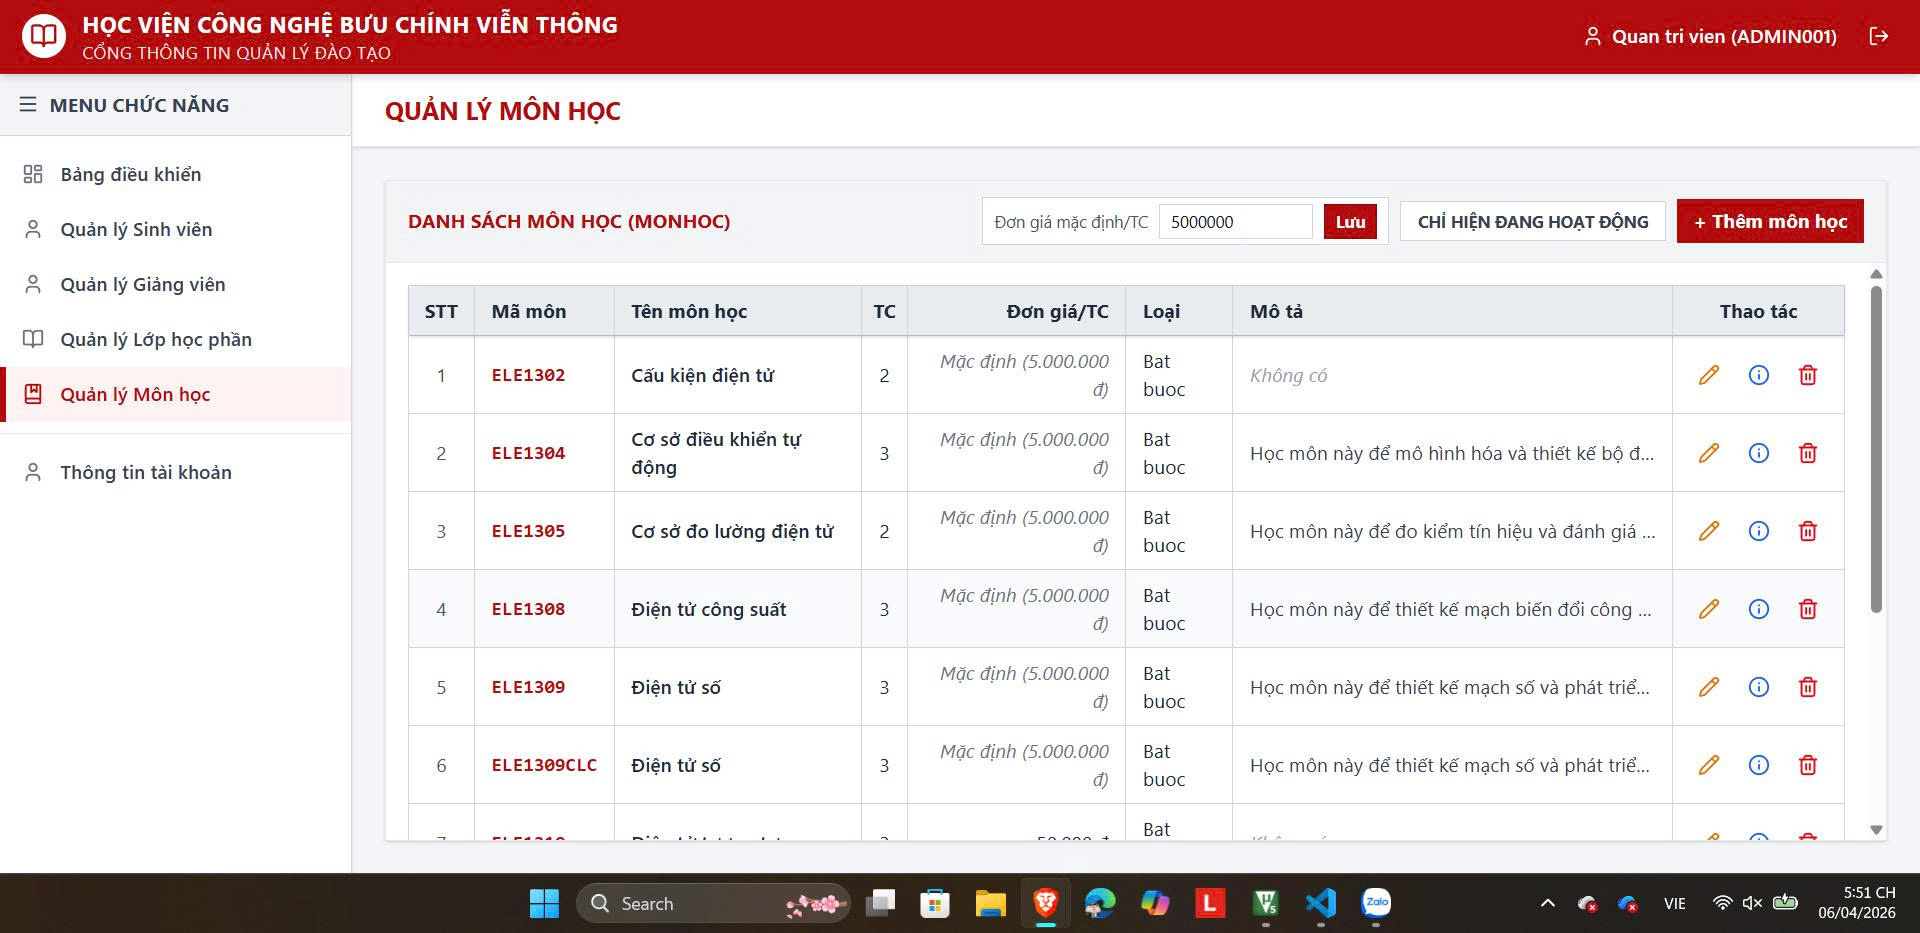
\includegraphics[width=0.95\textwidth]{image/ad3.png}
    \caption{Giao diện quản lý danh mục môn học}
    \label{fig:ch2-ad-course}
  \end{figure}

  \begin{figure}[H]
    \centering
    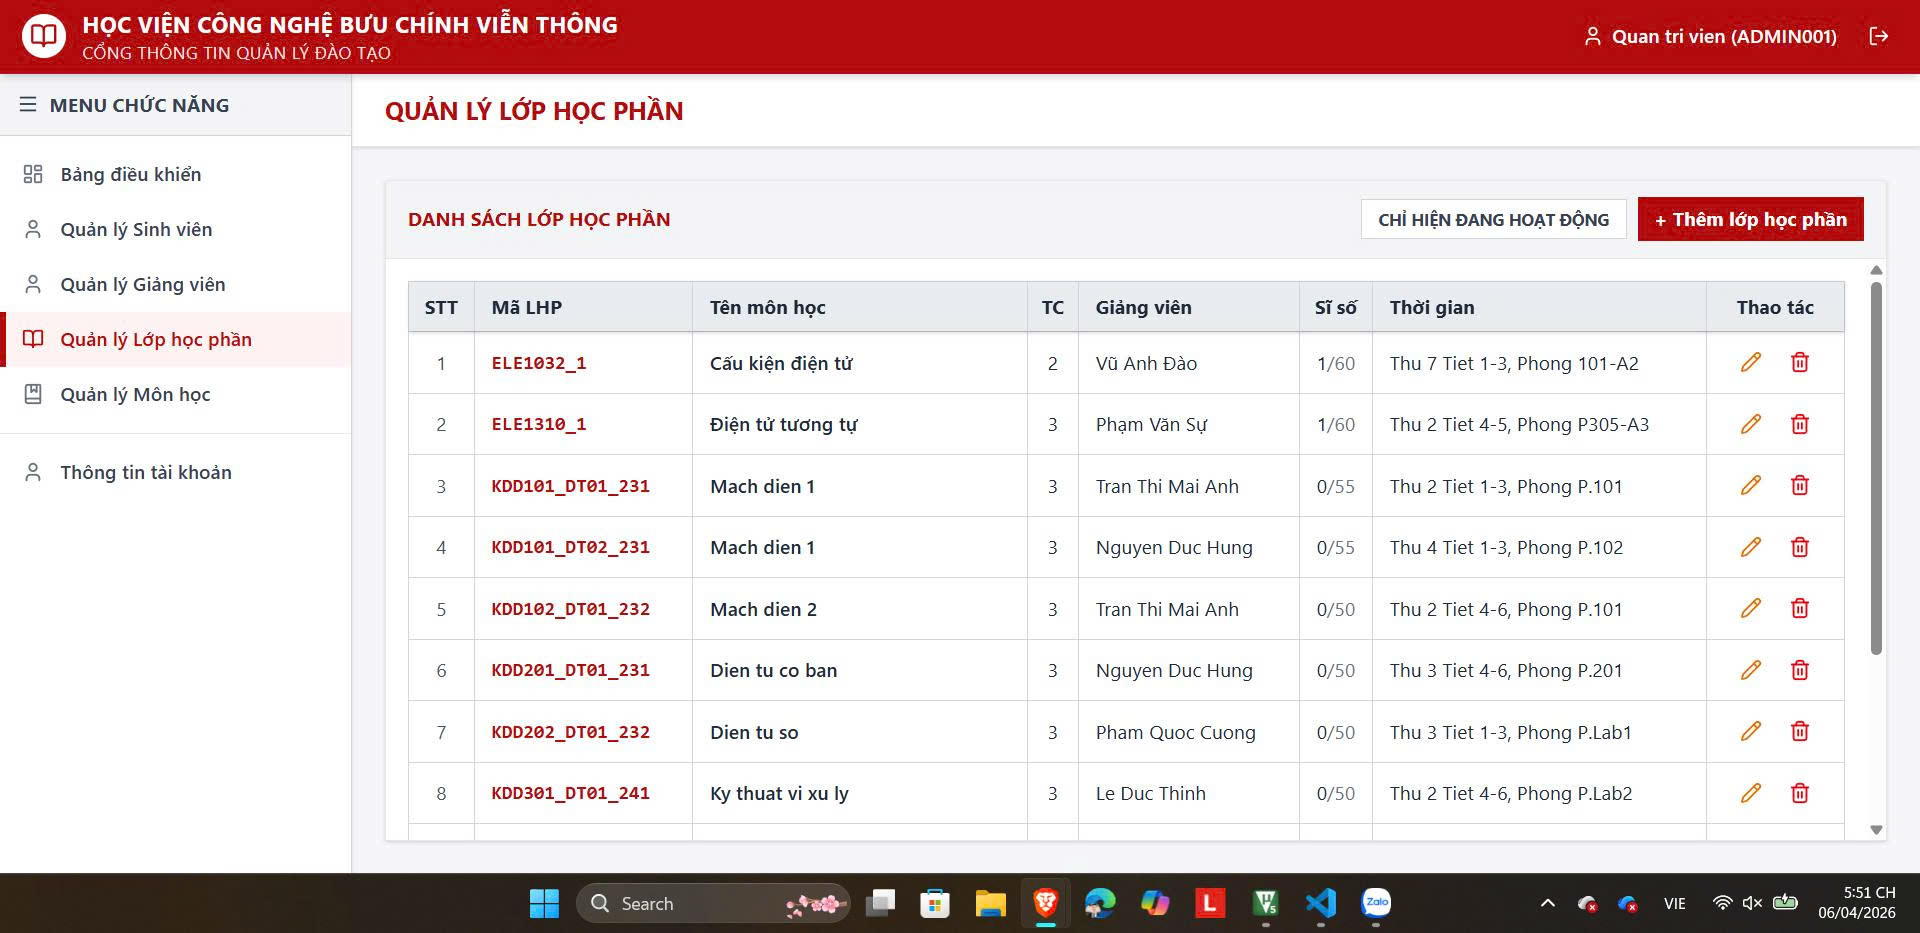
\includegraphics[width=0.95\textwidth]{image/ad4.png}
    \caption{Giao diện quản lý lớp học phần}
    \label{fig:ch2-ad-class}
  \end{figure}

  \item \textbf{Import dữ liệu CSV:} Nạp dữ liệu ban đầu từ các tệp mẫu.
  \begin{figure}[H]
    \centering
    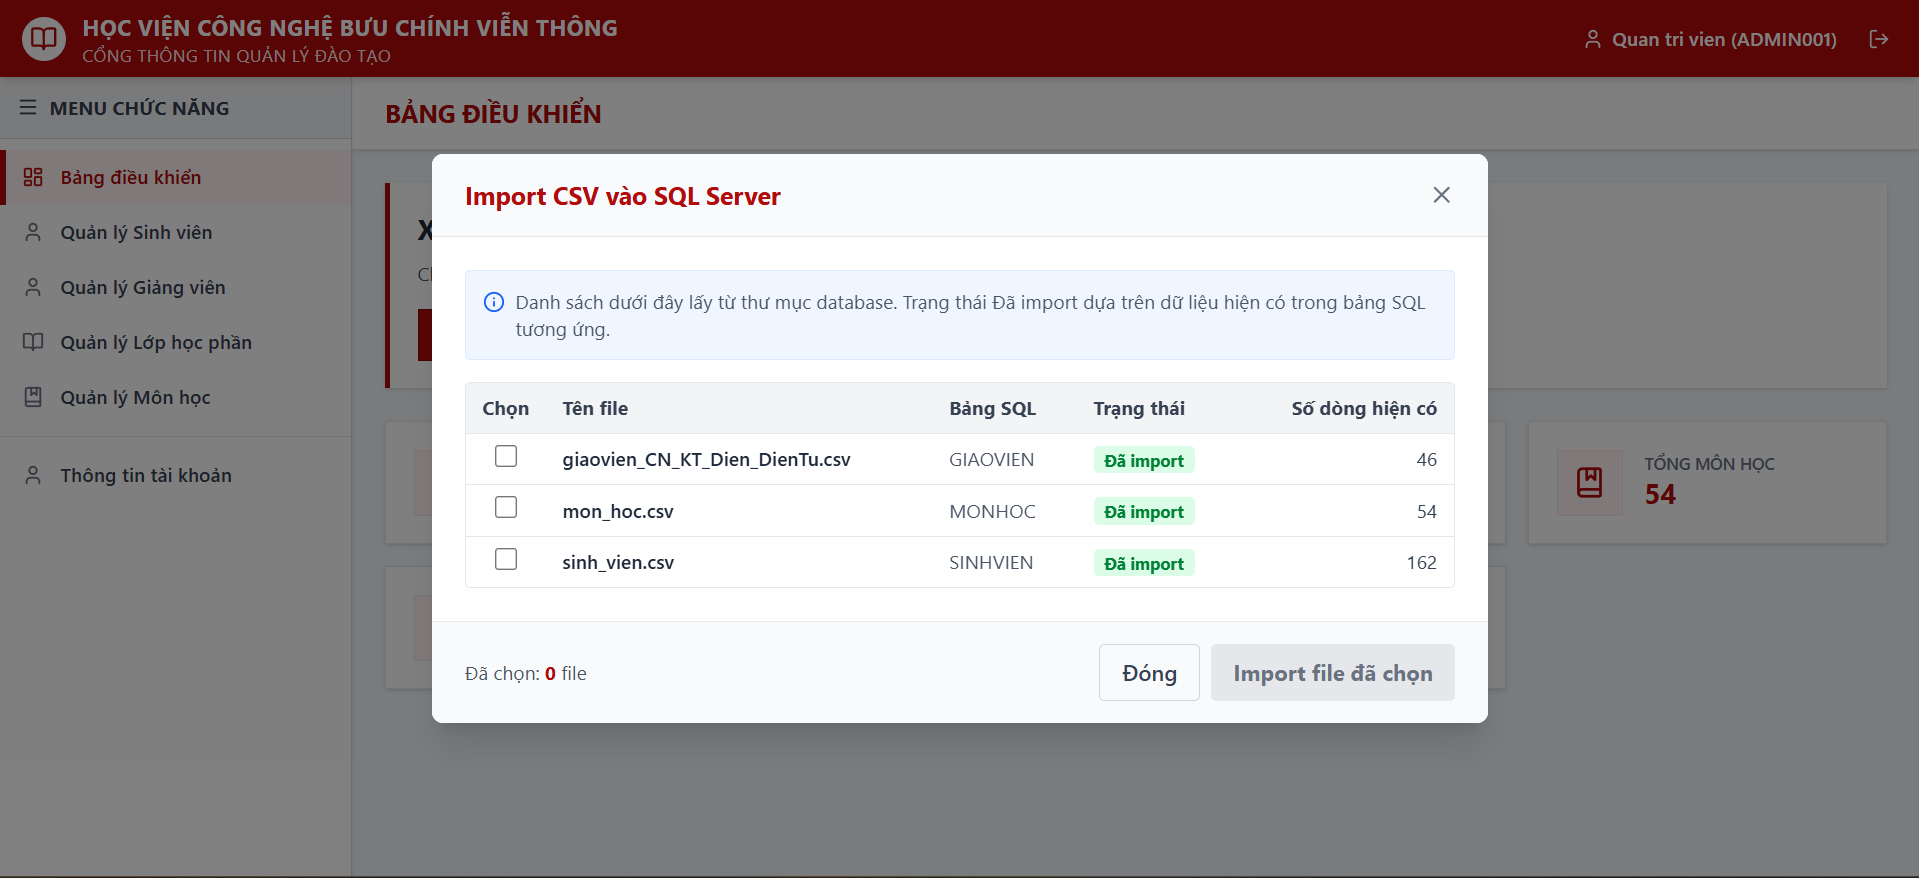
\includegraphics[width=0.95\textwidth]{image/ad5.png}
    \caption{Giao diện import dữ liệu CSV}
    \label{fig:ch2-ad-import}
  \end{figure}

  \item \textbf{Theo dõi báo cáo vận hành:} Tổng số lớp mở, số lượt đăng ký, tỷ lệ lấp đầy và tổng học phí phát sinh.
  \begin{figure}[H]
    \centering
    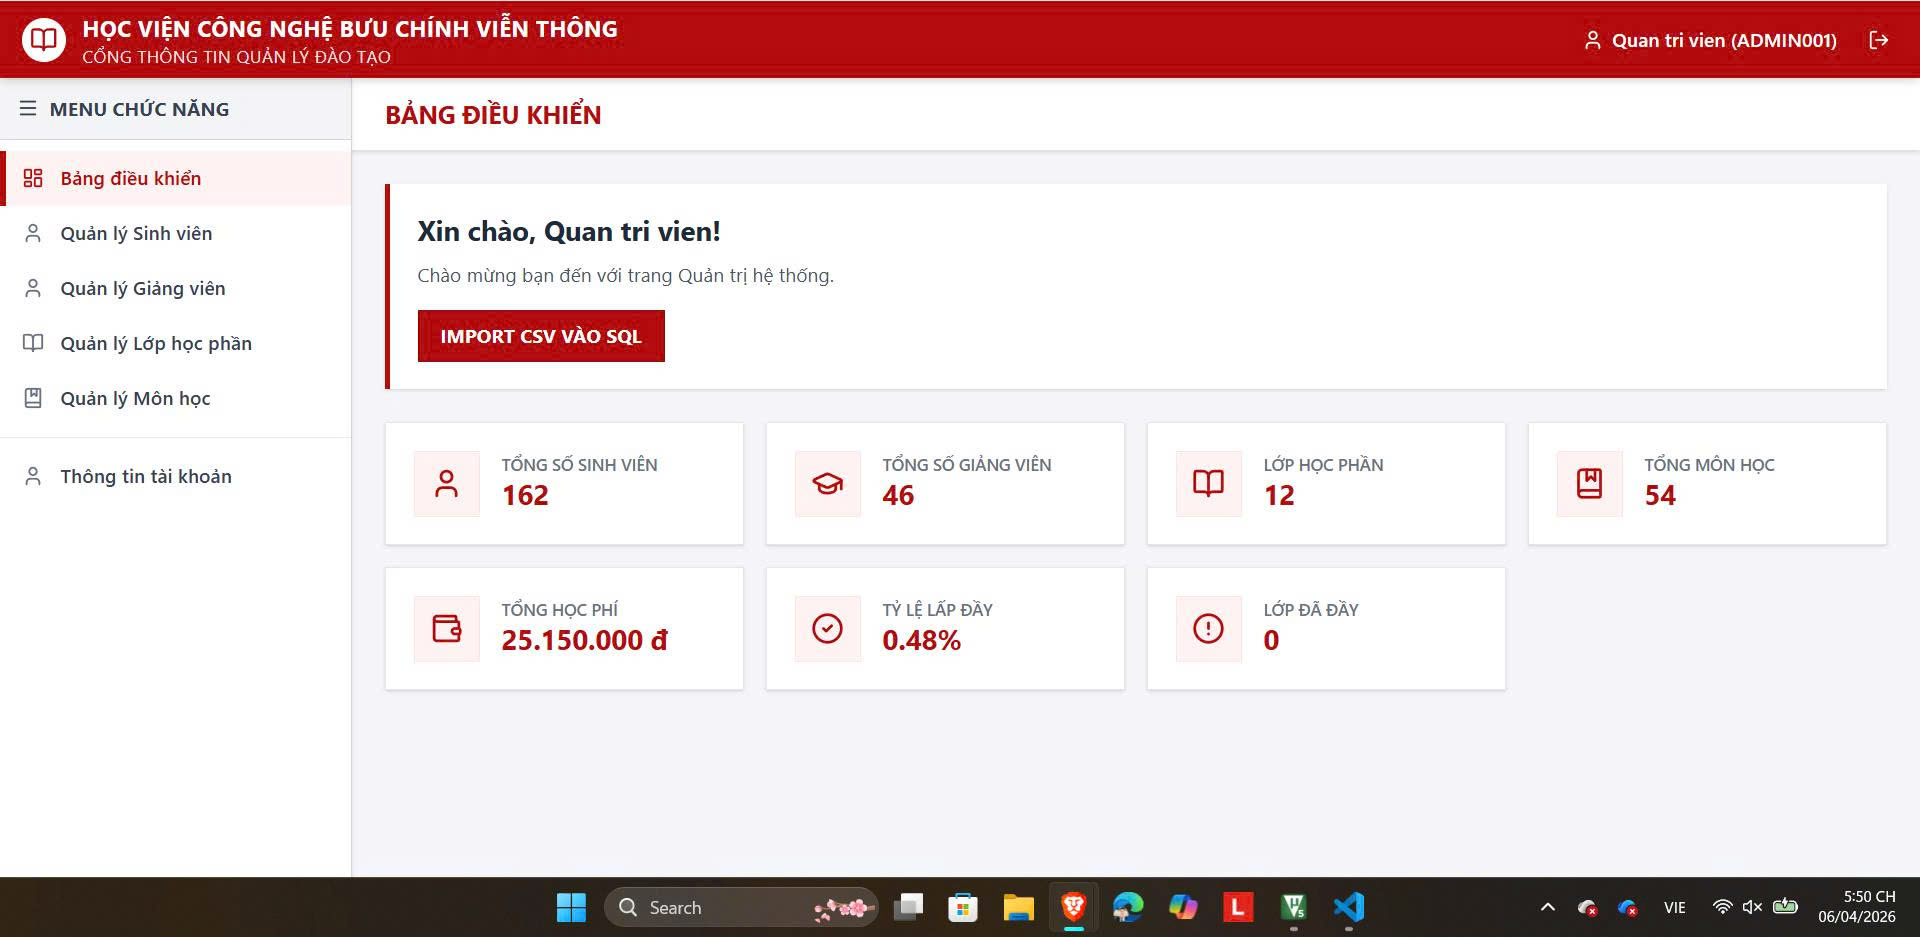
\includegraphics[width=0.95\textwidth]{image/ad6.png}
    \caption{Giao diện báo cáo vận hành hệ thống}
    \label{fig:ch2-ad-report}
  \end{figure}
\end{itemize}

\subsection{Đảm bảo toàn vẹn dữ liệu khi vận hành}

\noindent Tính đúng đắn dữ liệu được bảo đảm theo mô hình kiểm tra nhiều lớp:
\begin{itemize}[leftmargin=1.5cm]
  \item \textbf{Lớp ứng dụng:} Kiểm tra đầu vào và phân quyền theo vai trò.
  \item \textbf{Lớp thủ tục/trigger:} Chặn các trường hợp vi phạm nghiệp vụ trong đăng ký, hủy đăng ký, cập nhật điểm.
  \item \textbf{Lớp ràng buộc CSDL:} Duy trì toàn vẹn khóa chính/khóa ngoại, CHECK, UNIQUE và computed column.
\end{itemize}

\subsection{Đánh giá kết quả triển khai}

\noindent Kết quả thử nghiệm cho thấy các chức năng lõi trên ứng dụng hoạt động ổn định và đồng bộ với CSDL. Đây là nền tảng để mở rộng các module tiếp theo như lịch thi, thanh toán học phí trực tuyến và dashboard phân tích nâng cao.

% ============================================================
%  KẾT LUẬN
% ============================================================
\newpage
\section*{KẾT LUẬN}
\addcontentsline{toc}{section}{Kết luận}

\noindent Qua quá trình nghiên cứu và thực hiện bài tập lớn, nhóm đã hoàn thành việc thiết kế và xây dựng hệ thống cơ sở dữ liệu quản lý đăng ký tín chỉ với 7 module chức năng. Các kết quả đạt được bao gồm:

\begin{itemize}[leftmargin=1.5cm]
  \item Phân tích và thiết kế \textbf{14 bảng} phản ánh đầy đủ các thực thể và nghiệp vụ của hệ thống, bao gồm CHUONGTRINH\_DAOTAO, LICHHOC, KETQUA\_HOCTAP, HOCPHI và QUANTRI.
  \item Thiết kế tách bạch giữa \textbf{DANGKY} (hành động đăng ký) và \textbf{KETQUA\_HOCTAP} (điểm số với LanHoc), hỗ trợ học lại nhiều lần và đảm bảo toàn vẹn dữ liệu.
  \item Chuẩn hóa lịch học sang bảng \textbf{LICHHOC} với dữ liệu số (Thu, TietBatDau, SoTiet), cho phép kiểm tra trùng lịch chính xác bằng điều kiện overlap $[A,A+s_A) \cap [B,B+s_B) \neq \emptyset$.
  \item Chứng minh tất cả \textbf{14 bảng đạt 3NF}; riêng YEUCAU\_TIENQUYET và CTDT\_MONHOC còn đạt BCNF.
  \item Triển khai \textbf{6 Stored Procedure}, \textbf{4 Trigger} (kiểm tra sỹ số, trùng lịch, cập nhật kết quả, tính học phí tự động), \textbf{5 View} phân tích và hệ thống \textbf{phân quyền 3 ROLE}.
  \item Tối ưu hiệu năng với \textbf{8 chỉ mục} non-clustered, đặc biệt chỉ mục kép trên LICHHOC(MaLopHP, Thu, TietBatDau) để tăng tốc kiểm tra trùng lịch.
\end{itemize}

\vspace{0.4cm}
\noindent \textbf{Hạn chế và hướng phát triển:} Hệ thống hiện tại chưa bao gồm quản lý lịch thi, học bổng và miễn giảm học phí theo từng sinh viên cụ thể. Về bảo mật, cơ chế xác thực hiện tại lưu hash SHA-256 đơn giản -- trong môi trường production nên nâng cấp lên bcrypt hoặc Argon2 (có salt ngẫu nhiên) để chống tấn công rainbow table. Trong tương lai, nhóm đề xuất bổ sung bảng LICHITHI và tích hợp Row-level Security (RLS Policy) để sinh viên chỉ xem được dữ liệu của chính mình.

% ============================================================
%  TÀI LIỆU THAM KHẢO
% ============================================================
\newpage
\begin{thebibliography}{9}
\addcontentsline{toc}{section}{Tài liệu tham khảo}

\bibitem{elmasri}
  Ramez Elmasri, Shamkant Navathe.
  \textit{Fundamentals of Database Systems}, 7th Edition.
  Pearson, 2015.

\bibitem{silberschatz}
  Abraham Silberschatz, Henry F. Korth, S. Sudarshan.
  \textit{Database System Concepts}, 7th Edition.
  McGraw-Hill, 2019.

\bibitem{date}
  C. J. Date.
  \textit{An Introduction to Database Systems}, 8th Edition.
  Addison-Wesley, 2003.

\bibitem{mssql}
  Microsoft.
  \textit{Transact-SQL Reference (Database Engine)}, 2024.
  \url{https://docs.microsoft.com/en-us/sql/t-sql/}

\bibitem{bgddt}
  Bộ Giáo dục và Đào tạo.
  \textit{Quy chế đào tạo đại học theo hệ thống tín chỉ}.
  Thông tư 08/2021/TT-BGDĐT, 2021.

\end{thebibliography}

\end{document}